In this chapter we recall the dynamics of the system whose weights have already been shaped by a previous learning experience. We will describe the system as a network of identical oscillators coupled via their nonlinear output. Then, via bifurcation analysis, we will characterise the qualitative behaviour of a simple 4-dimensional oscillator, with respect to the parameters that characterise the dynamics of the system. In the final section we study under which condition on the graph connectivity synchronization occurs.

\section{Free Recall Dynamics}
\paragraph{Assumptions}
Before going further we present the crucial assumptions that will be kept fixed for all the analysis:
 \begin{itemize}
     \item \textbf{A1} The undirected graph describing network's interaction is fixed, shaped by a previous learning experience.
     \item \textbf{A2} Once the coupling weights have been learned, the input signal to the units is removed and the network evolves without any external input.
     \item \textbf{A3} The patterns stored are orthogonal, i.e. each minicolumn is active in one and only one pattern. At the weights level this means that minicolumns that are supposed to fire together are positively coupled with no more than one minicolumn for each of the other hypercolumns. 
     \item \textbf{A4} We assume the existence of a self-excitation term whose principal function is to regularise the activity of each hypercolumn. 
 \end{itemize}
 
\paragraph{Network Description}
Consider a generic system made of $h$ units (hypercolumns), each one made of $m$ minicolumns. Denote $s_i = [s_{i1}, \dots, s_{im}]$ and $a_i = [a_{i1}, \dots, a_{im}]$ the $m$-dimensional vectors that represent, respectively, the activities and the adaptation variables of the minicolumns in the hypercolumn $i$; $o_i = [o_{i1}, \dots, o_{im}]$ the corresponding outputs computed with the softmax distribution. The symmetric interactions between the minicolumns $ij, kl$ is mediated via their output $o_{ij}, o_{kl}$ with the weight \textbf{$w_{ijkl}$}.

Given the assumption \textbf{A2} we can consider the network structure as organised into $m$ levels as in figure \cref{fig:network_levels} with an associated graph $\mathcal{G}_i$ for each level. Nevertheless, for the sake of simplicity we initially assume that $\mathcal{G}_1 = \mathcal{G}_2 = \dots = \mathcal{G}_m$ such that it is sufficient a unique graph $\mathcal{G}$ to describe the network at the hypercolumns level. Therefore, we can write $w_{ijkl}=w_{ik},\ \forall j, l$ and denote $W =\left[w\right]_{ik}$ the symmetric adjacency matrix associated to the network. Given the previous considerations and taking into account \textbf{A4} we can write

\begin{equation}
    \frac{ds_{ij}}{dt} = \frac{\sum\limits_{k=1}^H w_{ik}o_{kj}-a_{ij}-s_{ij} + \alpha_{ij} o_{ij}}{\tau_m} 
    \label{eq:sij_net}
\end{equation}
\begin{equation}
    \frac{da_{ij}}{dt} = \frac{g_ao_{ij}-a_{ij}}{\tau_a} 
    \label{eq:aij_net}
\end{equation}
\begin{equation}
    o_{ij} = \frac{e^{s_{ij}}}{ \sum\limits_{k=1}^m e^{s_{ik}}}
    \label{eq:oij_net}
\end{equation}
Under the assumption that $\sum\limits_{k=1}^H w_{ik} + \alpha_{ij}=k, \forall i \in \{1, 2, ..., h\}$ \todo{to be justified properly, but atm it's fine} it is particularly convenient to rewrite \cref{eq:sij_net} in the following form:
\begin{equation}
    \frac{ds_{ij}}{dt} = \frac{\sum\limits_{k=1}^H w_{ik}(o_{kj}-o_{ij})-a_{ij}-s_{ij} + k o_{ij}}{\tau_m} 
    \label{eq:sij_net_nice}
\end{equation}
By denoting $x_i=[s_i, a_i]^{T}$ :

\begin{equation}
    \frac{dx_i}{dt} = f(x_i,k) + \sum\limits_{k=1}^H w_{ik}(o_{k}-o_{i}),\quad x_i \in \mathbb{R}^{2m},\ k \in \mathbb{R}^+ 
    \label{eq:identical_diffusively}
\end{equation}

Given the form of the coupling in \cref{eq:identical_diffusively} one solution is always the synchronous state $x_i(t)=\Tilde{x}(t)$ when the units are synchronised. Before studying under which conditions on the coupling matrix $W$ synchronization occurs, it is interesting to study, for the simple case when $m=2$ how the positive real parameter $k$ affects the dynamics of the single oscillators.

\begin{figure}
    \centering
    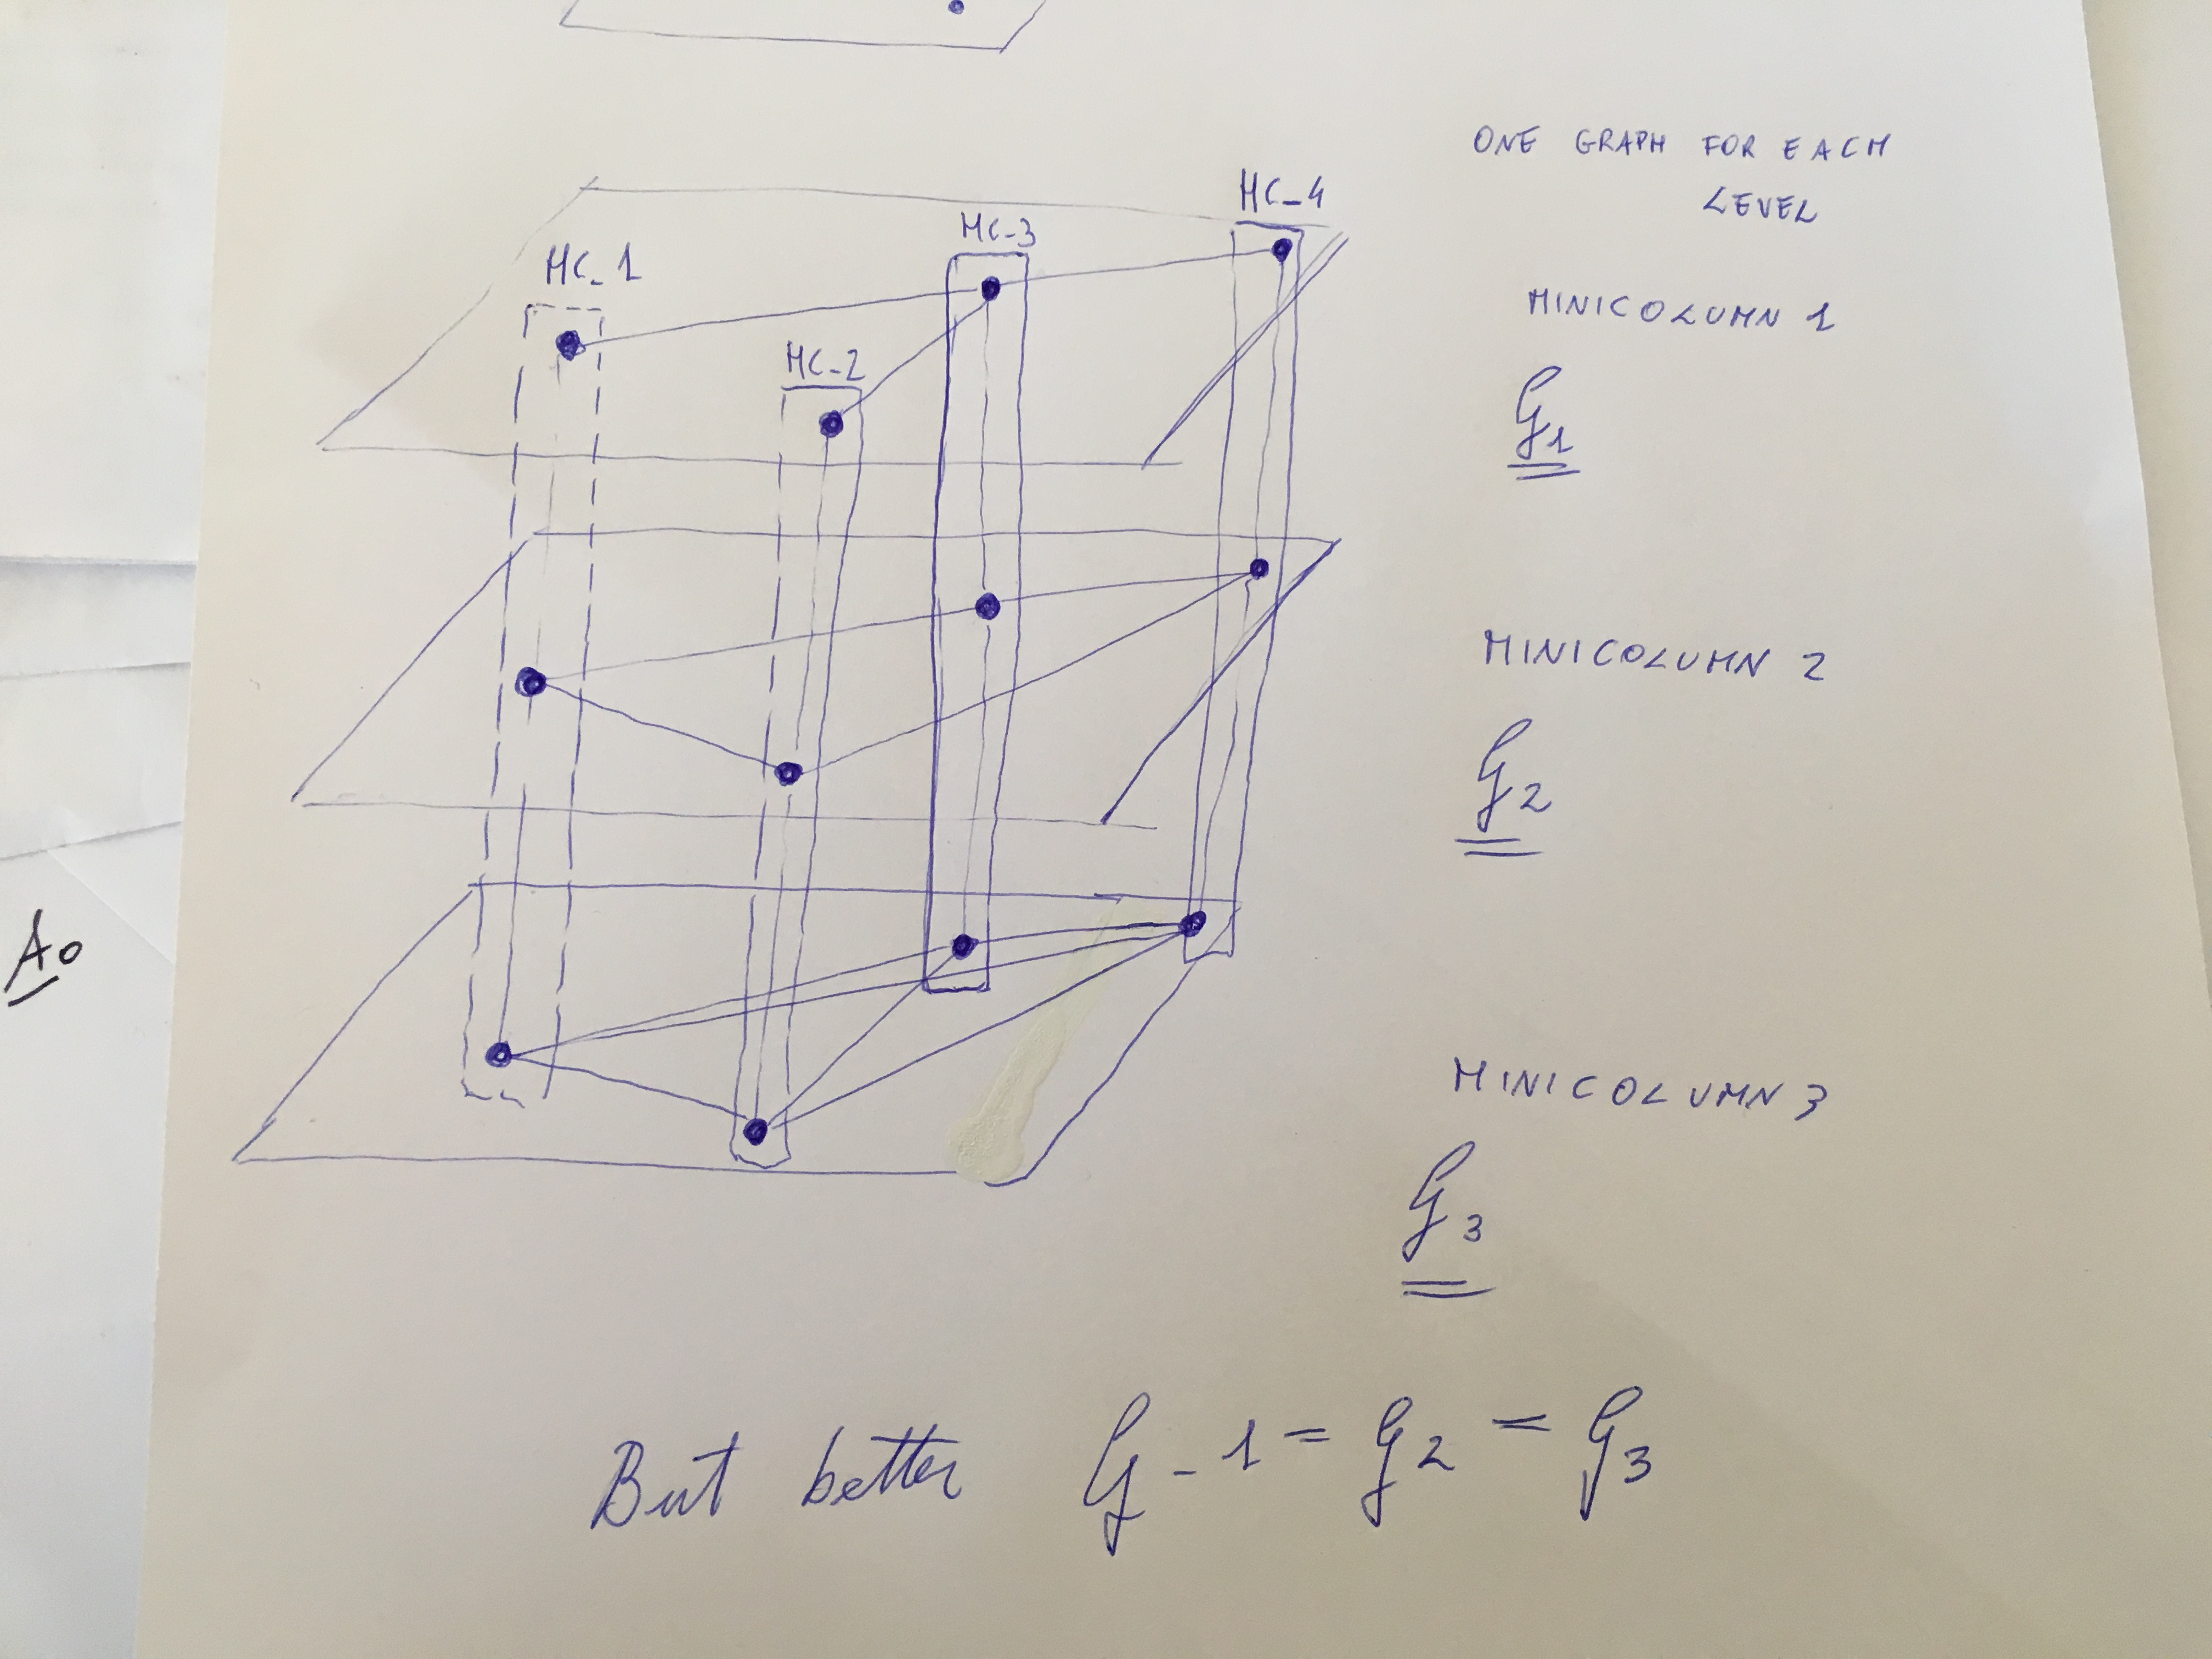
\includegraphics[width=\textwidth]{text/analysis/fig/2by2adapt/image1.jpeg}
    \caption{Simulation of system in \eqref{eq:cl_loop} with several initial conditions. $\alpha=1.5$}
    \label{fig:network_levels}
\end{figure}

\iffalse
\subsection{2by2 system without adaptation}
In this section we consider the dynamics of two interacting hypercolumns, each one made of two minicolumns. The model considered is the rBCPNN in \cref{rBCPNN}. In particular we investigate how the symmetric, mutual interaction between the two modular units, together with the self excitation, shape the qualitative behaviour of the system. We will assume the coupling  weights to be static, result of a previous learning experience. This first analysis heavily exploits the properties of Monotone Control Systems as introduced in \cite{angeli2003monotone} and in particular the reduction theorem proposed in \cite{enciso2005monotone}. We will show how the interaction matrices learned with the Hebbian learning rule make the system monotone according to the right choice of cones and orthants (refer to the Preliminaries section). Furthermore the monotonicity approach will be compared with the Lyapunov Stability approach.

\subsection{Monotonicity Analysis}
Denote $s_{11}, s_{12}, s_{21}, s_{22}$ the activities of the minicolumns grouped into two hypercolumns $s_1 = [s_{11}, s_{12}]^T$ and $s_2 = [s_{21}, s_{22}]^T$;  $o_1 = [o_{11}, o_{12}]^T$ and $o_2 = [o_{21}, o_{22}]^T$ the corresponding outputs computed withe softmax distribution; $\beta_1 = [\beta_{11}, \beta_{12}]$, $\beta_2 = [\beta_{21}, \beta_{22}]$ the self excitation biases; $W$ the interaction matrix between the two units. The interactions are symmetric in the sense that the coupling factor between unit $i$ and unit $j$ is equal to the coupling factor between unit $j$ and unit $i$. The system dynamics follows in the compact form:

\begin{equation}
\begin{aligned}
\tau_m \dot{s_1} &= \beta_{1} + Wo_{2}-s_{1} \\
\tau_m \dot{s_2} &= \beta_{2} + W^{T}o_{1}-s_{2} \\
W & =
\begin{bmatrix}
 w_{1121} & w_{1122} \\
 w_{1221} & w_{1222} \\
\end{bmatrix} = 
\begin{bmatrix}
 w_{1} & w_{2} \\
 w_{3} & w_{4} \\
\end{bmatrix} 
\end{aligned}
\label{eq:cl_loop}
\end{equation}
We can see our system in \eqref{eq:cl_loop} as the closed loop system which arises under unitary output feedback for the following system with input $u$ and output $y$. Given the symmetry of the system, we can choose as output either the output of the hypercolumn $1$ or $2$. Therefore $y=o_1$.

\begin{equation}
\begin{aligned}
\tau_m \dot{s_1} &= \beta_{1} + Wo_{2}-s_{1} \\
\tau_m \dot{s_2} &= \beta_{2} + W^{T}u-s_{2} \\
y & =  o_1
\end{aligned}
\label{eq:op_loop}
\end{equation}

This simple trick will allow us, by using the main result in \cite{enciso2005monotone} to determine the number of asymptotically stable points (attractors) of system in \eqref{eq:cl_loop} by studying a reduced order continuous-time system.

The system in \eqref{eq:op_loop} is a monotone system according to definition [reference to the section in Preliminaries]. In fact ...

Furthermore, we have to show that   the closed loop system in \eqref{eq:cl_loop} is a monotone system with respect to the right choice of orthants (refer to the section on monotone systems). In order to do so we compute the jacobian matrix for the dynamics in \eqref{eq:cl_loop}.
\begin{equation}
\begin{aligned}
\frac{\partial s_{11}}{\partial s_{21}} &= e^{s_{22}} \frac{e^{s_{21}}(w_{1121} - w_{1122}) + w_{1121}e^{s_{22}}    }{e^{s_{21}}(e^{s_{21}}+ e^{s_{22}})} 
\end{aligned}
\label{eq:jac_s1121}
\end{equation}


\begin{equation}
\begin{aligned}
\frac{\partial s_{11}}{\partial s_{22}} &= e^{s_{21}} \frac{e^{s_{22}}(w_{1122} - w_{1121}) + w_{1122}e^{s_{21}}    }{e^{s_{22}}(e^{s_{22}}+ e^{s_{21}})} 
\end{aligned}
\label{eq:jac_s1122}
\end{equation}


\begin{equation}
\begin{aligned}
\frac{\partial s_{12}}{\partial s_{21}} &= e^{s_{22}} \frac{e^{s_{21}}(w_{1221} - w_{1222}) + w_{1221}e^{s_{22}}    }{e^{s_{21}}(e^{s_{21}}+ e^{s_{22}})} 
\end{aligned}
\label{eq:jac_s1221}
\end{equation}


\begin{equation}
\begin{aligned}
\frac{\partial s_{12}}{\partial s_{22}} &= e^{s_{21}} \frac{e^{s_{22}}(w_{1222} - w_{1221}) + w_{1222}e^{s_{21}}    }{e^{s_{22}}(e^{s_{22}}+ e^{s_{21}})} 
\end{aligned}
\label{eq:jac_s1222}
\end{equation}
Analogous results are obtained for $\frac{\partial s_{21}}{\partial s_{11}}, \frac{\partial s_{21}}{\partial s_{12}}, \frac{\partial s_{22}}{\partial s_{11}}, \frac{\partial s_{22}}{\partial s_{12}}$. 

For the following analysis we will assume that during the learning procedure a unique pattern is presented to the network. As explained in (cite section on learning procedure), the pattern is 'fixed' into the network by clamping the input units and leaving the matrix weights adapt. For this first preliminary analysis we will assume that the input current is such that the outputs $o_1 \approx [1 , 0]^T$ and $o_2 \approx [1, 0]^T$. According to \eqref{eq:wij} and assuming that $p_{11} = p_{21} \approx 1$, $p_{12} = p_{22} \approx 0$ a suitable choice for the matrix weights $W$ is the following:  

\begin{equation}
W = \begin{bmatrix}
 0 & -\alpha \\
 -\alpha & 0 \\
\end{bmatrix},\  \alpha = - log(\epsilon) >0
\label{eq:coup_eps_matrix}
\end{equation}
With this particular choice, the partial derivatives above are either strictly positive or negative everywhere in the state space and we can write:

\begin{equation}
\begin{aligned}
\frac{\partial s_{11}}{\partial s_{21}} & > 0, & 
\frac{\partial s_{11}}{\partial s_{22}} & < 0, & \frac{\partial s_{12}}{\partial s_{21}} &< 0, & \frac{\partial s_{12}}{\partial s_{22}}  &> 0
\end{aligned}
\end{equation}

\begin{equation}
\begin{aligned}
\frac{\partial s_{21}}{\partial s_{11}} & > 0, & 
\frac{\partial s_{21}}{\partial s_{22}} & < 0, & \frac{\partial s_{22}}{\partial s_{11}} &< 0, & \frac{\partial s_{22}}{\partial s_{12}}  &> 0
\end{aligned}
\end{equation}
By considering the partial order $\succeq$ induced on ${\rm I\!R}^4$ by the orthant $K = {\rm I\!R}_{\geq 0} \times {\rm I\!R}_{\leq 0} \times {\rm I\!R}_{\geq 0} \times {\rm I\!R}_{\leq 0}$ and by using (link to the right proposition) it follows that the closed loop in \eqref{eq:cl_loop} is a monotone system. An alternative way to show that a system is monotone is to use the graphical conditions for monotonicity developed in \cite{angeli2004multigraph} recalled in the preliminaries section. In particular one need to show that the adjacency matrix describing the sign of the interactions between the states has no negative loops.

\paragraph{Reduced order system} 
Consider now the controlled system in \eqref{eq:op_loop}. By fixing the input $u = [u_1, u_2]^T$ the system converges to the equilibrium point that define  the I/S characteristic $k^X: U \mapsto X$:

\begin{equation}
    \begin{aligned}
    s_1^* &=  \beta_1 + W\sigma(s_2^*)\\
    s_2^* &=  \beta_2 + W^T\sigma(u)\\
    \end{aligned}
\end{equation}
By composing the I/S characteristic with the output function in \eqref{eq:cl_loop} we obtain the I/O characteristic:
\begin{equation}
    k(u) = \sigma(\beta_1 + W\sigma(W^Tu + \beta_2))
    \label{eq:reduced_2d}
\end{equation}
We can now study the following reduced order dynamics:
\begin{equation}
    \dot{u} = k(u) - u
    \label{eq:reduced_2d}
\end{equation}
In this case, the reduced order system is 2-dimensional, therefore a phase plane analysis will help us to understand the nature of equilibrium points. We will first analyse the effect of varying the coupling strength $\alpha$ in the matrix \eqref{eq:coup_eps_matrix}, then the effect of the biases $\beta_1,\beta_2$.

\paragraph{Effect of coupling strength $\alpha$} We study the effect of varying the coupling strength by a phase portrait analysis. The bias parameters $ \beta_1, \beta_2$ are nitially assumed to be zero. In particular we can notice that by increasing the coupling factor $ \alpha $ from 0 (no coupling) to higher values, two stable equilibria emerges \cref{fig:two_d_system_eps_effect}. This is a particular case of \textbf{supercrictical pitchfork bifurcation} \cite{StrogatzNonlinear}: in fact, by varying the parameter $\alpha$, the system transitions from one (stable) fixed point to three fixed points: one unstable and two stable (\cref{fig:two_d_system_eps_effect}). 

Simulations of the original system on \eqref{eq:cl_loop} with different initial conditions show that, as expected, the qualitative behaviour (number of fixed points) of the 2-dimensional reduced order system is kept in the original 4-dimensional system. In \cref{fig:s_mono_one} and \cref{fig:s_mono_two} the evolution of states with several initial conditions, both for $\alpha=1.5$ (one equilibrium) and $\alpha=8$ (2 equilibria) is shown.

\iftrue
   \begin{figure*}
        %\centering
        \begin{subfigure}[b]{0.475\textwidth}
            \centering
            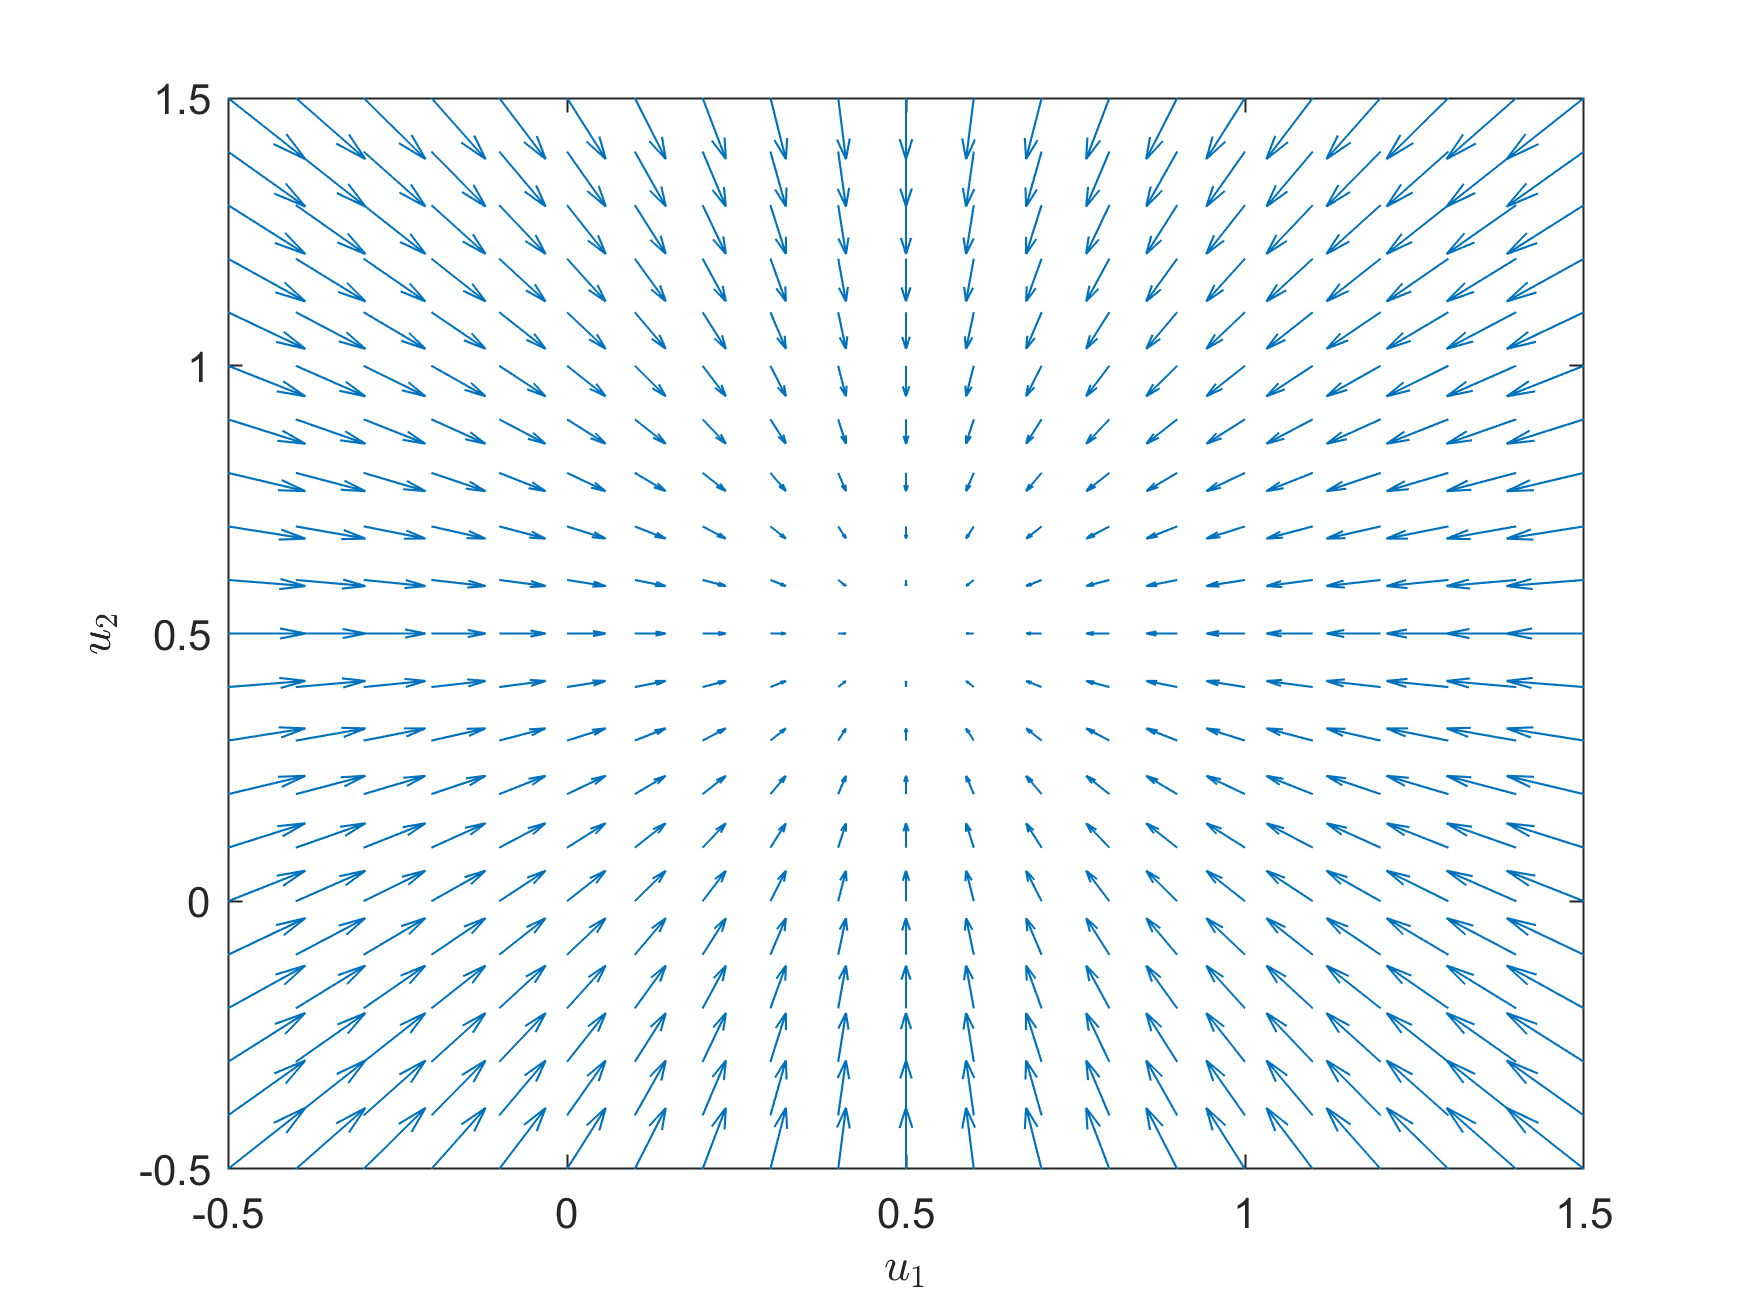
\includegraphics[width=\textwidth]{text/analysis/fig/2by2monotone/espi_0.png}
            \caption{\small $\alpha=0$}
            \label{fig:mean and std of net14}
        \end{subfigure}
        \hfill
        \begin{subfigure}[b]{0.475\textwidth}  
            \centering 
            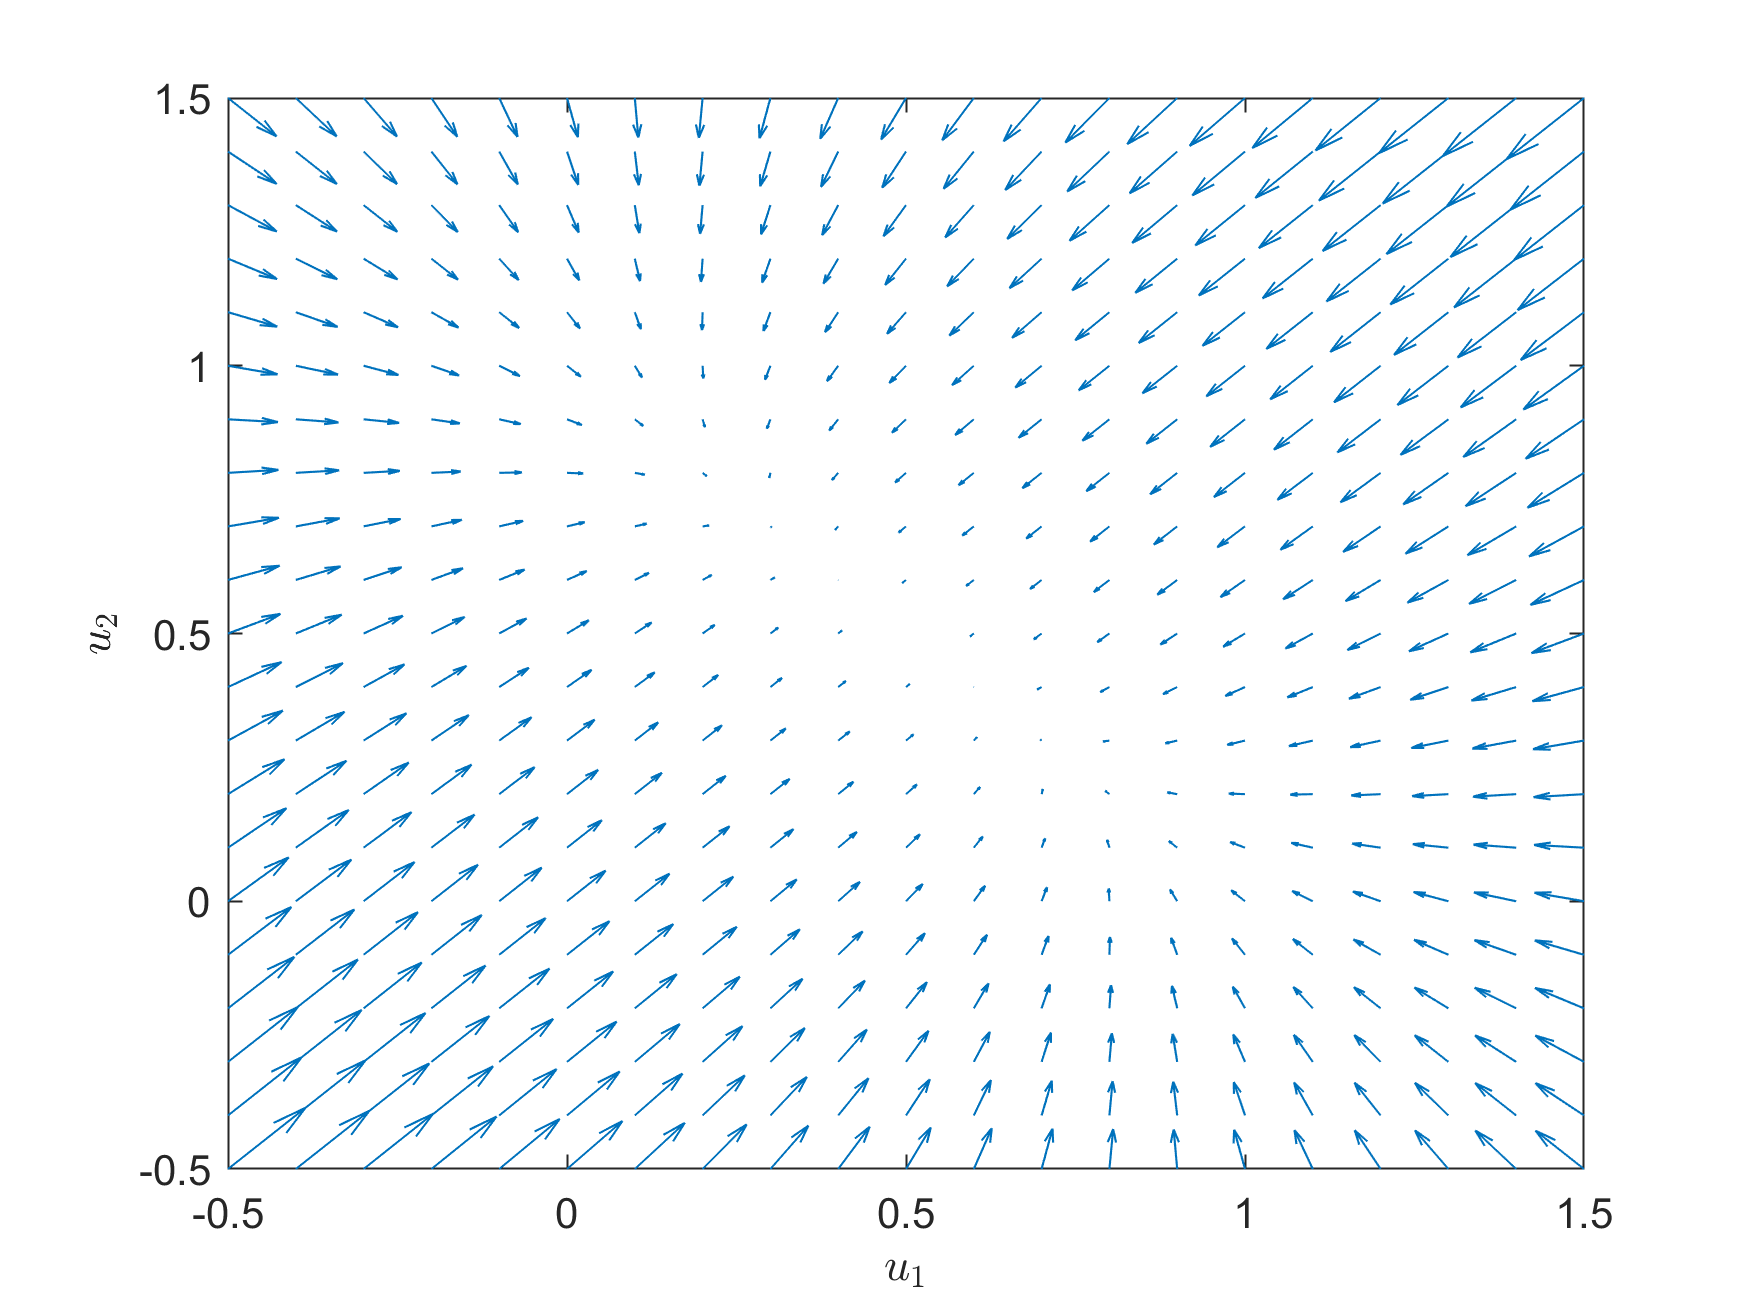
\includegraphics[width=\textwidth]{text/analysis/fig/2by2monotone/espi_2.png}
            \caption{$\alpha=2$}
            \label{fig:mean and std of net24}
        \end{subfigure}
        \vskip\baselineskip
        \begin{subfigure}[b]{0.475\textwidth}   
            \centering 
            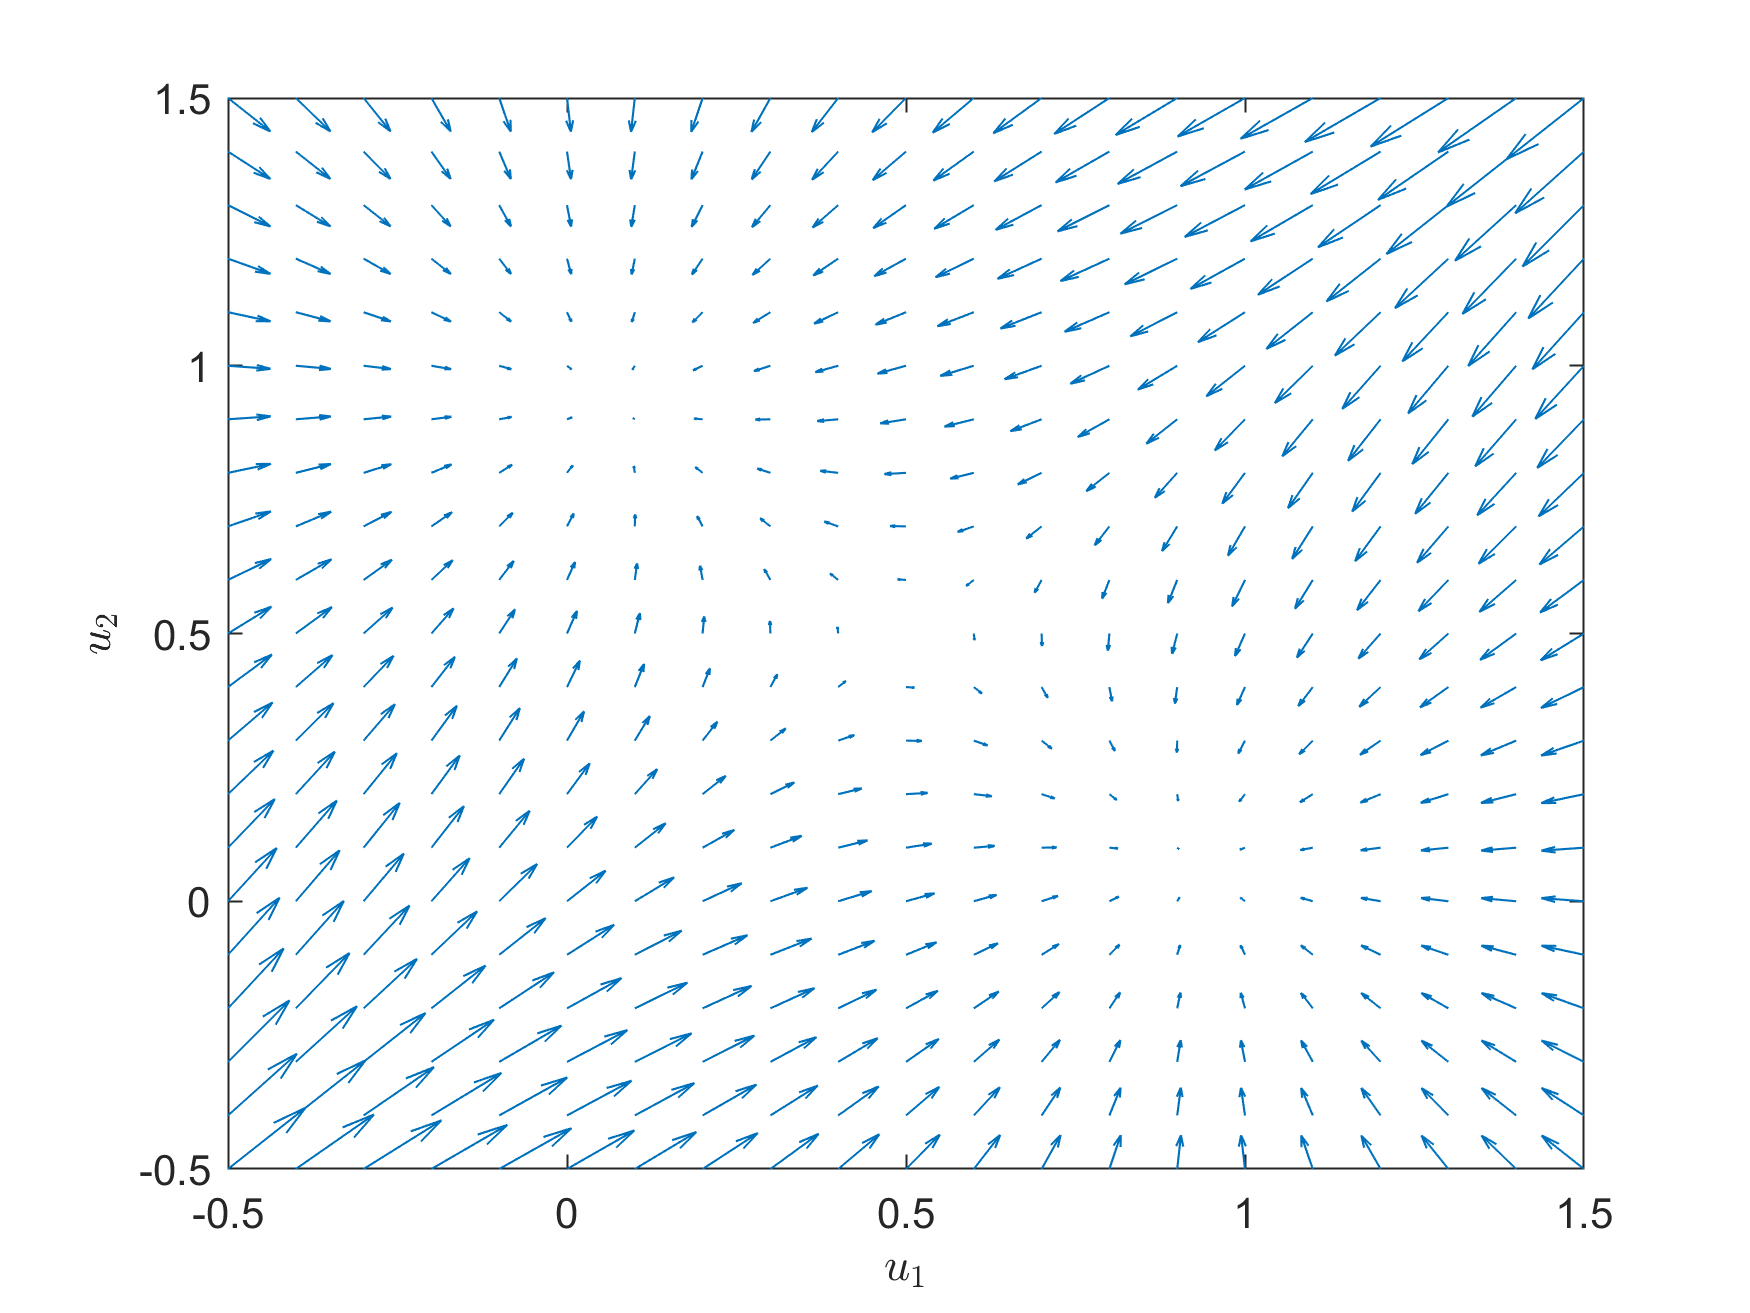
\includegraphics[width=\textwidth]{text/analysis/fig/2by2monotone/espi_3.png}
            \caption{$\alpha=3$}
            \label{fig:mean and std of net34}
        \end{subfigure}
        \quad
        \begin{subfigure}[b]{0.475\textwidth}   
            \centering 
            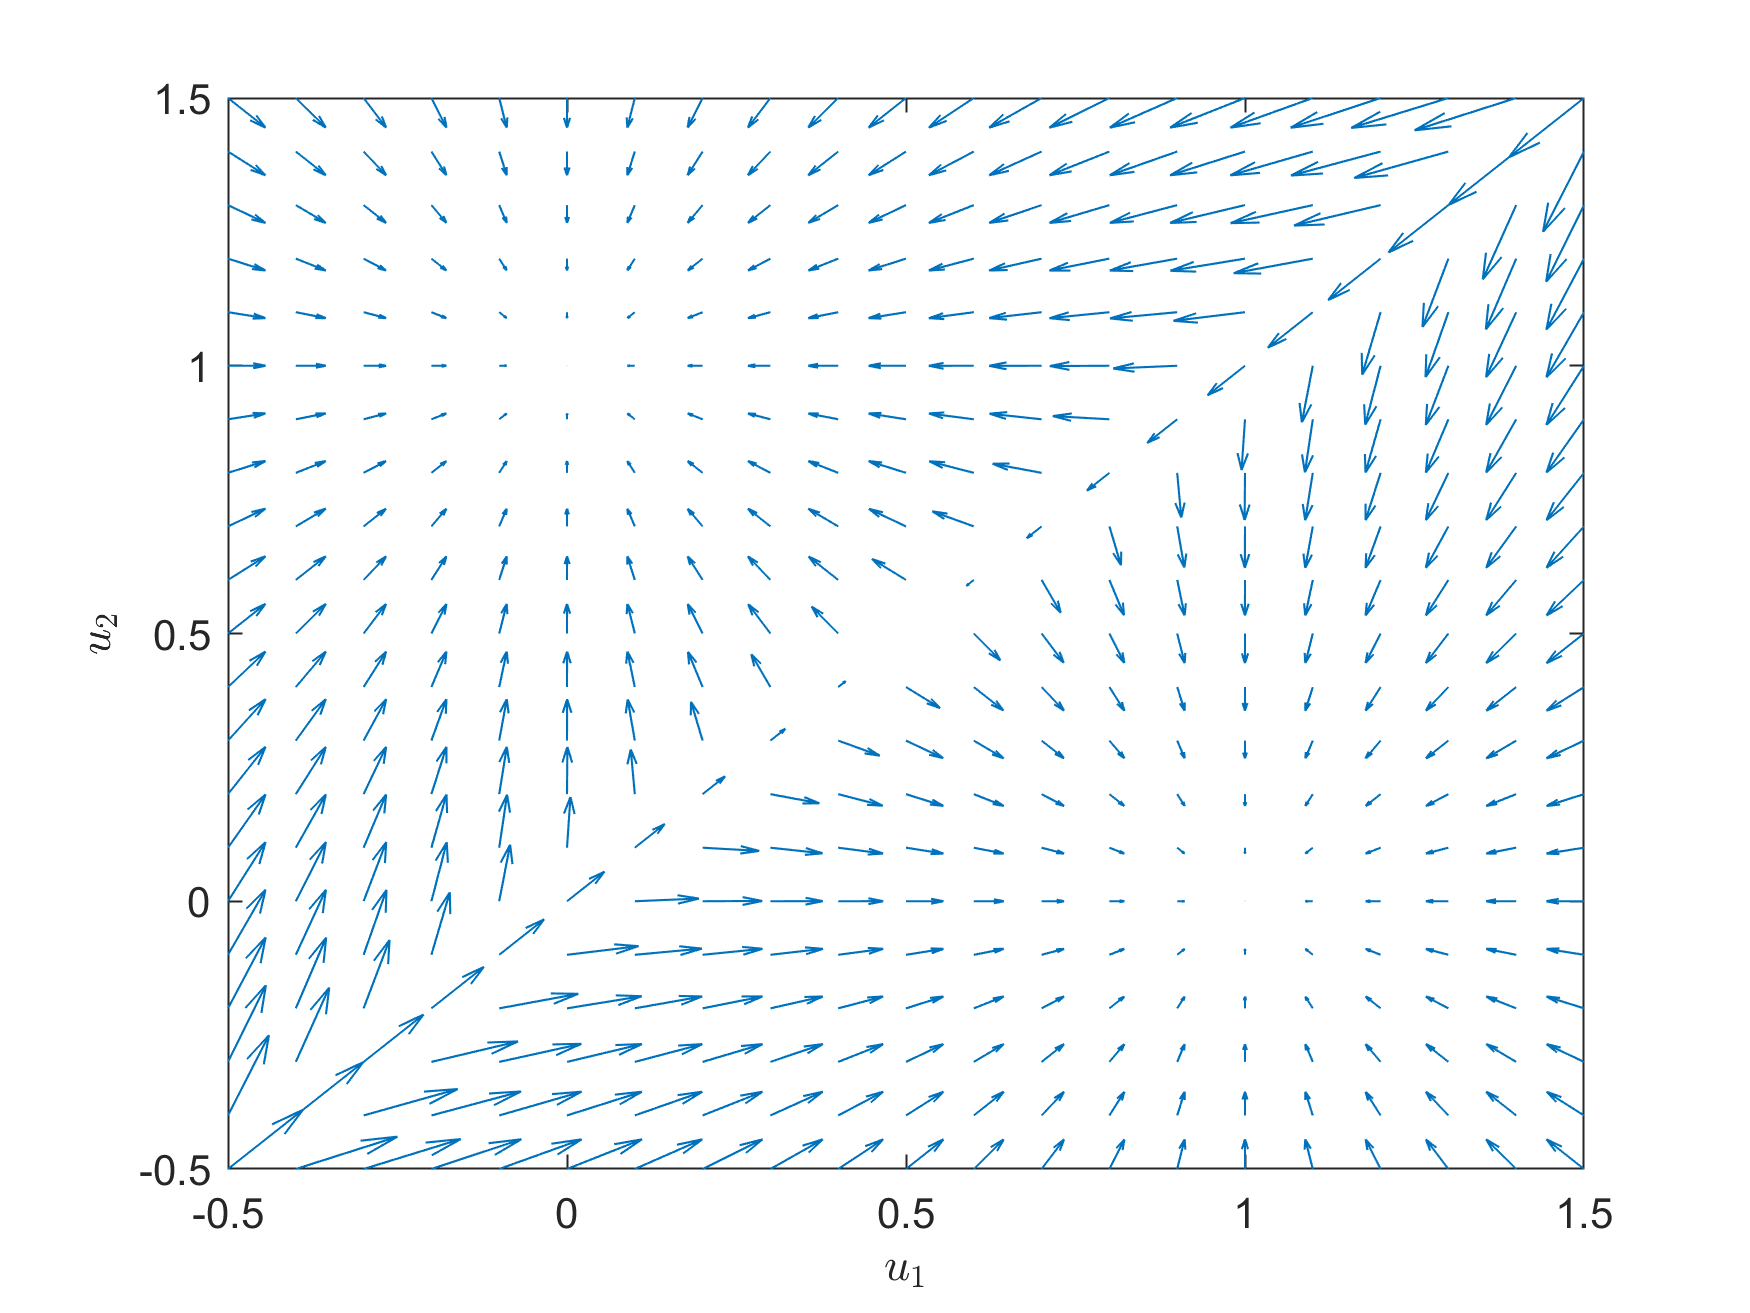
\includegraphics[width=\textwidth]{text/analysis/fig/2by2monotone/espi_8.png}
            \caption{$\alpha=8$}
            \label{fig:mean and std of net44}
        \end{subfigure}
        \caption{Phase portrait for the system in \eqref{eq:reduced_2d} with different coupling factors. $u=[u_1, u_2]^T$} 
        \label{fig:two_d_system_eps_effect}
    \end{figure*}
\fi

\begin{figure}
    \centering
    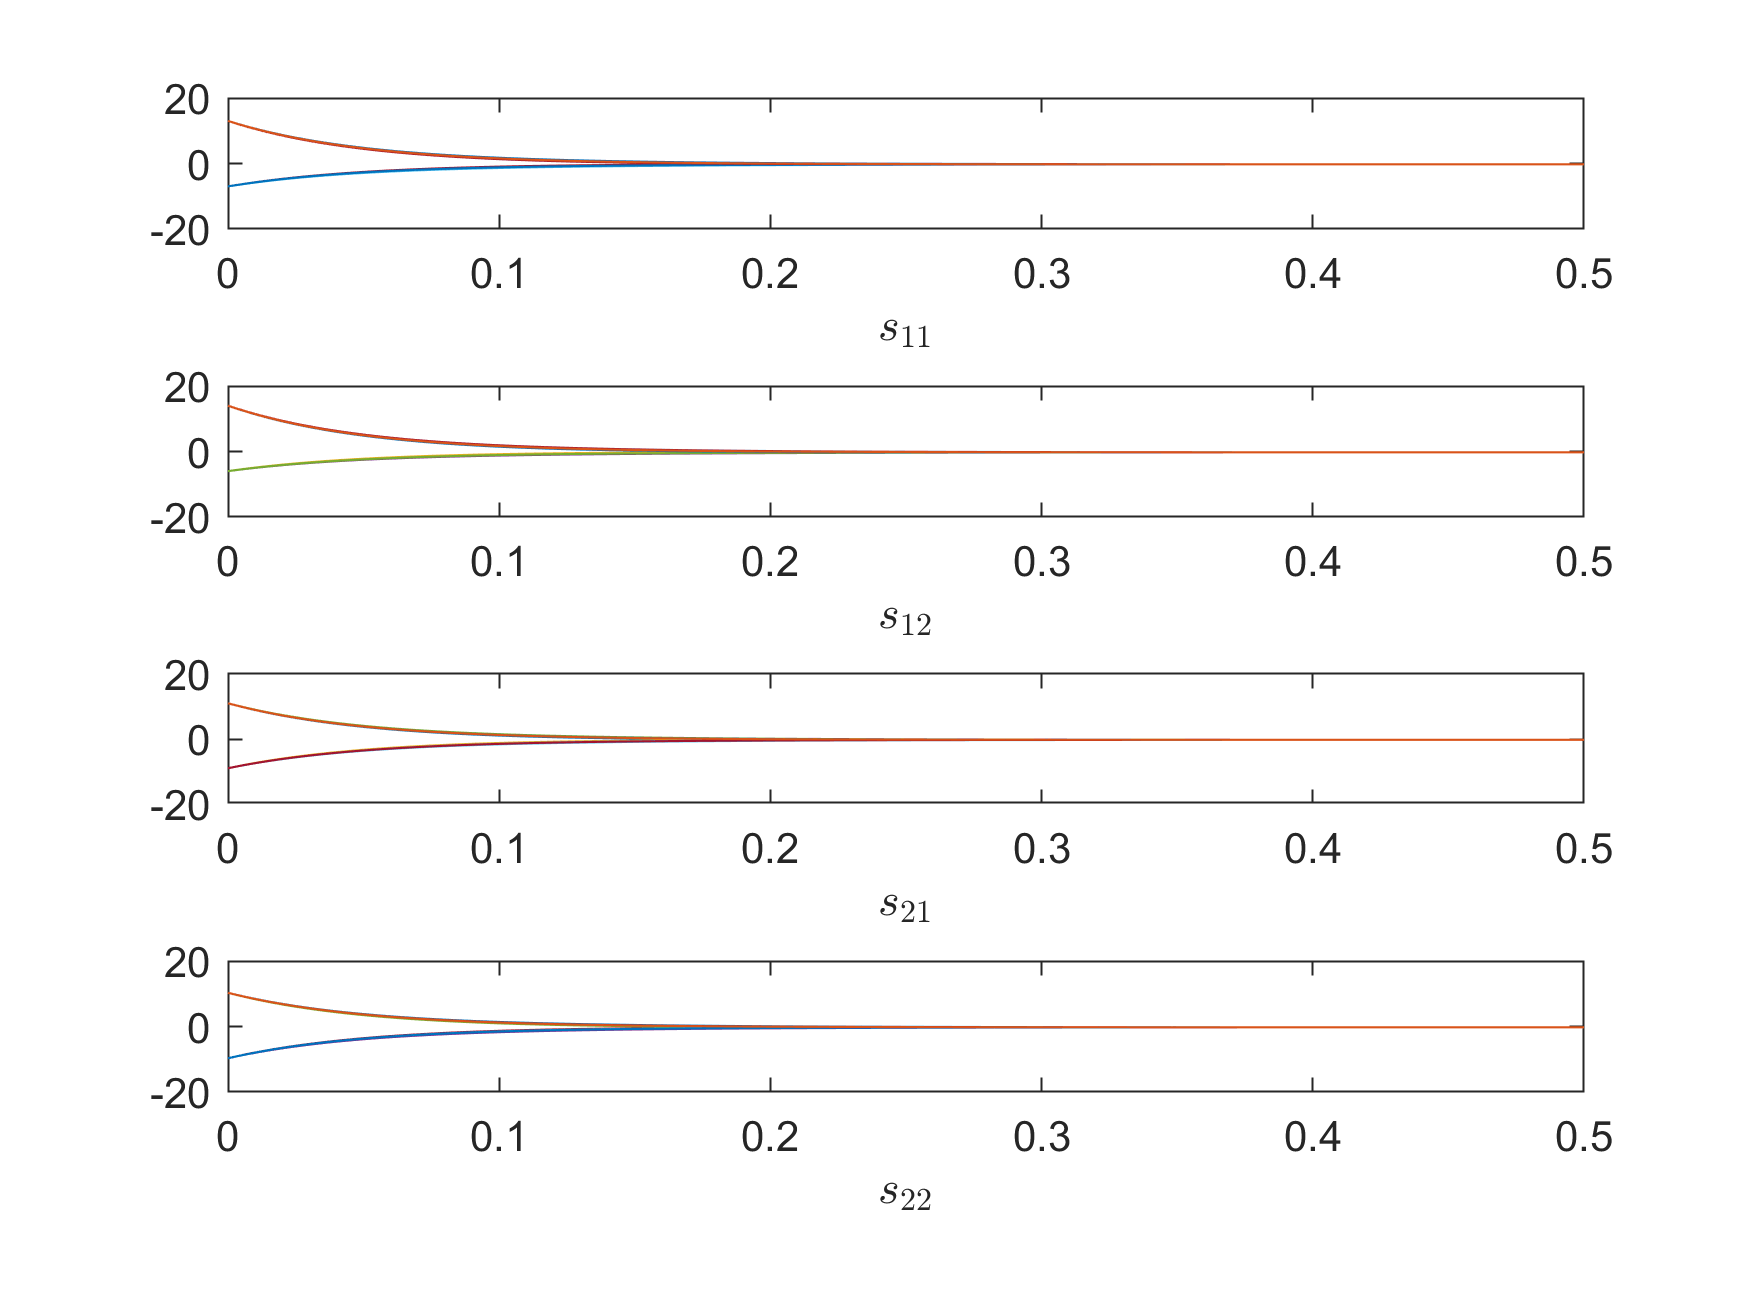
\includegraphics[width=\textwidth]{text/analysis/fig/2by2monotone/s.png}
    \caption{Simulation of system in \eqref{eq:cl_loop} with several initial conditions. $\alpha=1.5$}
    \label{fig:s_mono_one}
\end{figure}
    
\begin{figure}
    \centering
    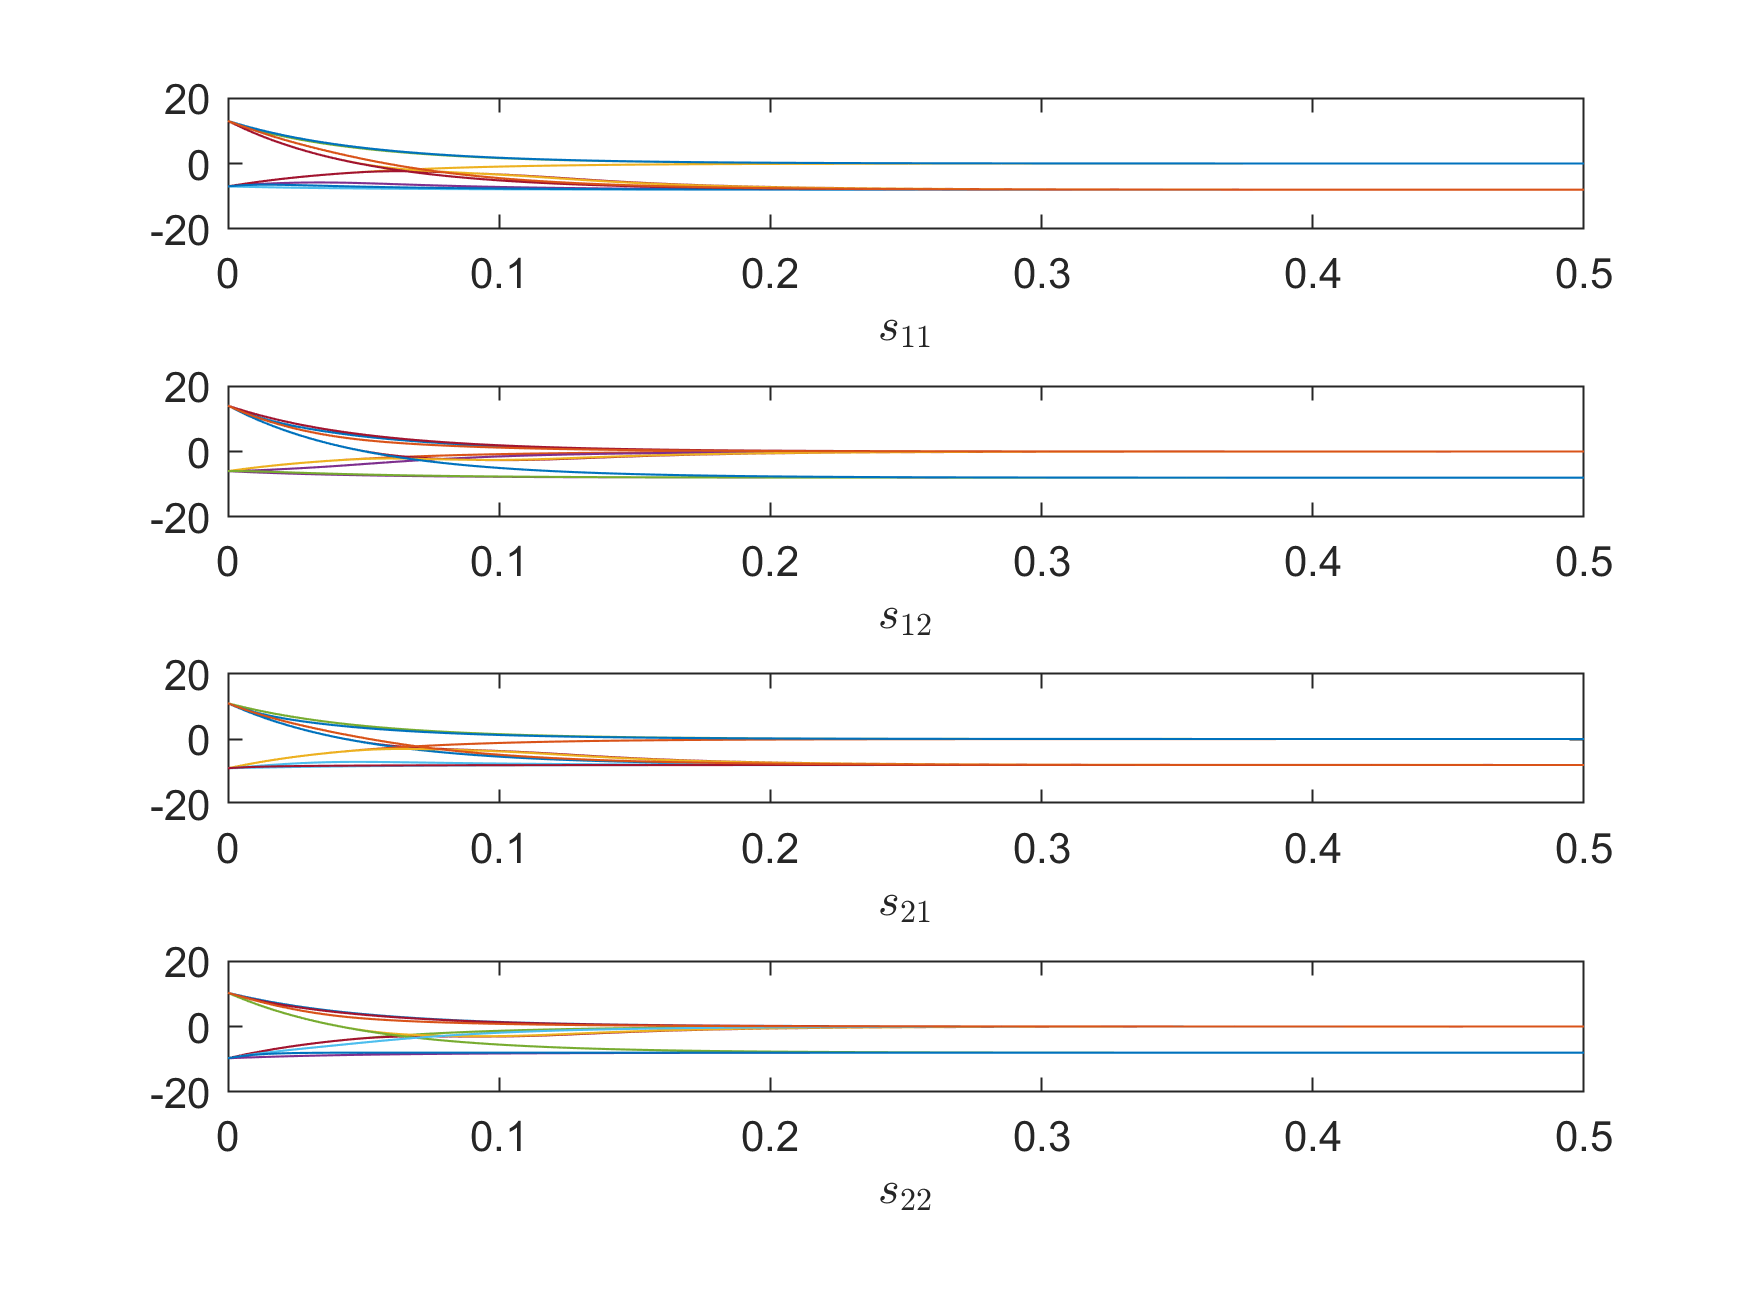
\includegraphics[width=\textwidth]{text/analysis/fig/2by2monotone/s_2.png}
    \caption{Simulation of system in \eqref{eq:cl_loop} with several initial conditions. $\alpha=8$}
    \label{fig:s_mono_two}
\end{figure}
        
    
\paragraph{Effect of biases $\beta$} It is interesting to study the effect of the bias parameters $\beta_1,\beta_2 $ on the number of equilibria and the size of the basin of attraction. In particular, we will consider the effect of the biases both for $\alpha<\alpha^* $ and also for $\alpha>\alpha^* $ (system with coupling above bifurcation threshold). 

When $\alpha<\alpha^*$ changing the bias parameters $\beta_1, \beta_2$ does not affect the qualitative behaviour of the system. In fact, the only effect is the one of changing the position of the attractor of the state space.

When $\alpha>\alpha^*$ changing the bias parameters $\beta_1, \beta_2$ moves the equilibria in such a way that a \textbf{saddle-node bifurcation} occurs.
Since the original system in \eqref{eq:cl_loop} is symmetric with respect to the choice of $s_1$ or $s_2$ we can study the effect of changing the bias terms by studying $\beta_2$ and keeping constant $\beta_1$. Furthermore, varying both $\beta_{21}$ and $\beta_{22}$ is not particularly interesting since what determines the behaviour of the system is the difference  $\beta_{21} - \beta_{22}$. Therefore, for simplicity we are gonna study the effect of varying the bias $\beta_{21}$ and keeping $\beta_{22}$ fixed. 

Increasing $\beta_{21}$ (in a neurobiological framework this corresponds to a higher level of self-excitation) the basin of attraction corresponding to the equilibrium $(1, 0)$ expands until a \textbf{saddle-node bifurcation} occurs (refer to section in the preliminaries). This can be intuitively interpreted as follows: by increasing the self-activation of one unit, the basin of attraction corresponding to the pattern in which the corresponding unit is active expands at the expenses of the other attractors until they eventually get completely 'adsorbed'. In \cref{fig:two_d_system_bias_effect} this effect is visible with the help of the phase portrait analysis.

\iftrue
   \begin{figure*}
        %\centering
        \begin{subfigure}[b]{0.475\textwidth}
            \centering
            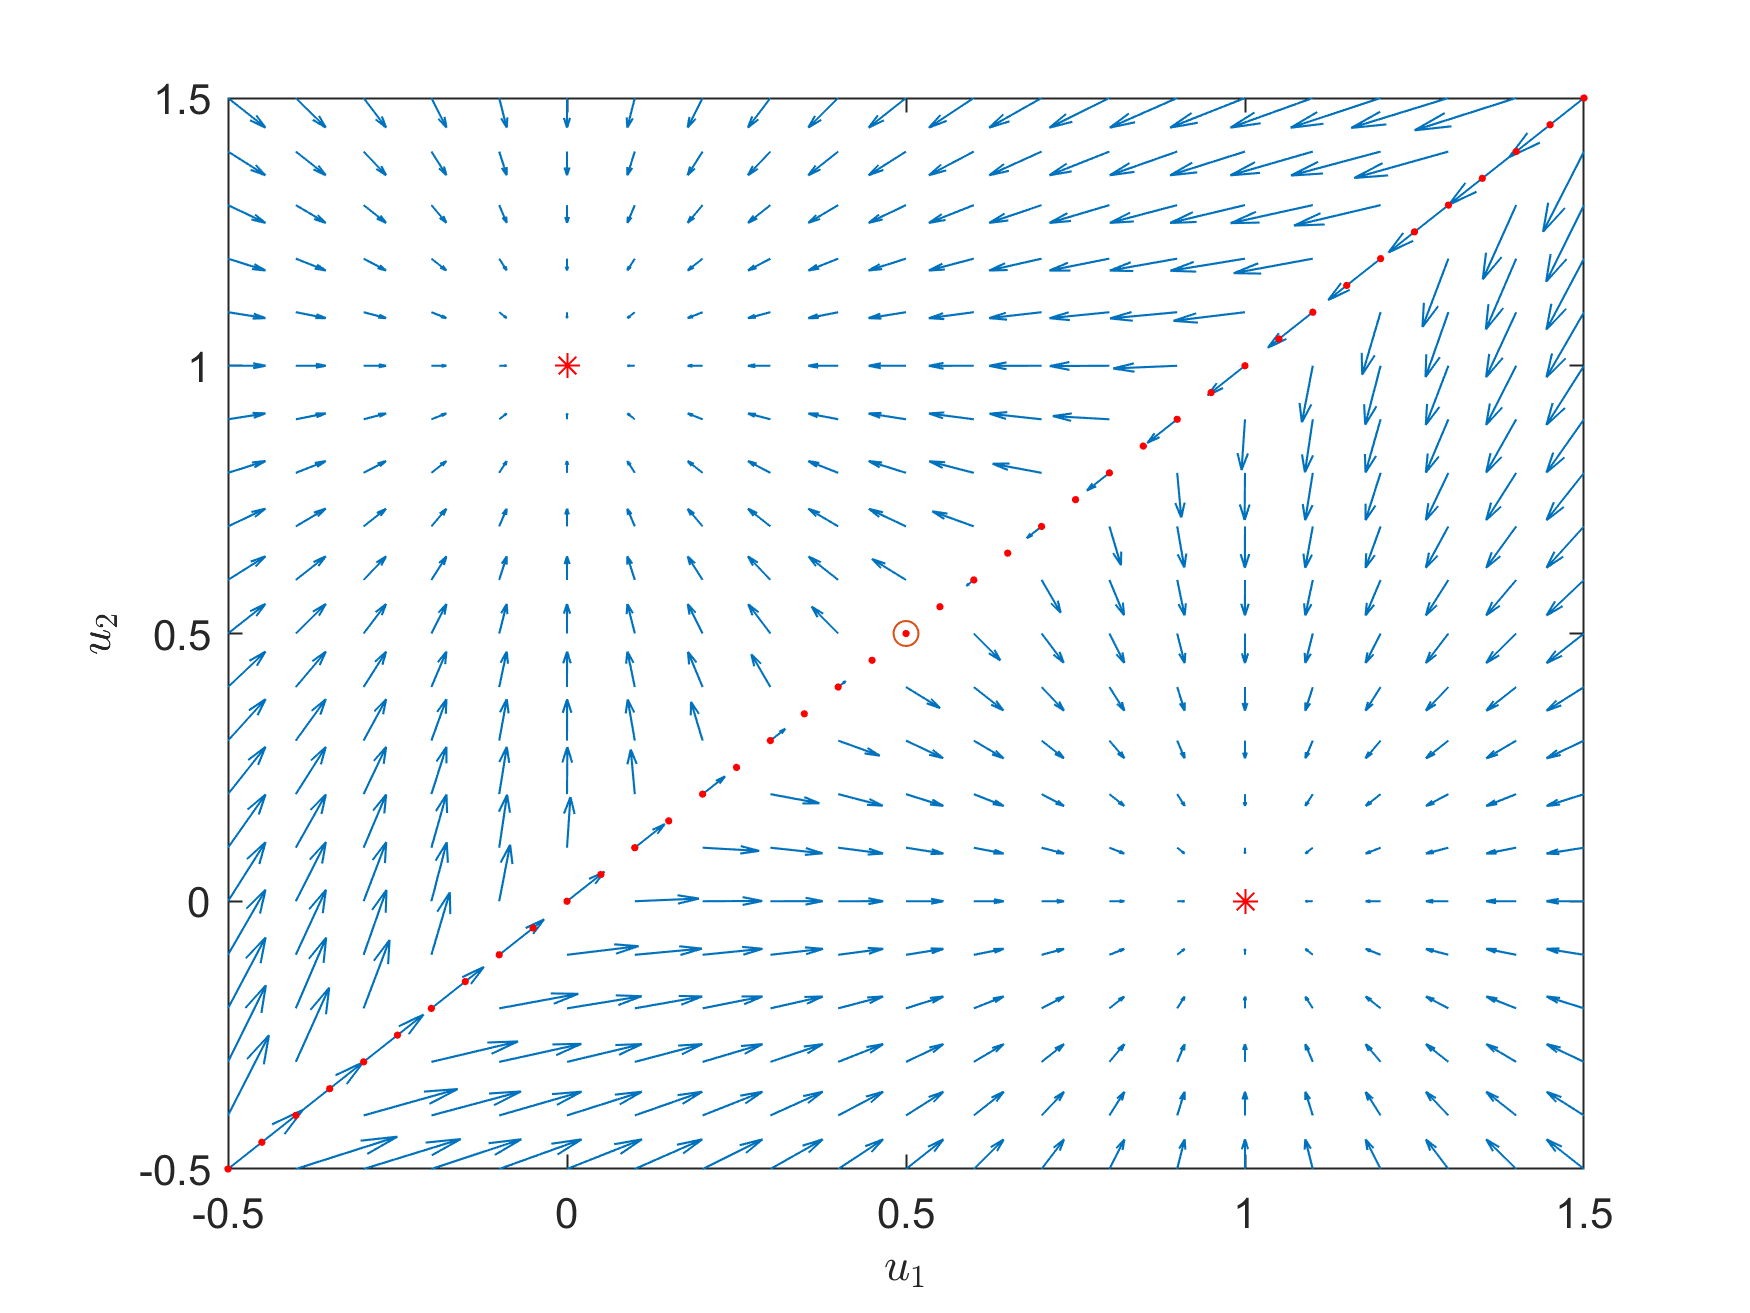
\includegraphics[width=\textwidth]{text/analysis/fig/2by2monotone/bias_0.png}
            \caption{\small $\beta_{21}=0$}
            \label{fig:mean and std of net14}
        \end{subfigure}
        \hfill
        \begin{subfigure}[b]{0.475\textwidth}  
            \centering 
            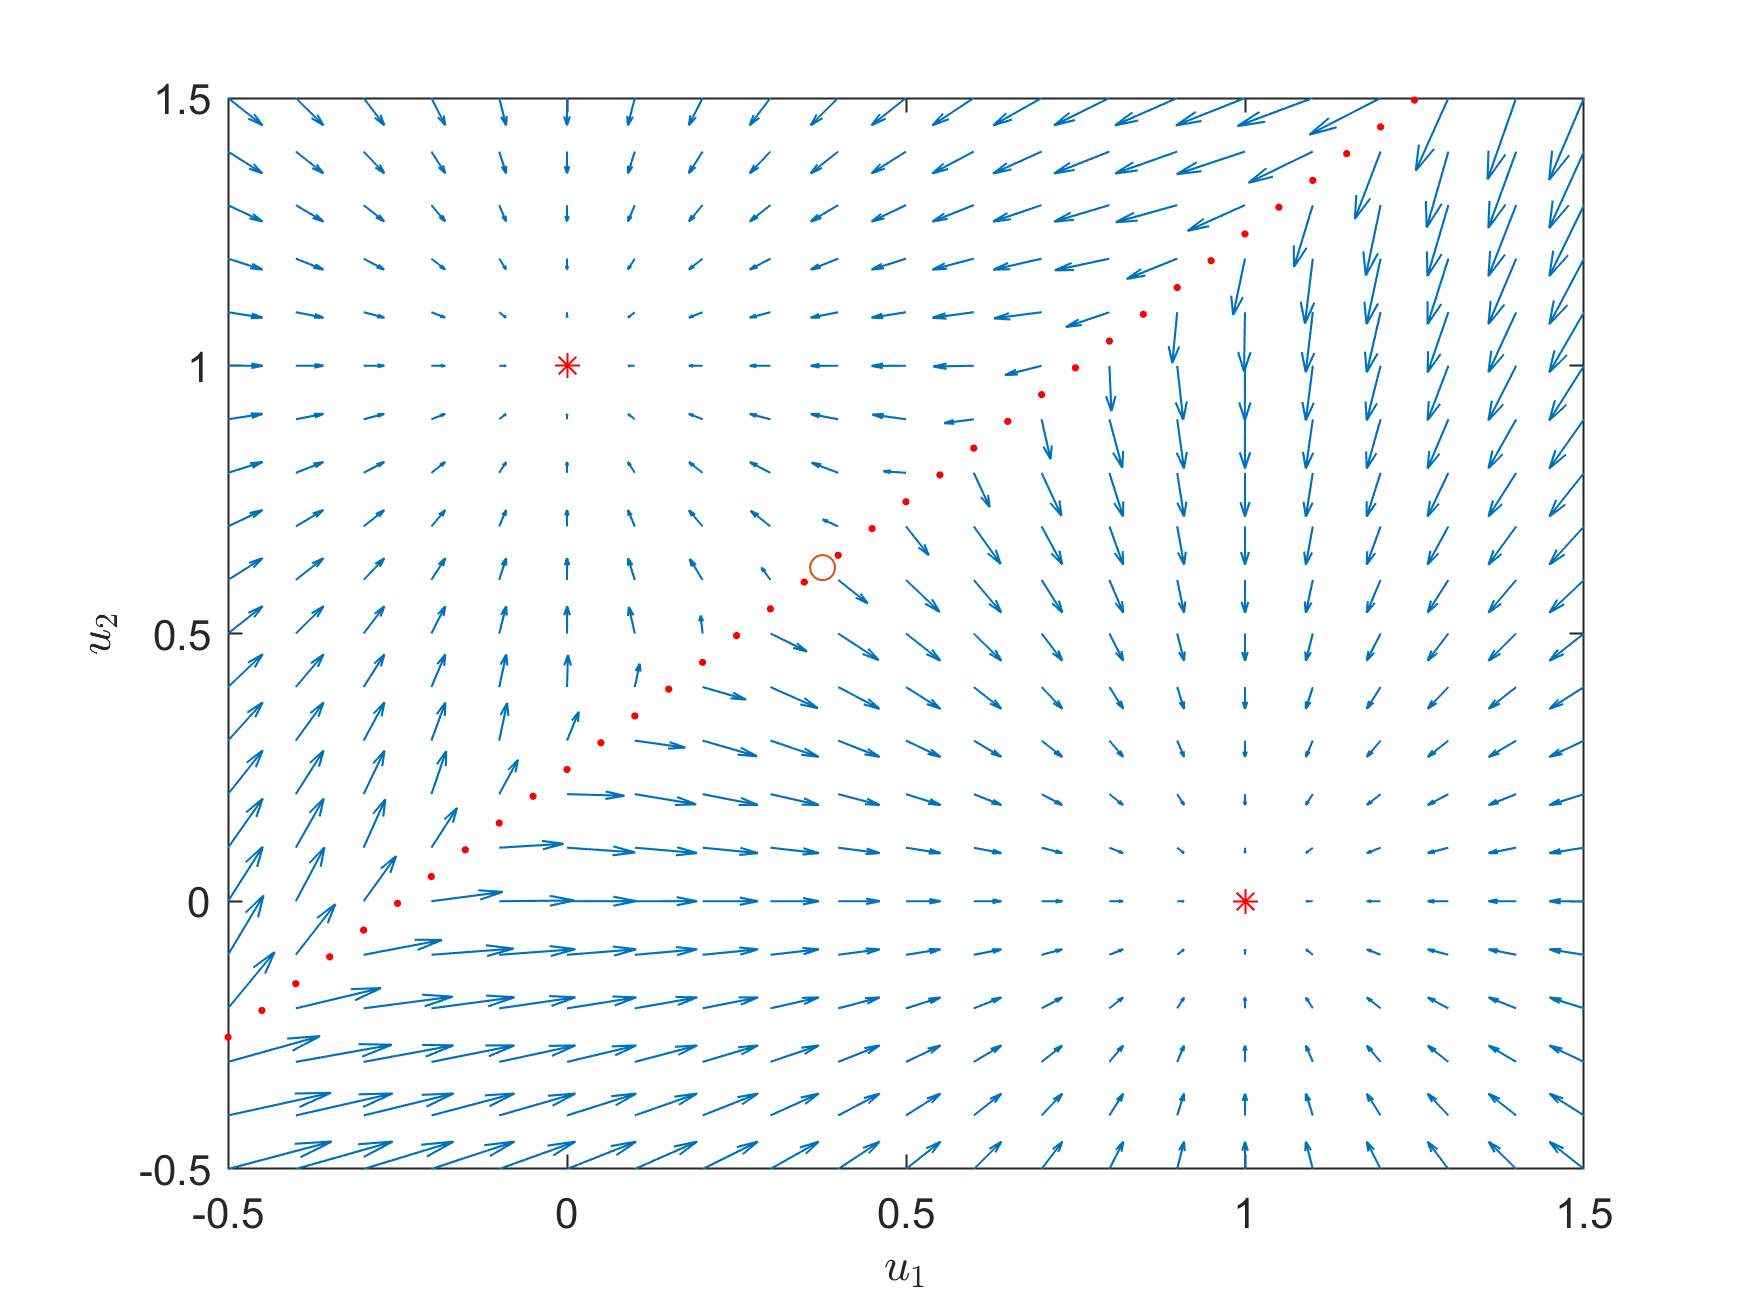
\includegraphics[width=\textwidth]{text/analysis/fig/2by2monotone/bias_2.png}
            \caption{$\beta_{21}=2$}
            \label{fig:mean and std of net24}
        \end{subfigure}
        \vskip\baselineskip
        \begin{subfigure}[b]{0.475\textwidth}   
            \centering 
            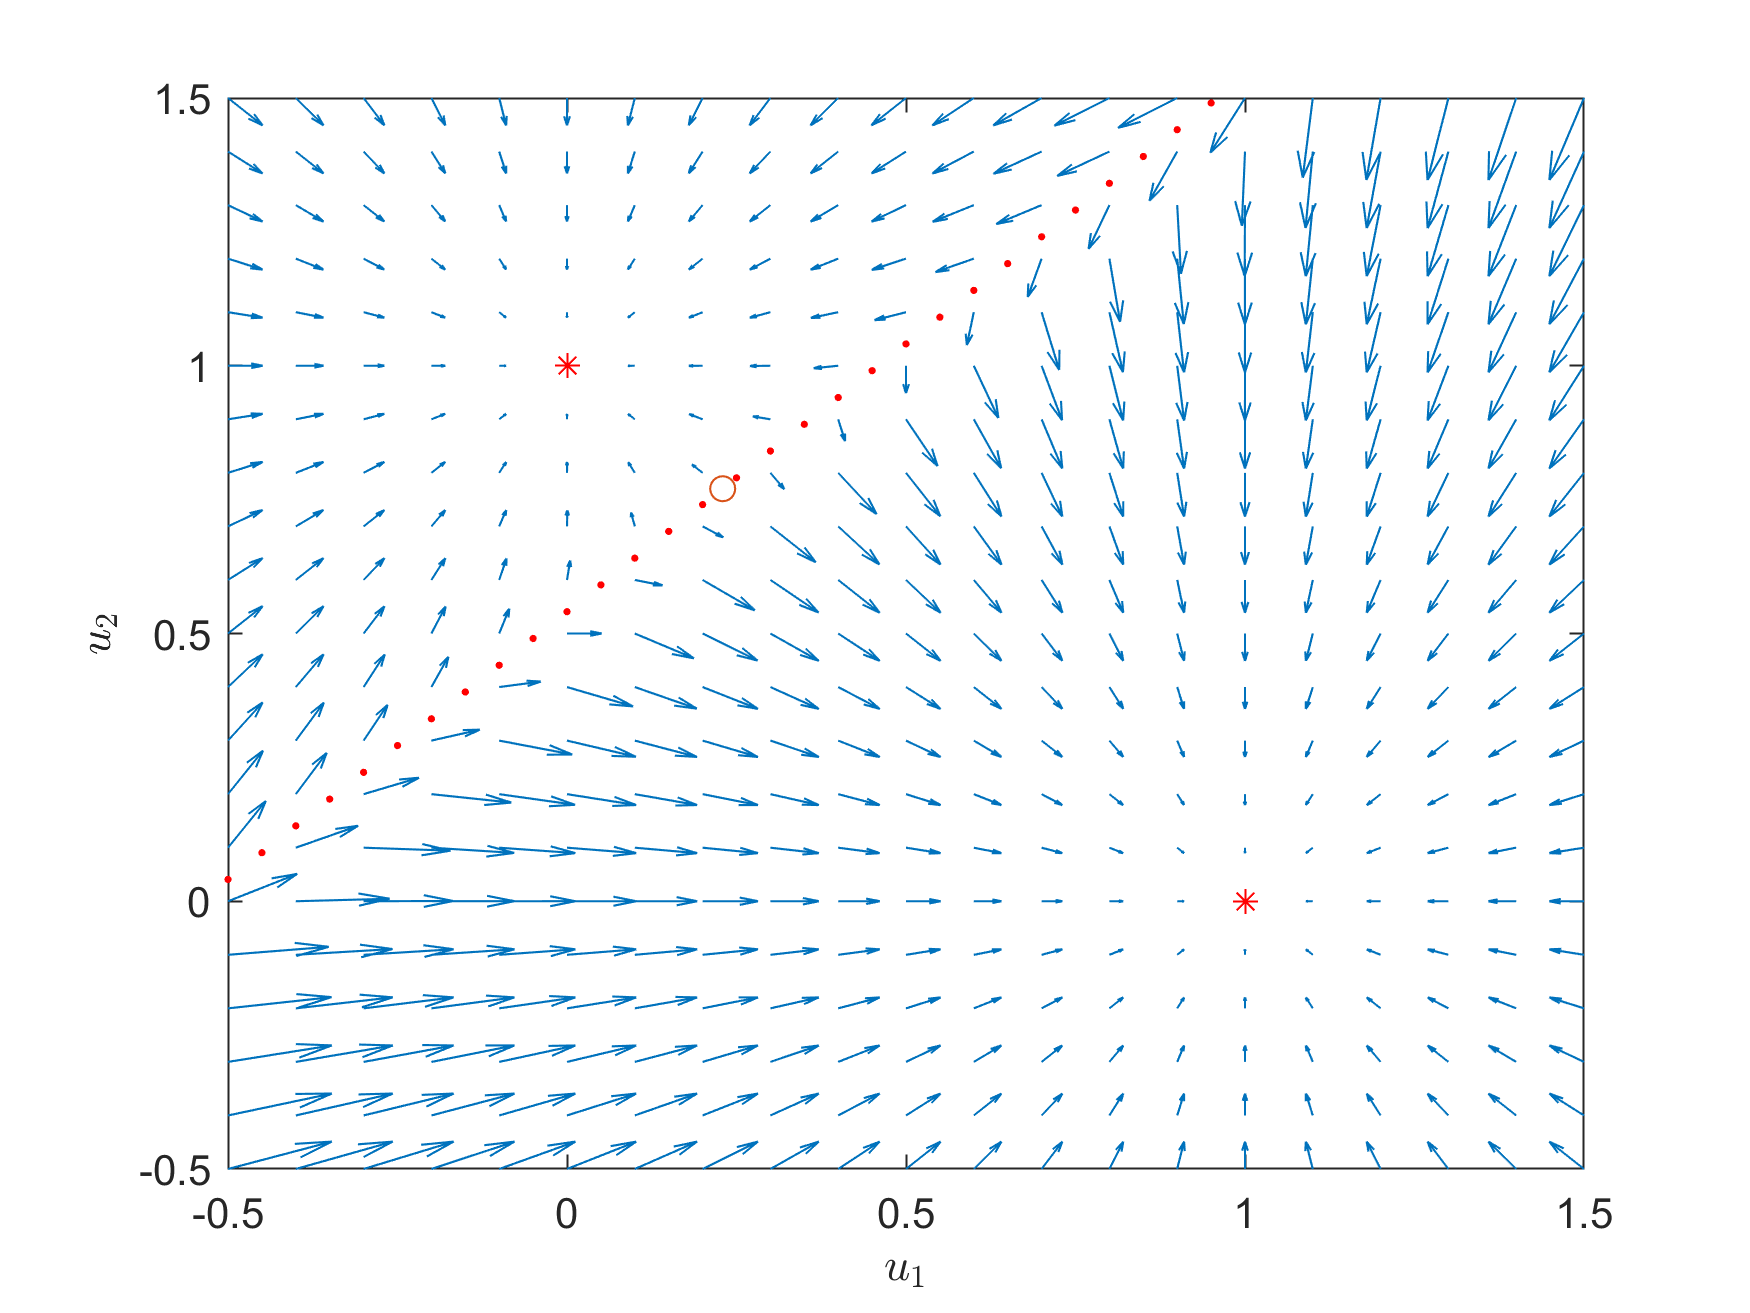
\includegraphics[width=\textwidth]{text/analysis/fig/2by2monotone/bias_4.png}
            \caption{$\beta_{21}=4$}
            \label{fig:mean and std of net34}
        \end{subfigure}
        \quad
        \begin{subfigure}[b]{0.475\textwidth}   
            \centering 
            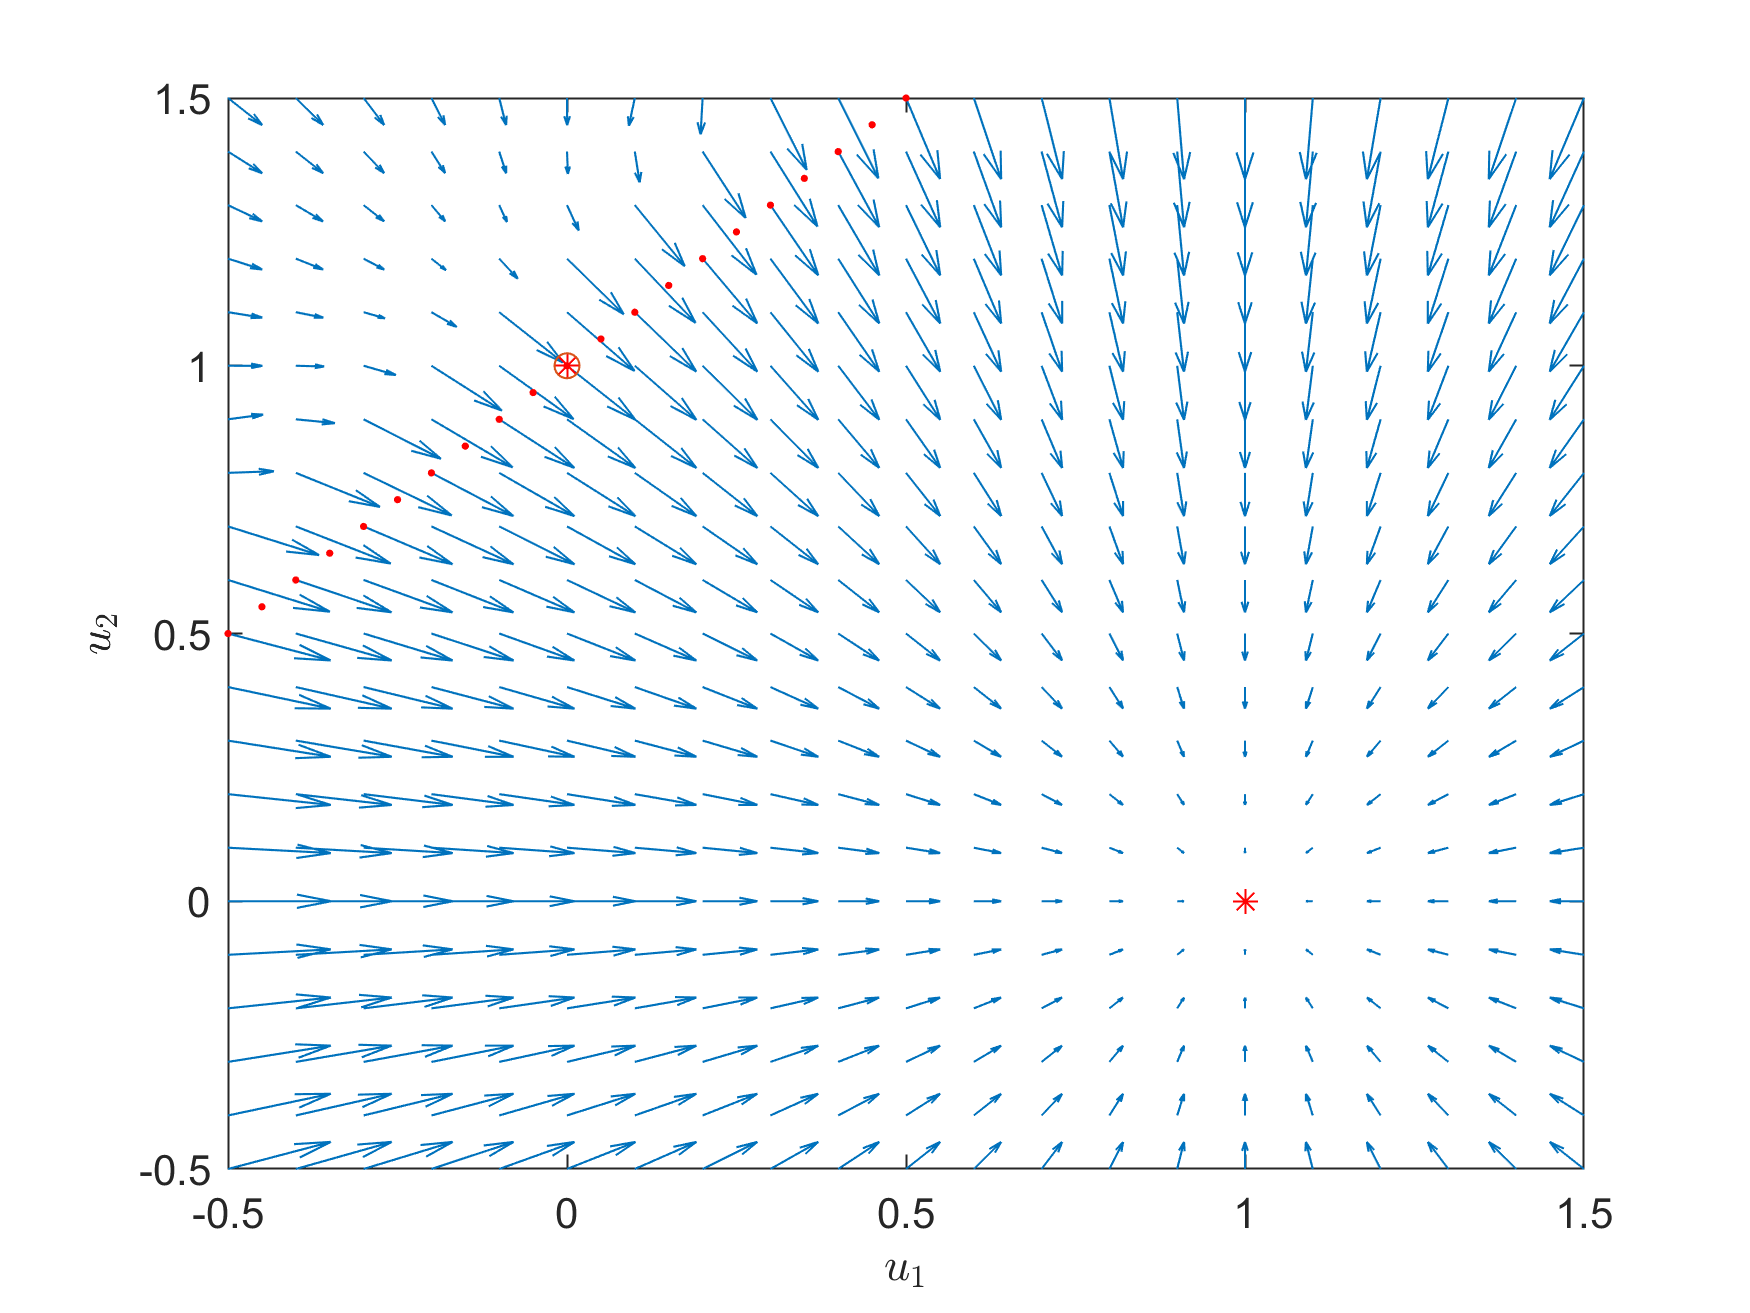
\includegraphics[width=\textwidth]{text/analysis/fig/2by2monotone/bias_10.png}
            \caption{$\beta_{21}=10$}
            \label{fig:mean and std of net44}
        \end{subfigure}
        \caption{Phase portrait for the system in \eqref{eq:reduced_2d} with different coupling factors. $u=[u_1, u_2]^T$} 
        \label{fig:two_d_system_bias_effect}
    \end{figure*}
\fi

\paragraph{Limitations} We have seen so far how the Monotonicity analysis of this section helped us to reduce the complexity of our 4-dimensional system, allowing us to study a 2-dimensional system. Furthermore, we got some interesting insight on the role of the dynamics parameters $\alpha$ and $\beta$. Unfortunately, this approach can not be easily extended to a system with a higher number of dimensions and can not be applied to a system with negative loops as we will see when we will add the adaptation module.
\fi
\subsection{4-dimensional uncoupled oscillator}
%In this section we analyse the effect of the adaptation module on the behaviour of the system. As already discussed in previous works (\cite{sandberg2002bayesian} for example), the role of adaptation is related with the presence of oscillations (sequential reactivation of the different patterns stored into the network). In the adopted model \cite{LansnerFRC} the adaptation acts as a local relaxation of the single minicolumns activity. 
 
 We will first focus on a system made by two hyper-columns each one made of 2 minicolumns interacting via their outputs.
 
 \paragraph{Assumptions}
 The assumptions presented below are kept fixed for the analysis that follows in this section:
 \begin{itemize}
     \item \textbf{A1} The matrix $W$ that describes the coupling of the units in the system is fixed, shaped by a previous learning experience.
     \item \textbf{A2} The coupling matrix is a diagonal matrix $W = \epsilon  I_{2}$ where $I_{2}$ is the 2-dimensional identity matrix. This choice corresponds to two stored orthogonal memory patterns. The parameter $\epsilon$ is a positive constant that parametrizes the coupling strength between the units. For simplicity in the notation the identity matrix will be written as $I$ without expliciting the dimension.
     \item \textbf{A3} The adaptation has a slower dynamics with respect to the activity dynamics of the minicolumns, therefore $\tau_a > 1$
 \end{itemize}
 
 \paragraph{System equations}
 Before going further with the analysis of the system with adaptation we recall the system's dynamics.
 
Denote $s_{11}, s_{12}, s_{21}, s_{22}$ the activities of the minicolumns grouped in the two hyper-columns $s_1 = [s_{11}, s_{12}]^T$ and $s_2 = [s_{21}, s_{22}]^T$;  $o_1 = [o_{11}, o_{12}]^T$ and $o_2 = [o_{21}, o_{22}]^T$ the corresponding outputs computed with the soft-max distribution; $W=\varepsilon I, \epsilon>0$ the interaction matrix between the two units. The interactions are symmetric in the sense that the coupling factor between unit $i$ and unit $j$ is equal to the coupling factor between unit $j$ and unit $i$.  The system dynamics follows:
\begin{equation}
\begin{aligned}
    \dot{s}_{11}&=-s_{11}-a_{11}+\varepsilon I o_{21} \\
    \tau_a \dot{a}_{11}&=g_a o_{11} - a_{11} \\
    \dot{s}_{12}&=-s_{12}-a_{12}+\varepsilon I o_{22} \\
    \tau_a \dot{a}_{12}&=g_a o_{12} - a_{12} \\
    \dot{s}_{21}&=-s_{21}-a_{21}+\varepsilon I o_{11} \\
    \tau_a \dot{a}_{21}&=g_a o_{21} - a_{21} \\
    \dot{s}_{22}&=-s_{22}-a_{22}+\varepsilon I o_{12} \\
    \tau_a \dot{a}_{22}&=g_a o_{22} - a_{22} \\
    o_{i j}&=\frac{e^{s_{i j}}}{\sum_{k=1}^{2} e^{s_{i k}}}
\end{aligned}
\label{eq:complete_dynamics}
\end{equation}
The system described in \eqref{eq:complete_dynamics} is a 8 dimensional system but its analysis can be easily simplified by exploiting some nice properties of the output softmax function. In particular the two following properties hold: 

\begin{equation}
 \sum_{k=1}^{N} o_{i k}=1
 \label{soft_sum}
\end{equation}
\begin{equation}
 f(d_i)= o_{i1}-o_{i2}=\frac{e^{d_i}-1}{e^{d_i}+1}, d_i = s_{i1}-s_{i2}
 \label{soft_diff}
\end{equation}

Given \eqref{soft_sum} and \eqref{soft_diff} we can introduce the following change of variables that will help us to significantly simplify the analysis of the dynamics and also get a deeper insight into the behaviour of our system. 

\begin{equation}
\begin{aligned}
z_i &= s_{i1} + s_{i2} \\
w_i &= a_{i1} + a_{i2} \\
d_i &= s_{i1} - s_{i2} \\
e_i &= a_{i1} - a_{i2} \\
\end{aligned}
\end{equation}
The dynamics in the new coordinate follows:

\begin{equation} 
\begin{aligned}
\dot z_i &= - z_i - w_i + \varepsilon, \forall i \in \{1,2\} \\
\tau_a \dot w_i &= g_a - w_i , \forall i \in \{1,2\} \\
\end{aligned}
\label{eq:diff_dynamics}
\end{equation}


\begin{equation} 
\begin{aligned}
\dot d_{1} &= - d_1 - e_1 + \varepsilon f(d_2) \\
\tau_a \dot{e}_{1} &= g_a f(d_1) - e_{1} \\
\dot d_{2} &= - d_2 - e_2 + \varepsilon f(d_1) \\
\tau_a \dot{e}_{2} &= g_a f(d_2) - e_{2} 
\end{aligned}
\label{eq:sum_dynamics}
\end{equation}


The dynamics of coupled variables $(z_i, w_i)$ is linear and it trivially holds that the equilibrium point $(z_i^*,w_i^*)=(-g_a+\varepsilon, g_a)$ is globally asymptotically stable. Furthermore, it is interesting to notice that the variables  $(z_i, w_i)$ are completely decoupled from $(d_i, e_i)$. The dynamics of the former it is much richer and requires further analysis. 
\paragraph{Synchronisation analysis}
One interesting property to be analysed is the synchronisation of the two units in \eqref{eq:sum_dynamics}. Therefore one could study the stability of the set $M = \{d_1, e_1, d_2, e_2 : d_1 = d_2,\ e_1 = e_2 \}$. From some preliminary experiments (\cref{fig:2_2_synch}), this hypothesis looks plausible, therefore it is worthwhile to try to prove this statement.

 \begin{figure}[!h]
        \center{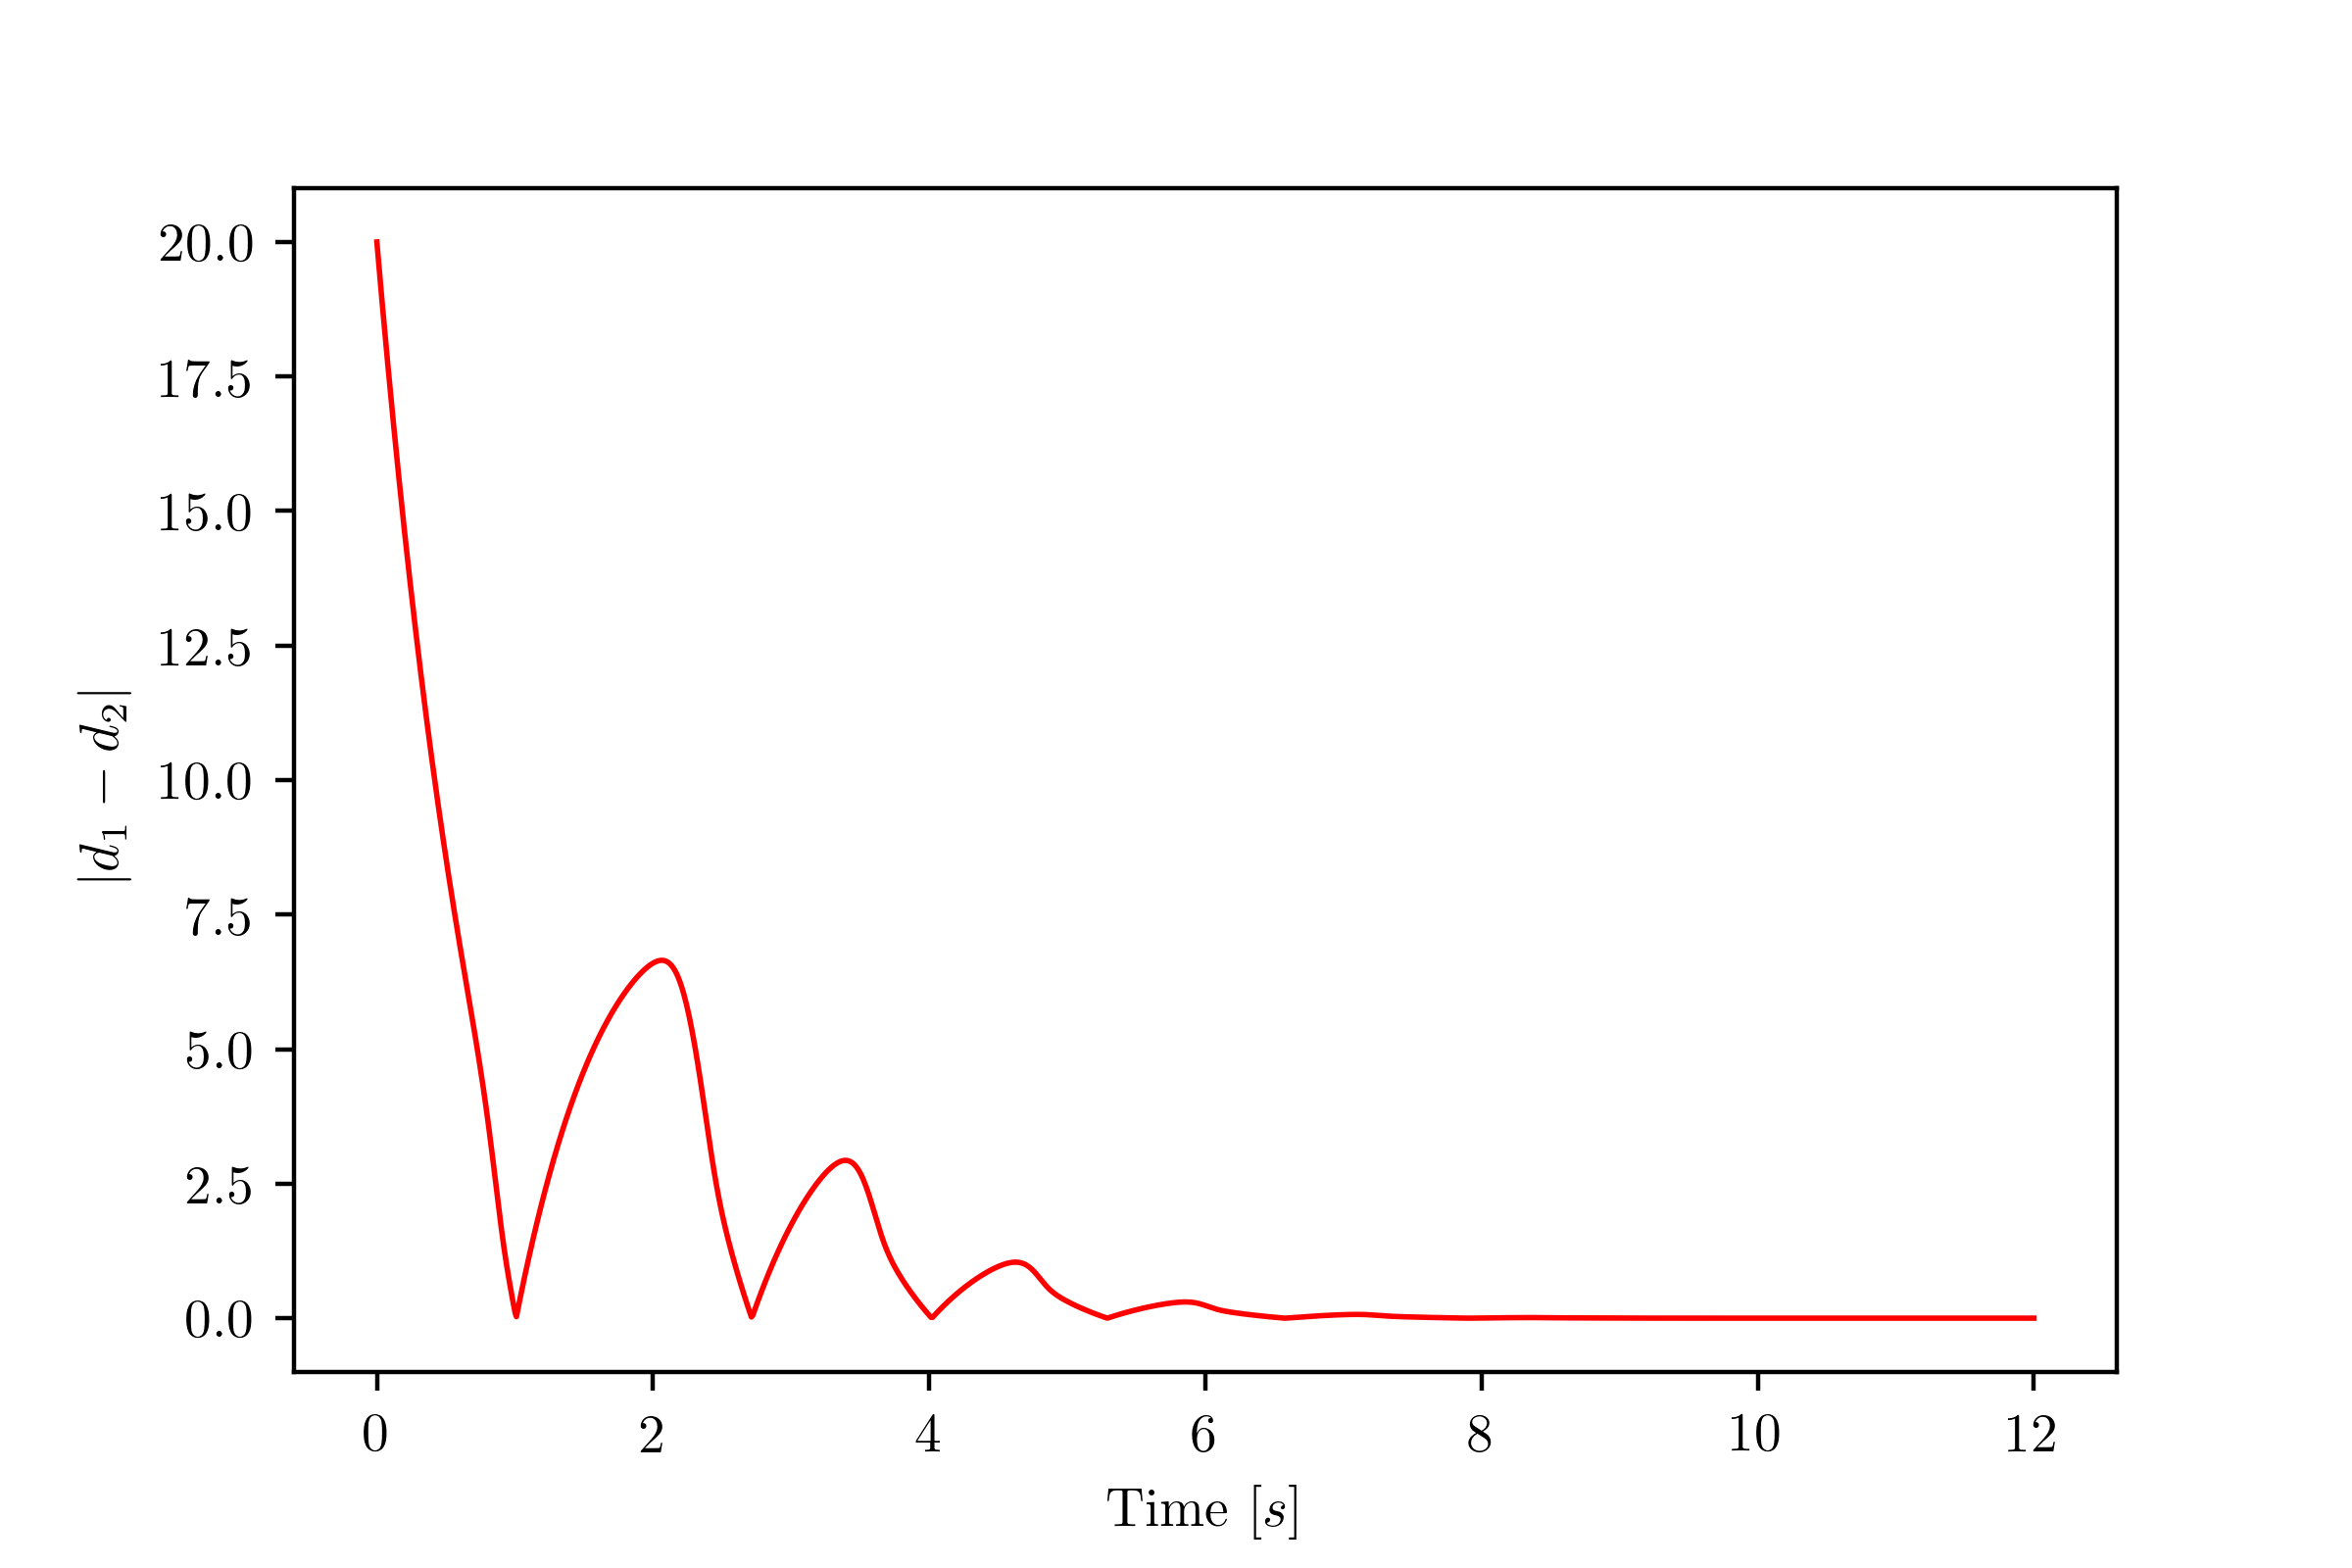
\includegraphics[width=\textwidth]{text/analysis/fig/2by2adapt/synch_2_by_2.png}}
        \caption{\label{fig:2_2_synch} Dynamics of the absolute error $|d_1-d_2|$}
\end{figure}

In order to study the stability of the synchronisation set $M$, one can study the error dynamics $d=d_1 - d_2$ and $e= e_1 - e_2$ and its stability. 

\begin{equation} 
\begin{aligned}
\dot d &= -d - e - \varepsilon \cdot (f(d_1) - f(d_2)) \\
\tau_e \dot e &= g_a \cdot (f(d_1) - f(d_2)) - e
\end{aligned}
\end{equation}


 We would like to replace the quantity $f(d_1) - f(d_2)$ with some function of the only difference of $d=d_1-d_2$. Unfortunately, this is not possible since $f(d_1)-f(d_2) = \frac{e^{d_1}-e^{d_2}}{(1+e^{d_1})(1+e^{d_2})}$. Nevertheless it could be interesting to see $f(d_1)-f(d_2)$ as a time-varying function $g(d, t)$ and analyse some properties that are preserved during the evolution of the system.
It is easy to prove that:
\begin{equation}
\begin{aligned}
|g(d,t)| &\leq \frac{1}{2}d(t) \\
g(d,t)&d>0, \forall t, d\neq0
\end{aligned}
\end{equation}
\textbf{Missing part about Lyapunov stability analysis.}

\paragraph{Bifurcation Analysis}
Once we have proven that the synchronisation manifold (or set) is Globally Asymptotically Stable we can study the dynamics of the system restricted on it. Remember that in $M$ it holds that $d_1=d_2$, therefore we can study the dynamics of the two identical units independently.  
\begin{equation}
\begin{aligned}
\dot d_{1} &= - d_1 - e_1 + \varepsilon f(d_1) \\
\tau_a \dot{e}_{1}&=g_a f(d_1) - e_{1}\\
f(d_1) &= \frac{e^{d_1}-1}{e^{d_1}+1}
\end{aligned}
\label{eq:2D_sync}
\end{equation}

We will start the analysis of this two dimensional system by computing the equilibria $(d_1^*,e_1^*)$ and study their properties with the variation of the parameters $\varepsilon, g_a$. The time constant $\tau_a$ is kept fixed, considered as a typical constant of the system. Notice that the system has a global symmetry property: for each solution $(d_1(t), e_1(t))$ it holds that also $(-d_1(t), -e_1(t))$ is a solution. The roots of the equations below \eqref{eq:eq_d_eq}, \eqref{eq:eq_e_eq}  are the fixed points of the dynamics in \eqref{eq:2D_sync}.
\begin{equation}
 (\varepsilon - g_a)f(d_1^*) - d_1^* = 0
\label{eq:eq_d_eq}
\end{equation}
\begin{equation}
e_1^* = g_a f(d_1^*)
\label{eq:eq_e_eq}
\end{equation}

The number of equilibria is uniquely defined by the quantity $\varepsilon-g_a$. In particular, it is easy to show analitically that there is a unique equilibrium for $\varepsilon \leq g_a-2$, while for $\varepsilon > g_a-2$ we have three equilibrium points. Unfortunately, since the equilibria can not be computed analytically we will make use of numerical analysis. In \cref{fig:eq2D_adapt} the three most important cases are plotted.

 \begin{figure}[!h]
        \center{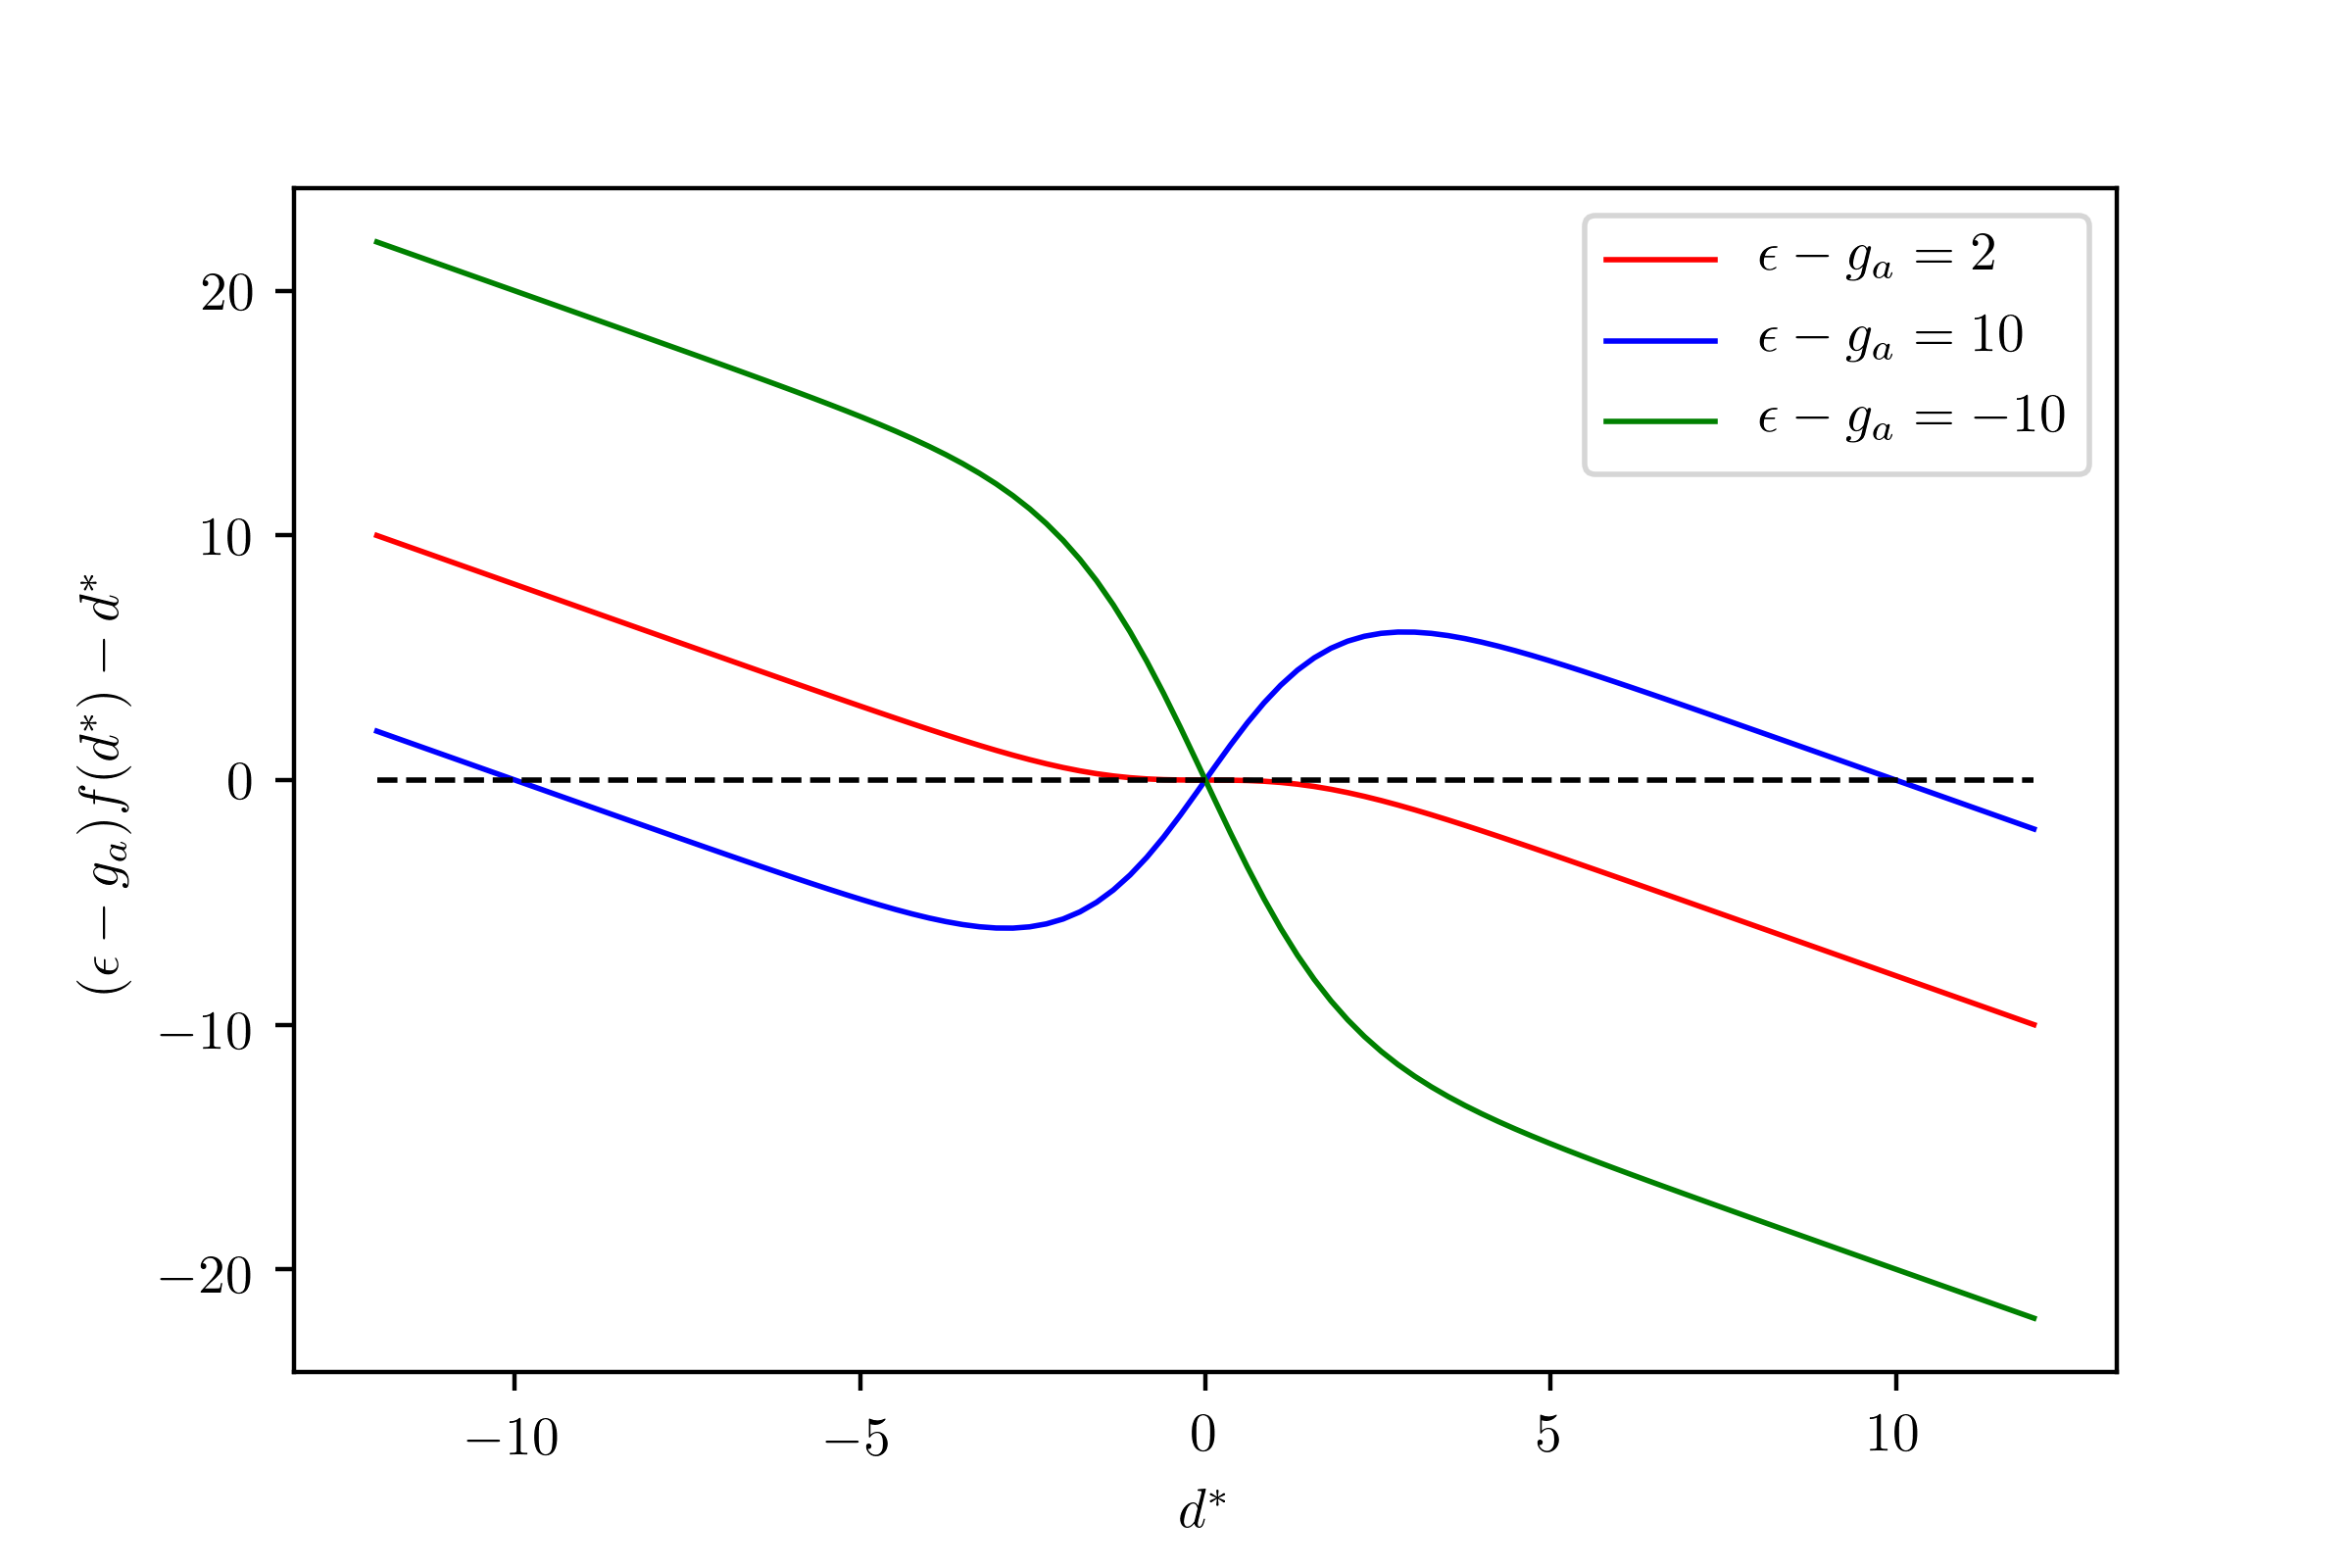
\includegraphics[width=\textwidth]{text/analysis/fig/2by2adapt/equilibria_2D.png}}
        \caption{\label{fig:eq2D_adapt} Graphical visualization of the roots of the equation in \eqref{eq:eq_d_eq}} with varying the quantity $\varepsilon - g_a$.
\end{figure}

We will first analyse the system with $\varepsilon - g_a < 2$. With this choice of parameters the unique equilibrium is the point $(d_1^*,e_1^*)=(0, 0)$. The computed jacobian matrix $J_{(0,0)}$ and the characteristic polynomial are the following:

\begin{equation}
J_{(0, 0)} = \begin{bmatrix} 
\frac{\varepsilon}{2} & -1 \\
\frac{g_a}{2\tau_a} & -\frac{1}{\tau}
\end{bmatrix}
\end{equation}

\begin{equation}
\rho(\lambda) = \lambda^2 +  \frac{2\tau_a + 2 - \tau_a \varepsilon}{2\tau_a} \lambda + \frac{-2\varepsilon + 2g_a + 4}{4\tau_a}
\end{equation}

\begin{equation}
\rho(\lambda) = \lambda^2 + a\lambda +b
\end{equation}

In order to study the stability of the equilibrium point one can study the sign of the polynomial's coefficient. In fact for a second order polynomial, the number of roots with positive real part can be determined by the number of variations in the polynomial's coefficients \cite{gantmacher2005matrix}.

\begin{equation}
\begin{aligned}
 a < 0 \iff & \varepsilon > 2(1 + \frac{1}{\tau_a}) \\
 b < 0 \iff & \varepsilon > g_a + 2
\end{aligned}
\end{equation}

When $\varepsilon<2(1+\frac{1}{\tau_a})$ the origin is an asymptotically stable equilibrium point. This condition is not particularly interesting since it means that all the units in the network converge to the same value and their output is identical. In other words, the network is not able to recall any pattern (\cref{fig:eq2D_focus}).

\begin{figure}[!h]
        \center{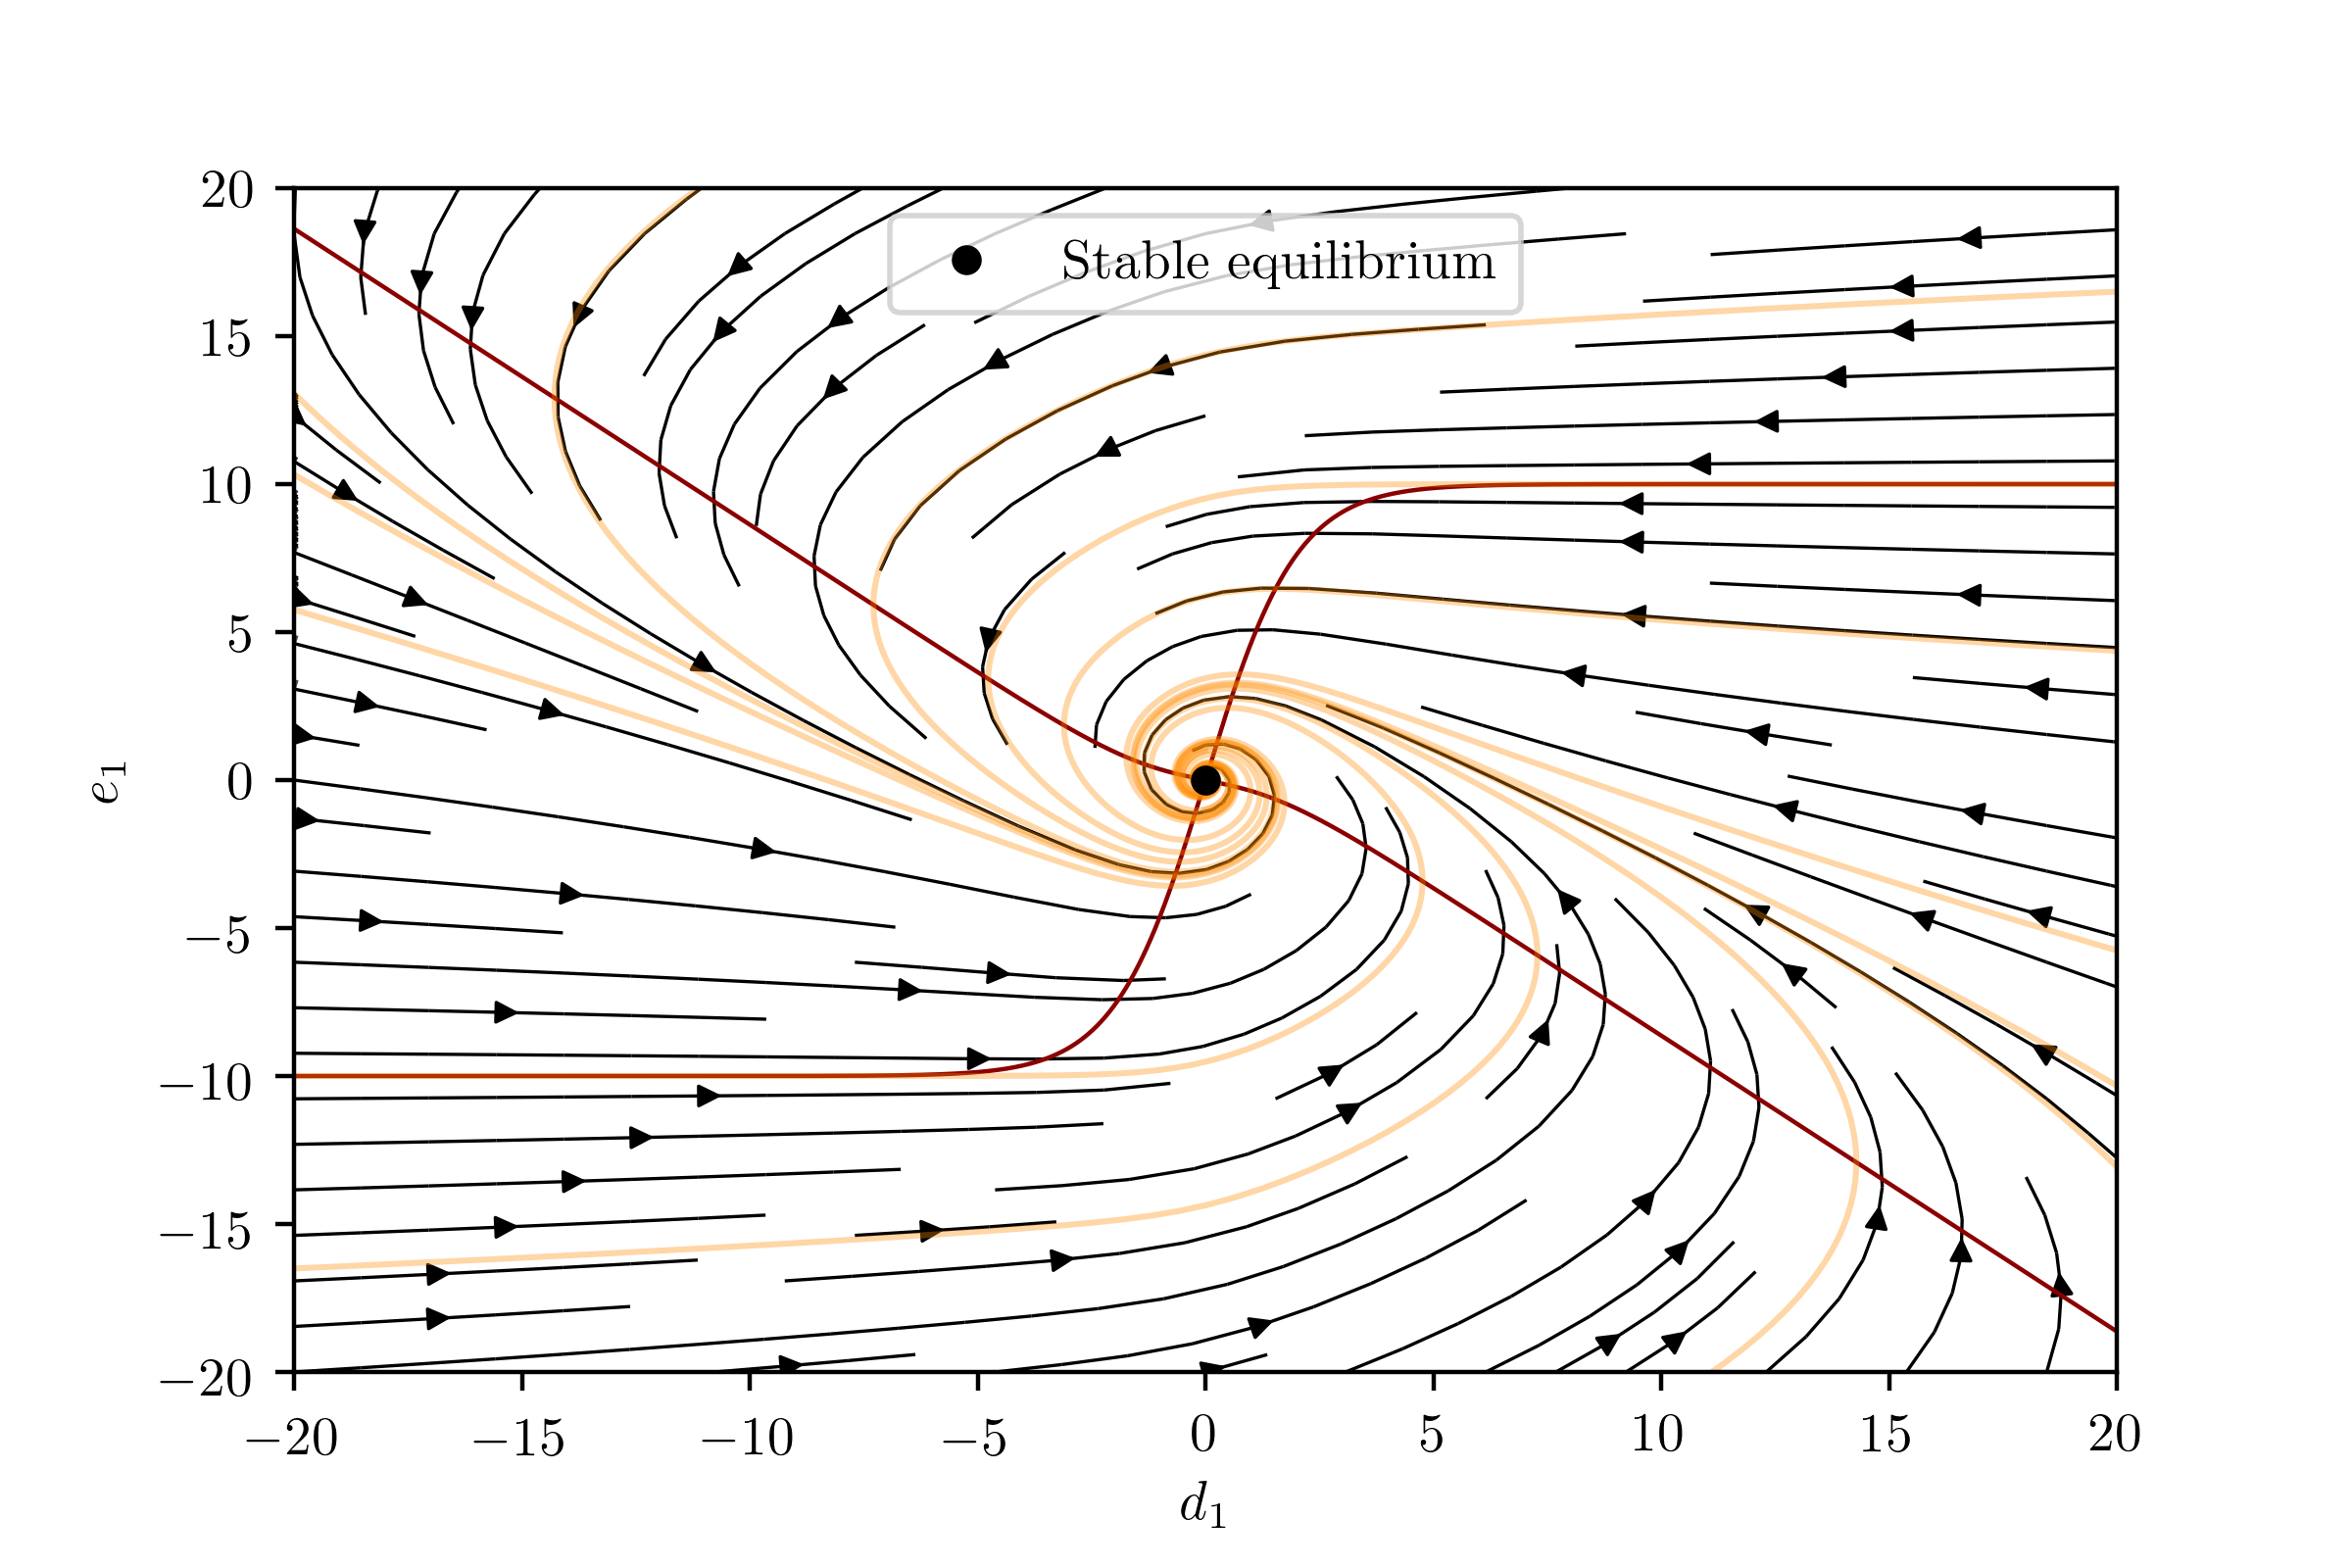
\includegraphics[width=\textwidth]{text/analysis/fig/2by2adapt/streamline_stable_focus.png}}
        \caption{\label{fig:eq2D_focus} Phase portrait of system in \eqref{eq:2D_sync} for $\varepsilon=1.5,\ g_a=10,\ \tau_a=2$. The nullclines are shown in dark red; the streamline plot is shown in black; several trajectories of the system with different initial conditions are shown in orange.}
\end{figure}


At the critical value $\varepsilon^* = 2 ( 1 + \frac{1}{\tau_a} ) $ a \textbf{supercritical Hopf} bifurcation occurs. In fact, as $\varepsilon$ passes through $\varepsilon^*$, the complex eigenvalues $\lambda_{1,2}$ crosses the imaginary axis. In fact, ${\rm I\!R}(\lambda_{1,2})<0, \varepsilon < \varepsilon^*$ and  ${\rm I\!R}(\lambda_{1,2})>0, \varepsilon > \varepsilon^*$. Therefore, the equilibrium point $(0, 0)$ changes its stability and a unique stable limit cycle bifurcates from it (\cref{fig:eq2D_cycle}).
\begin{figure}[!h]
        \center{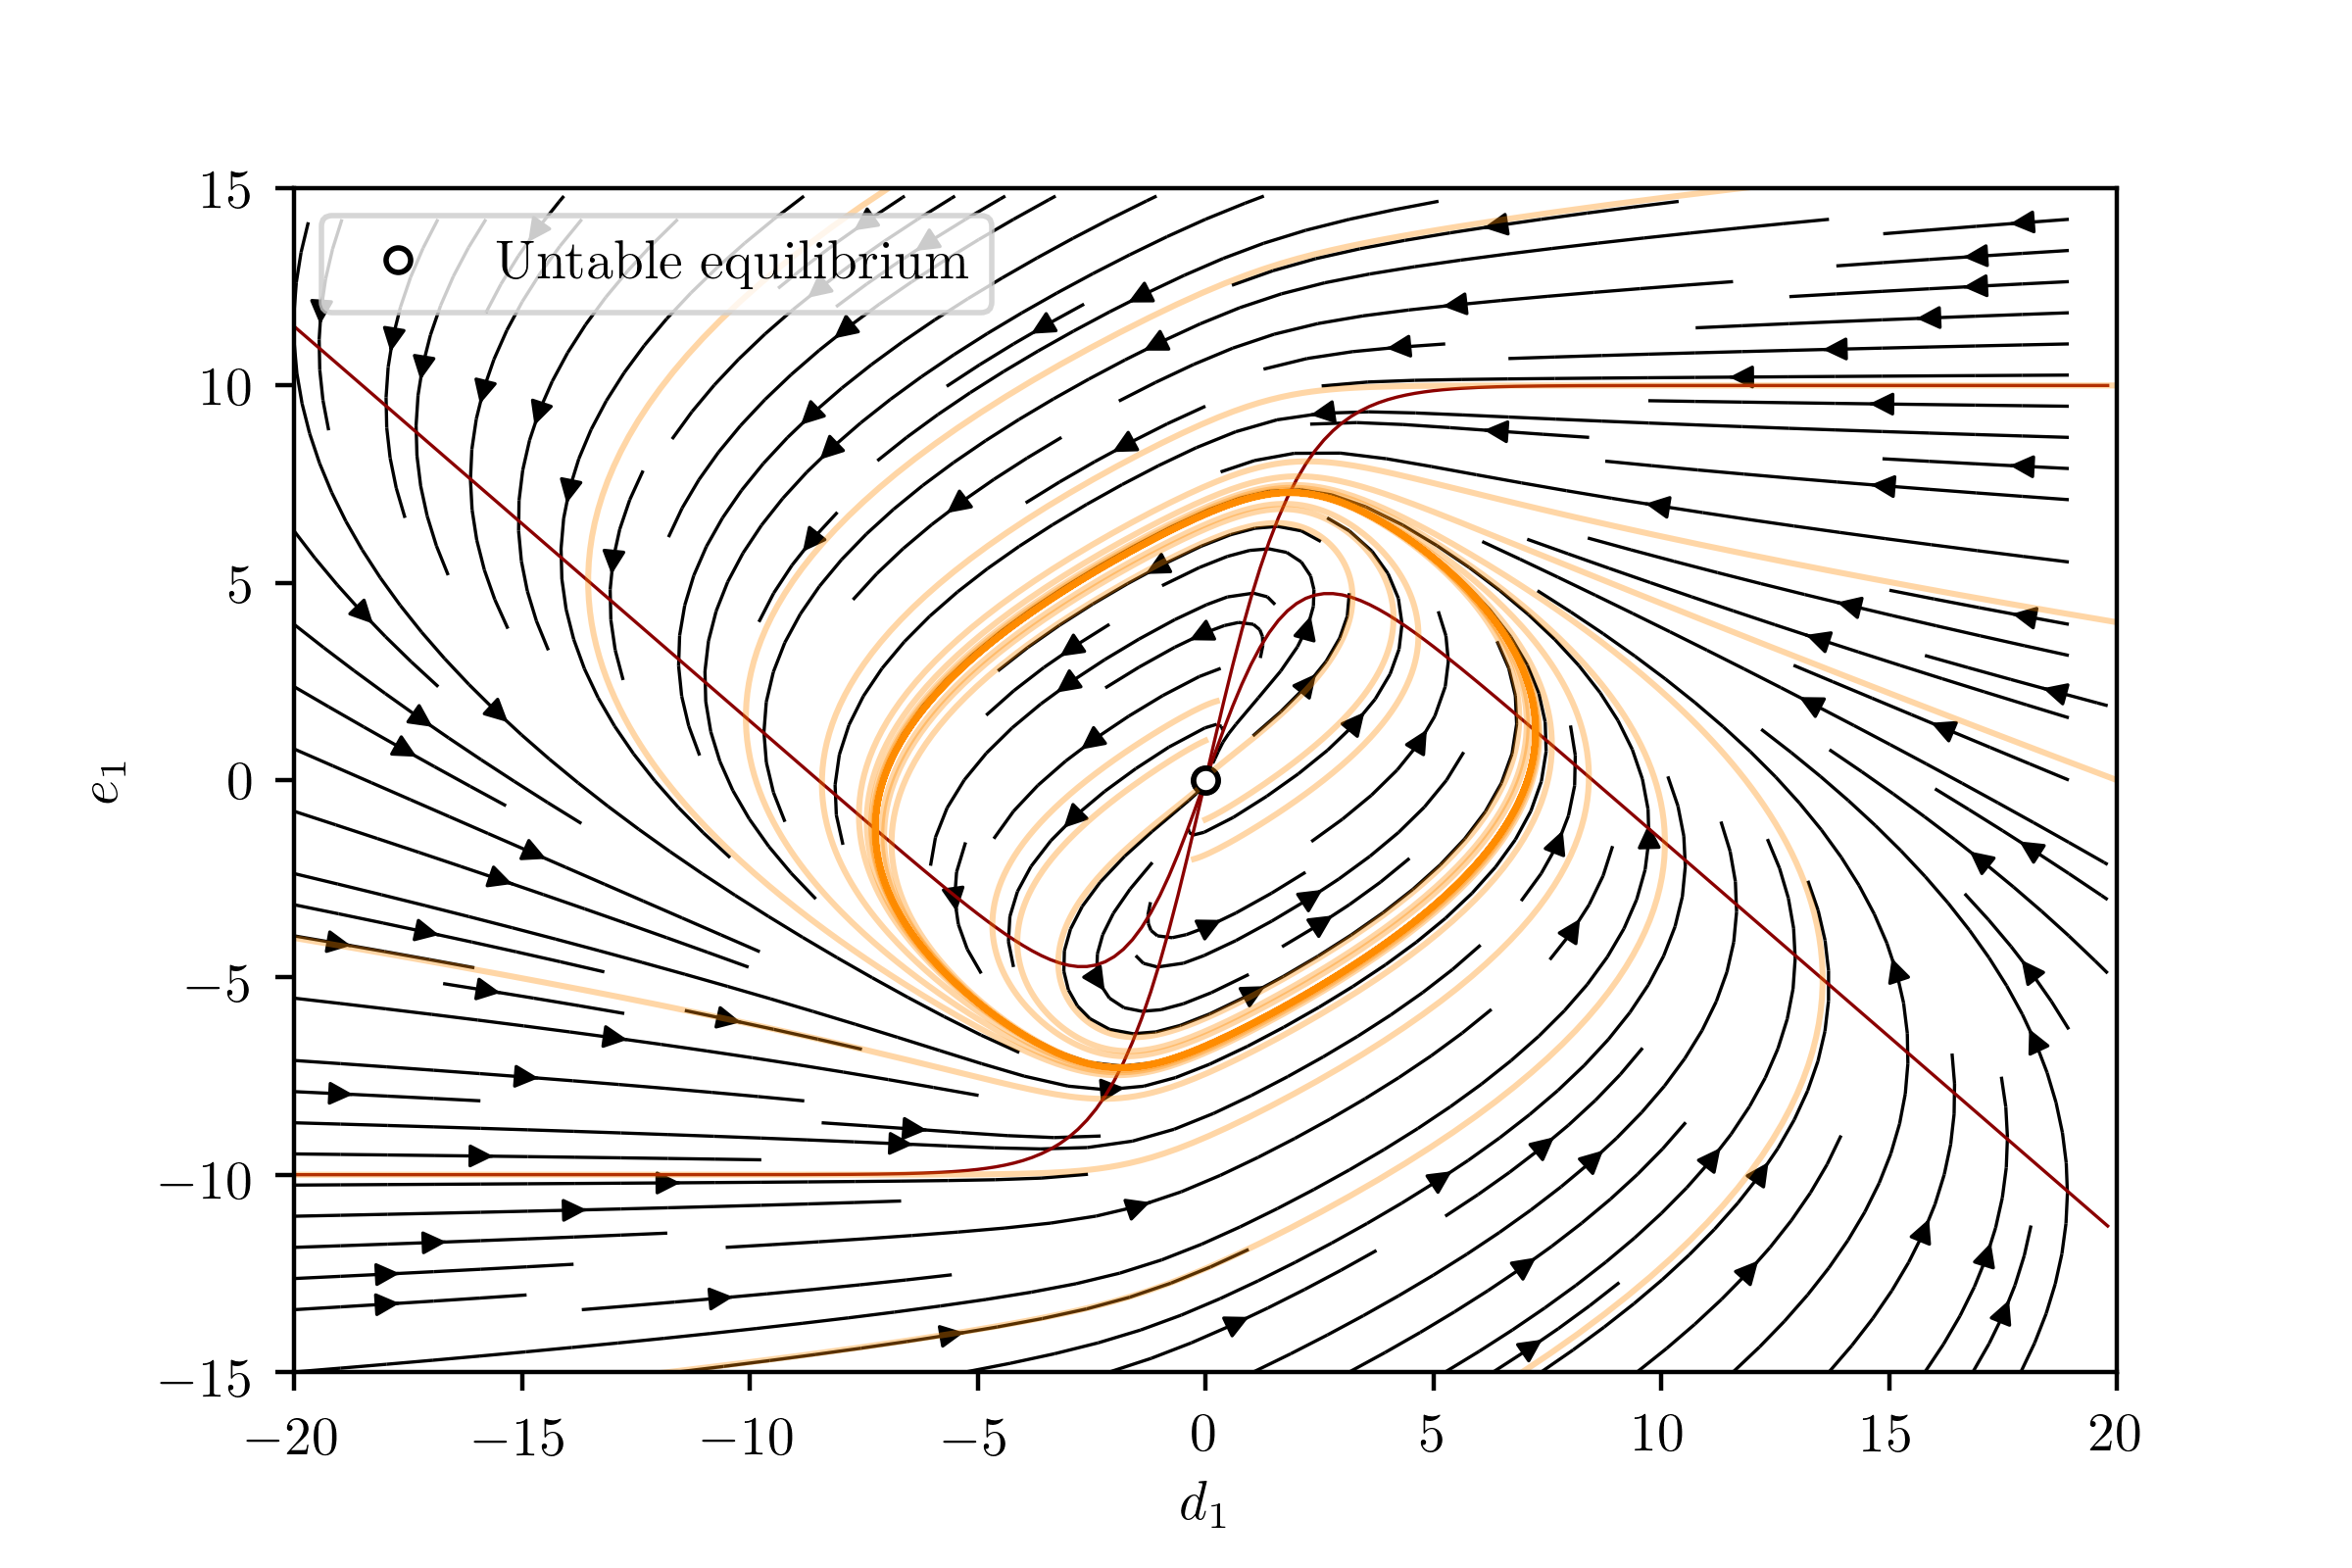
\includegraphics[width=\textwidth]{text/analysis/fig/2by2adapt/streamline_cycle.png}}
        \caption{\label{fig:eq2D_cycle} Phase portrait of system in \eqref{eq:2D_sync} for $\varepsilon=8.5,\ g_a=10,\ \tau_a=2$. The nullclines are shown in dark red; the streamline plot is shown in black; several trajectories of the system with different initial conditions are shown in orange.}
\end{figure}


But what happens when the coupling factor $\varepsilon$ increases? The next interesting bifurcation phenomenon occurs at the critical value $\varepsilon^o = g_a + 2$ when a \textbf{supercritical pitchfork bifurcation} occurs. In fact, the origin spawns two unstable equilibria and \textit{changes from unstable node to saddle node. What counts for bifurcations is what happens on the center manifold}. While the parameter $\epsilon > \epsilon^o$ keeps increasing the additional two equilibria moves far away from the origin and additional bifurcations occur. In particular, one can numerically find that at ... hopf bifurcation happens again.


\begin{figure}[!h]
        \center{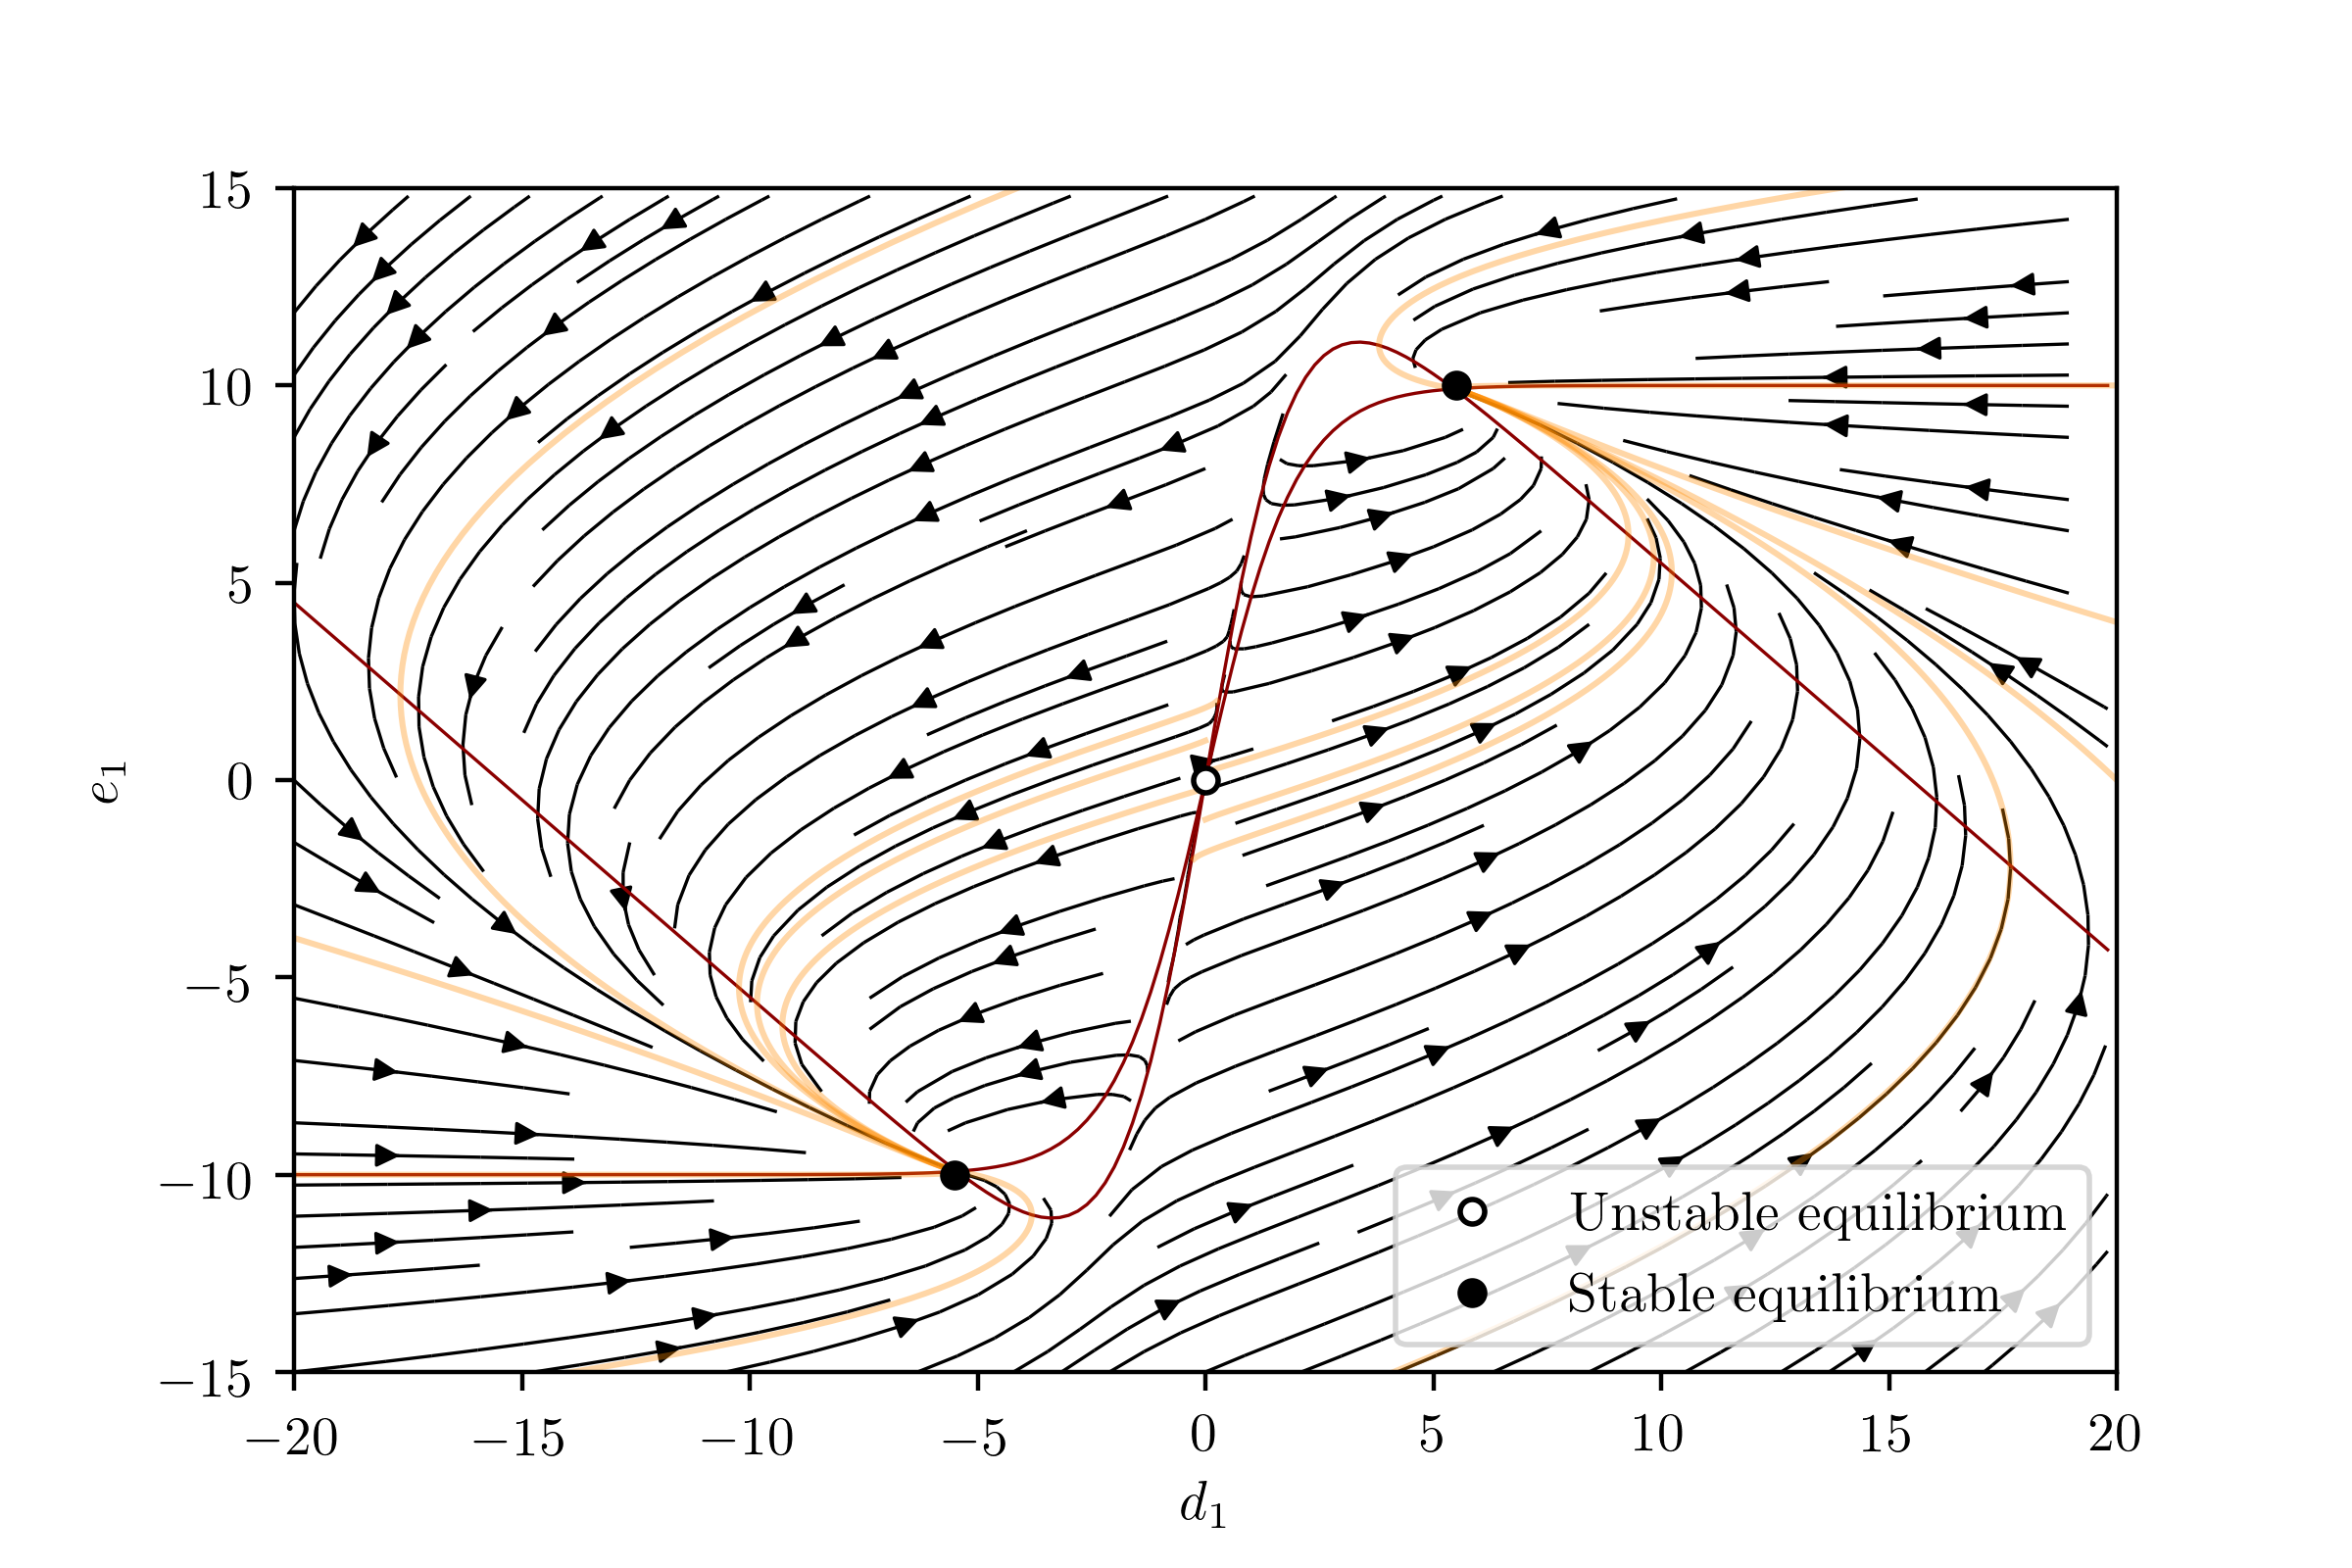
\includegraphics[width=\textwidth]{text/analysis/fig/2by2adapt/streamline_fixed.png}}
        \caption{\label{fig:eq2D_mem}Two equilibria}
\end{figure}
Consider a complete, homogeneous graph of $N$ hypercolumns, each one consisting of 2 minicolumns. Denote $w$ the weight, identical for all the edges, it follows that $\alpha=(N-1)w$. Therefore, on the synchronization manifold, we can describe the dynamics of the single oscillators independently.
\begin{equation}
\begin{aligned}
    \tau_m \dot{s}_{11}&=-s_{11}-a_{11}+ \alpha o_{11} \\
    \tau_a \dot{a}_{11}&=g_a o_{11} - a_{11} \\
    \tau_m \dot{s}_{12}&=-s_{12}-a_{12}+ \alpha o_{12} \\
    \tau_a \dot{a}_{12}&=g_a o_{12} - a_{12} \\
\end{aligned}
\label{eq:complete_dynamics}
\end{equation}

The system described in \eqref{eq:complete_dynamics} is a 4 dimensional system but its analysis can be easily simplified by exploiting some nice properties of the output softmax function. In particular the two following properties hold:  
\begin{equation}
 \sum_{k=1}^{m} o_{i k}=1
 \label{soft_sum}
\end{equation}
\begin{equation}
 f(d_i)= o_{i1}-o_{i2}=\frac{e^{d_i}-1}{e^{d_i}+1}, \quad d_i = s_{i1}-s_{i2}
 \label{soft_diff}
\end{equation}
Given \eqref{soft_sum} and \eqref{soft_diff} we can introduce the following change of variables that will help us to significantly simplify the analysis of the dynamics and also get a deeper insight into the behaviour of our system. 
\begin{equation}
\begin{aligned}
z_1 &= s_{11} + s_{12} \\
w_1 &= a_{11} + a_{12} \\
d_1 &= s_{11} - s_{12} \\
e_1 &= a_{11} - a_{12} \\
\end{aligned}
\end{equation}
The dynamics in the new coordinate follows:
\begin{equation} 
\begin{aligned}
\tau_m \dot z_1 &= - z_1 - w_1 + \alpha\\
\tau_a \dot w_1 &= g_a - w_1
\end{aligned}
\label{eq:sum_dynamics}
\end{equation}
\begin{equation} 
\begin{aligned}
\tau_m \dot d_{1} &= - d_1 - e_1 + \alpha f(d_1) \\
\tau_a \dot{e}_{1} &= g_a f(d_1) - e_{1} \\
\end{aligned}
\label{eq:diff_dynamics}
\end{equation}

The dynamics of coupled variables $(z_1, w_1)$ is linear and it trivially holds that the equilibrium point $(z_1^*,w_1^*)=(-g_a+\alpha, g_a)$ is globally asymptotically stable. Furthermore, it is interesting to notice that the variables  $(z_1, w_1)$ are completely decoupled from $(d_1, e_1)$ since they do not appear in the former's dynamics. The nonlinear dynamics for $d, e$ is much richer and requires further analysis. 

\paragraph{Bifurcation Analysis}
We start the analysis of the two dimensional system in \cref{eq:diff_dynamics} by computing the equilibria $(d_1^*,e_1^*)$ and study their stability properties with the variation of the parameters $\alpha, g_a$. As discussed in \cite{LansnerFRC} the adaptation dynamics is much slower than the support dynamics, i.e. $\tau_a > \tau_m$. Keeping in mind that what defines the dynamics is the ratio $\tau_a/\tau_m$, for the rest of the analysis we will keep $\tau_a>1$ fixed, considered as a typical constant of the system and $\tau_m=1$. Notice that the system has a global symmetry property: for each solution $(d_1(t), e_1(t))$ it holds that also $(-d_1(t), -e_1(t))$ is a solution. The roots of the equations below \eqref{eq:eq_d_eq}, \eqref{eq:eq_e_eq} are the equilibria of the dynamics in \eqref{eq:diff_dynamics}.
\begin{equation}
 (\alpha - g_a)f(d_1^*) - d_1^* = 0
\label{eq:eq_d_eq}
\end{equation}
\begin{equation}
e_1^* = g_a f(d_1^*)
\label{eq:eq_e_eq}
\end{equation}

The number of equilibria is uniquely defined by the quantity $\alpha-g_a$. In particular, it is easy to show that there is a unique equilibrium for $\alpha \leq g_a-2$, while for $\alpha > g_a-2$ we have three equilibrium points. Unfortunately, since the equilibria can not be computed analytically we will make use of numerical analysis. In \cref{fig:eq2D_adapt} the three most important cases are plotted.

 \begin{figure}[!h]
        \center{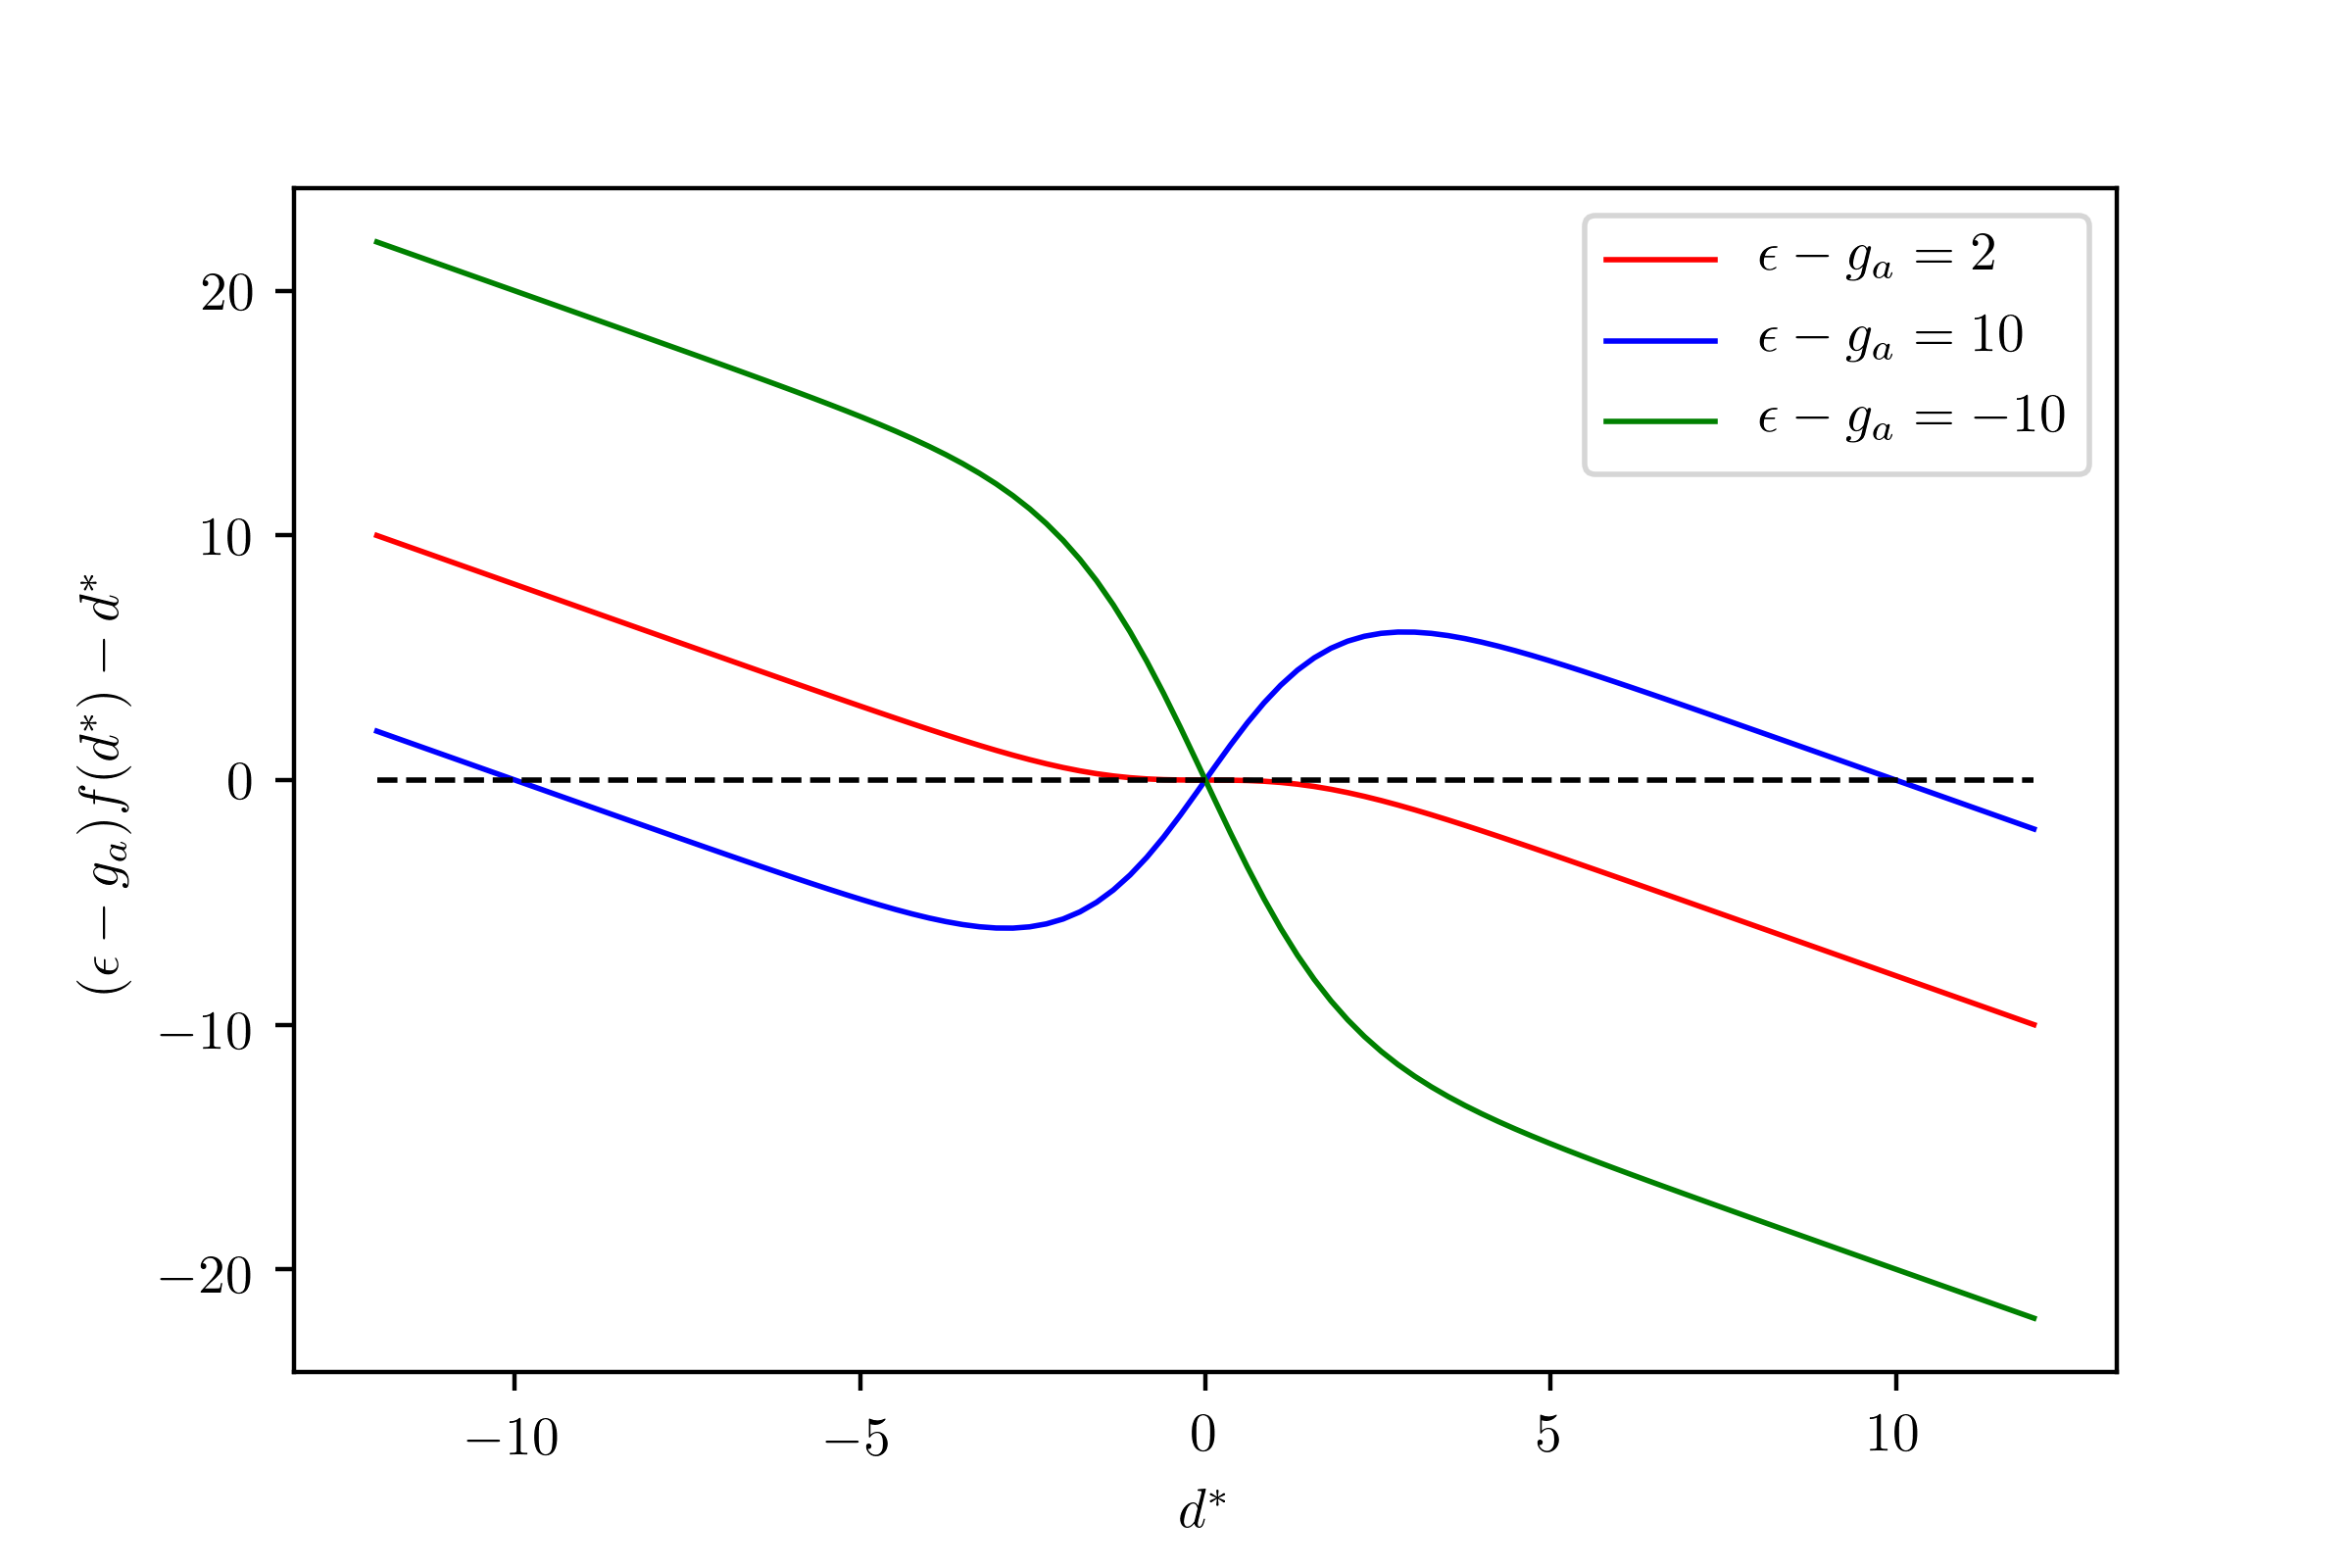
\includegraphics[width=\textwidth]{text/analysis/fig/2by2adapt/equilibria_2D.png}}
        \caption{\label{fig:eq2D_adapt} Graphical visualization of the roots of the equation in \eqref{eq:eq_d_eq}} with varying the quantity $\alpha - g_a$.
\end{figure}

We will first analyse the system with $\alpha - g_a < 2$. With this choice of parameters the unique equilibrium is the point $(d_1^*,e_1^*)=(0, 0)$. The computed jacobian matrix $J_{(0,0)}$ and the characteristic polynomial are the following:

\begin{equation}
J_{(0, 0)} = \begin{bmatrix} 
-1 + \frac{\alpha}{2} & -1 \\
\frac{g_a}{2\tau_a} & -\frac{1}{\tau}
\end{bmatrix}
\end{equation}

\begin{equation}
\rho(\lambda) = \lambda^2 +  \frac{2\tau_a + 2 - \tau_a \alpha}{2\tau_a} \lambda + \frac{-2\alpha + 2g_a + 4}{4\tau_a}
\end{equation}

\begin{equation}
\rho(\lambda) = \lambda^2 + a\lambda +b
\end{equation}

In order to study the stability of the equilibrium point one can study the sign of the polynomial's coefficient. In fact for a second order polynomial, the number of roots with positive real part can be determined by the number of variations in the polynomial's coefficients.

\begin{equation}
\begin{aligned}
 a < 0 \iff & \alpha > 2\left(1 + \frac{1}{\tau_a}\right) \\
 b < 0 \iff & \alpha > g_a + 2
\end{aligned}
\end{equation}

When $\alpha<2(1+\frac{1}{\tau_a})$ the origin is an asymptotically stable equilibrium point. This condition is not particularly interesting since it means that all the units in the network converge to the same value and their output is identical. In other words, the network is not able to recall any pattern (\cref{fig:eq2D_focus}).

\begin{figure}[H]
        \center{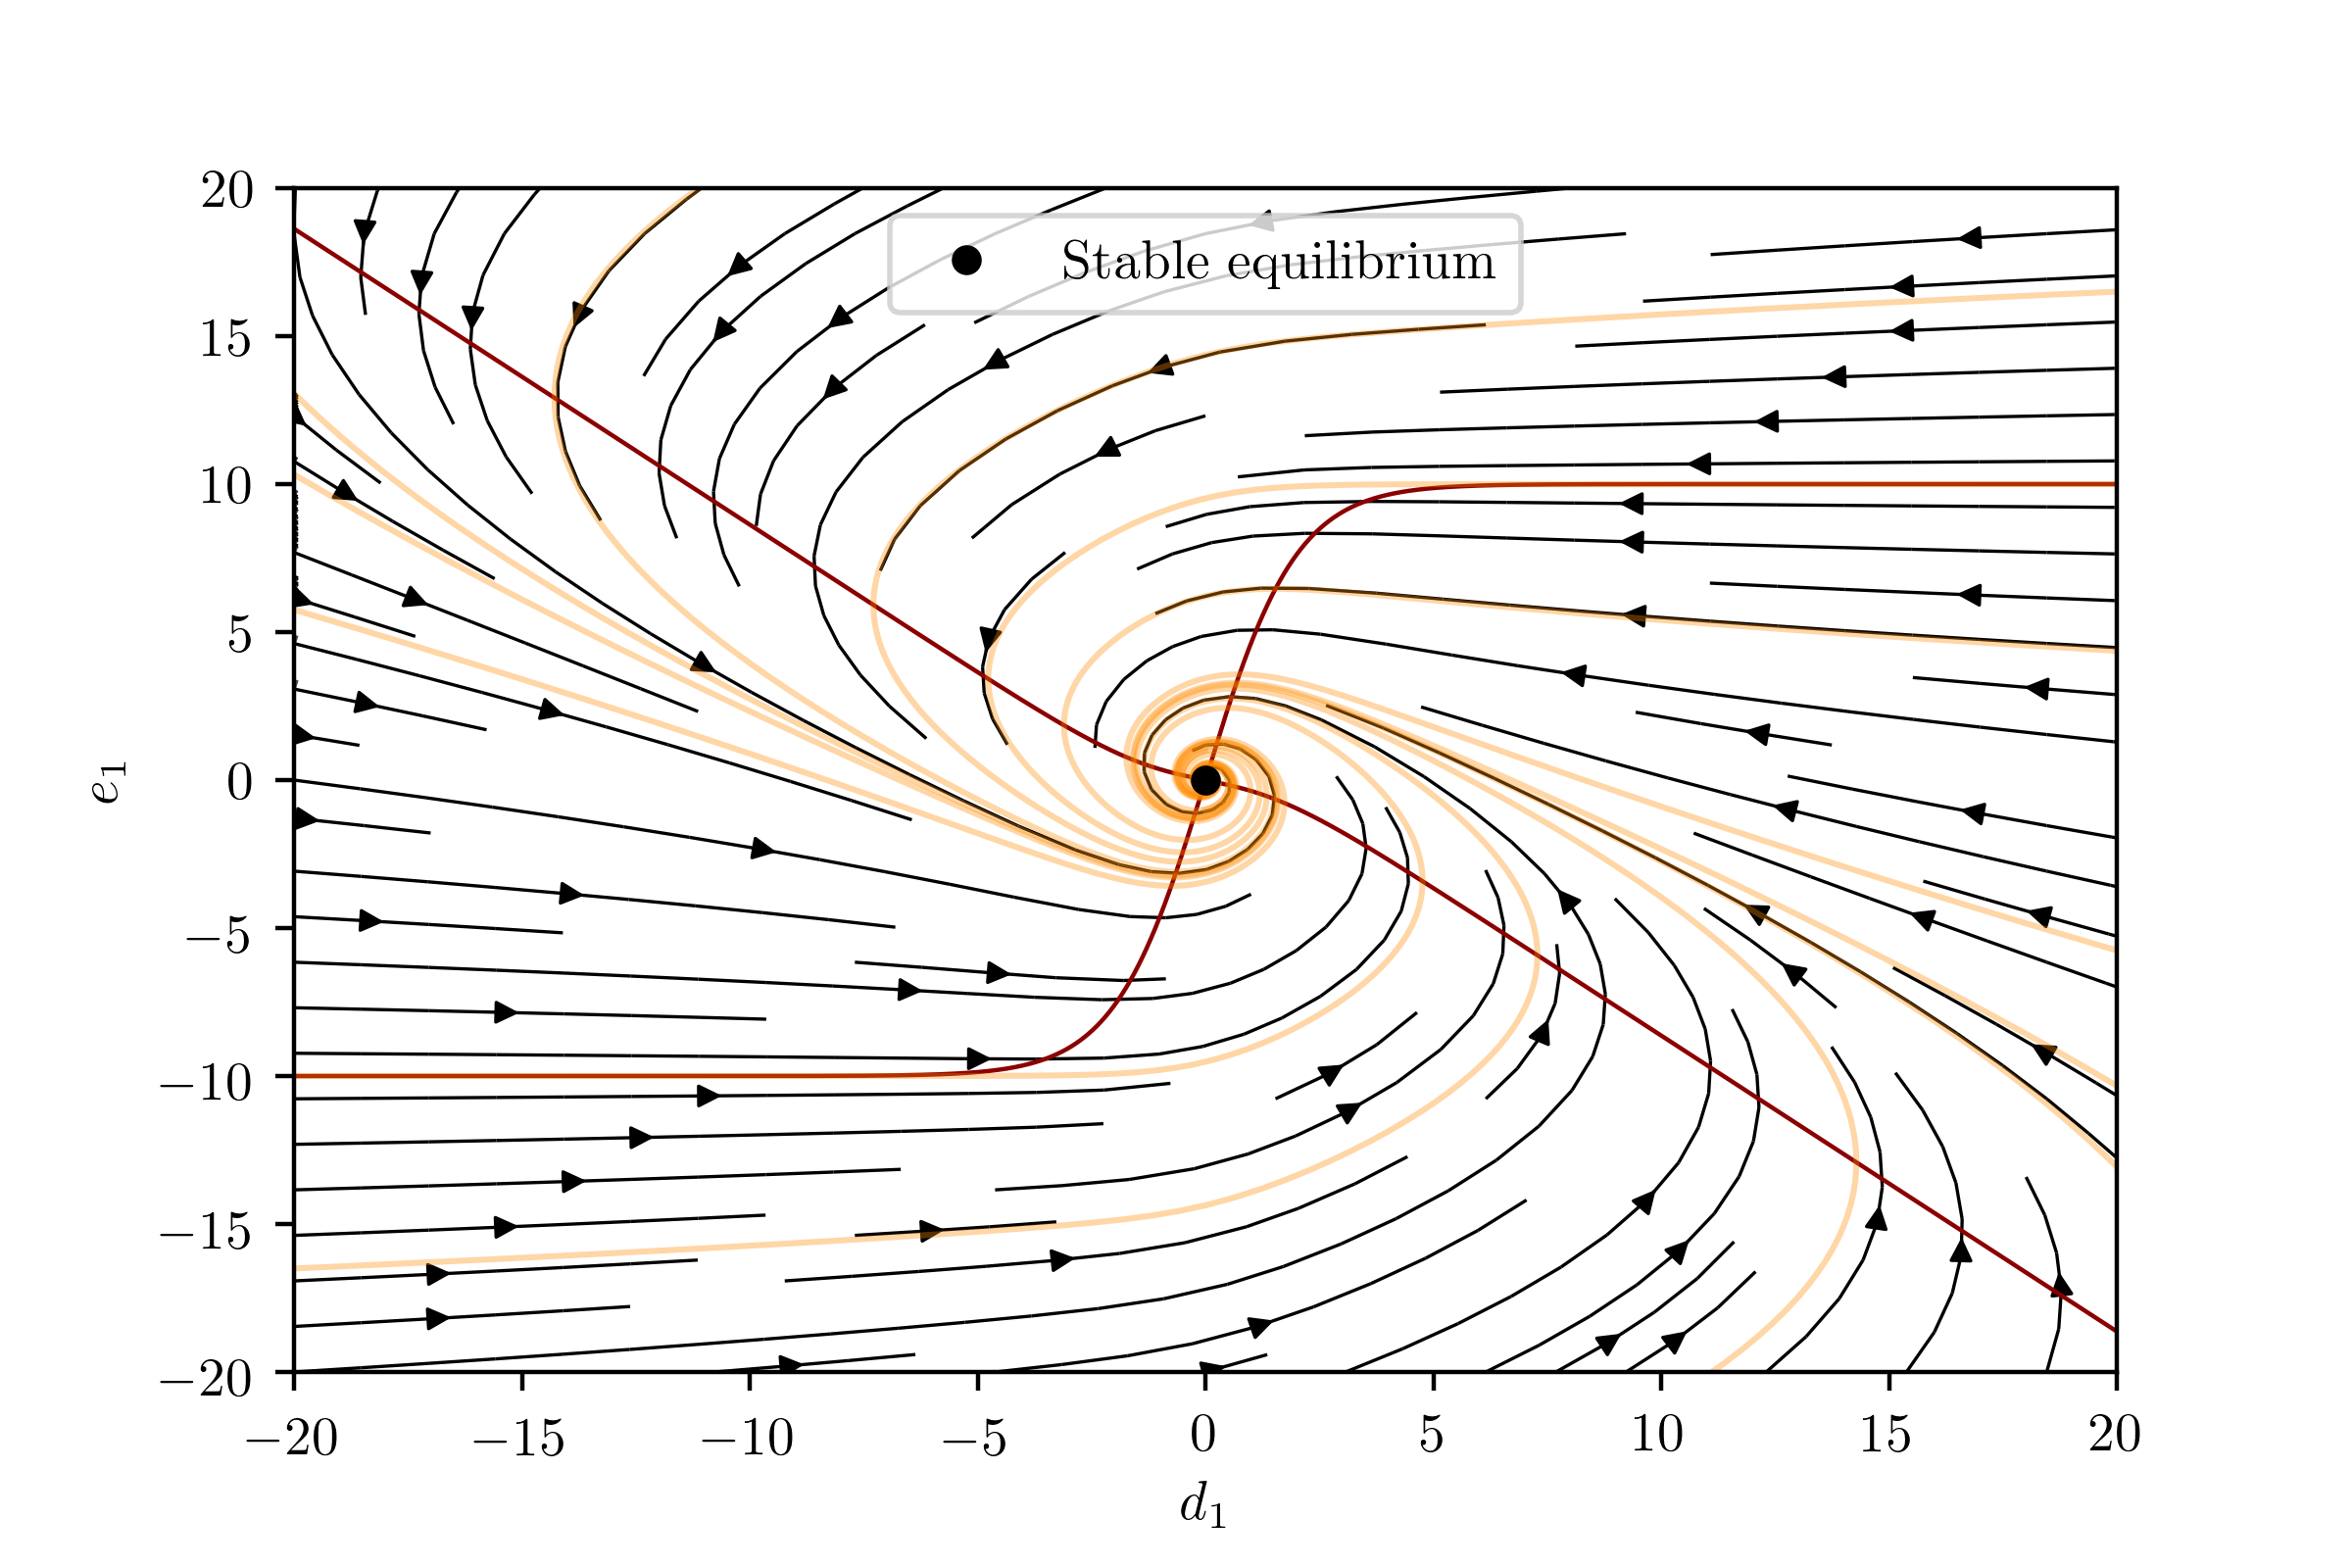
\includegraphics[width=\textwidth]{text/analysis/fig/2by2adapt/streamline_stable_focus.png}}
        \caption{\label{fig:eq2D_focus} Phase portrait of system in \eqref{eq:diff_dynamics} for $\alpha=1.5,\ g_a=10,\ \tau_a=2$. The nullclines are shown in dark red; the streamline plot is shown in black; several trajectories of the system with different initial conditions are shown in orange.}
\end{figure}


At the critical value $\alpha^* = 2 ( 1 + \frac{1}{\tau_a} ) $ a \textbf{supercritical Hopf} bifurcation occurs. In fact, as $\alpha$ passes through $\alpha^*$, the complex eigenvalues $\lambda_{1,2}$ cross the imaginary axis. In fact, ${\rm I\!R}(\lambda_{1,2})<0, \alpha < \alpha^*$ and  ${\rm I\!R}(\lambda_{1,2})>0, \alpha > \alpha^*$. Therefore, the equilibrium point $(0, 0)$ changes its stability and a unique stable limit cycle bifurcates from it (\cref{fig:eq2D_cycle}).

\begin{figure}[H]
        \center{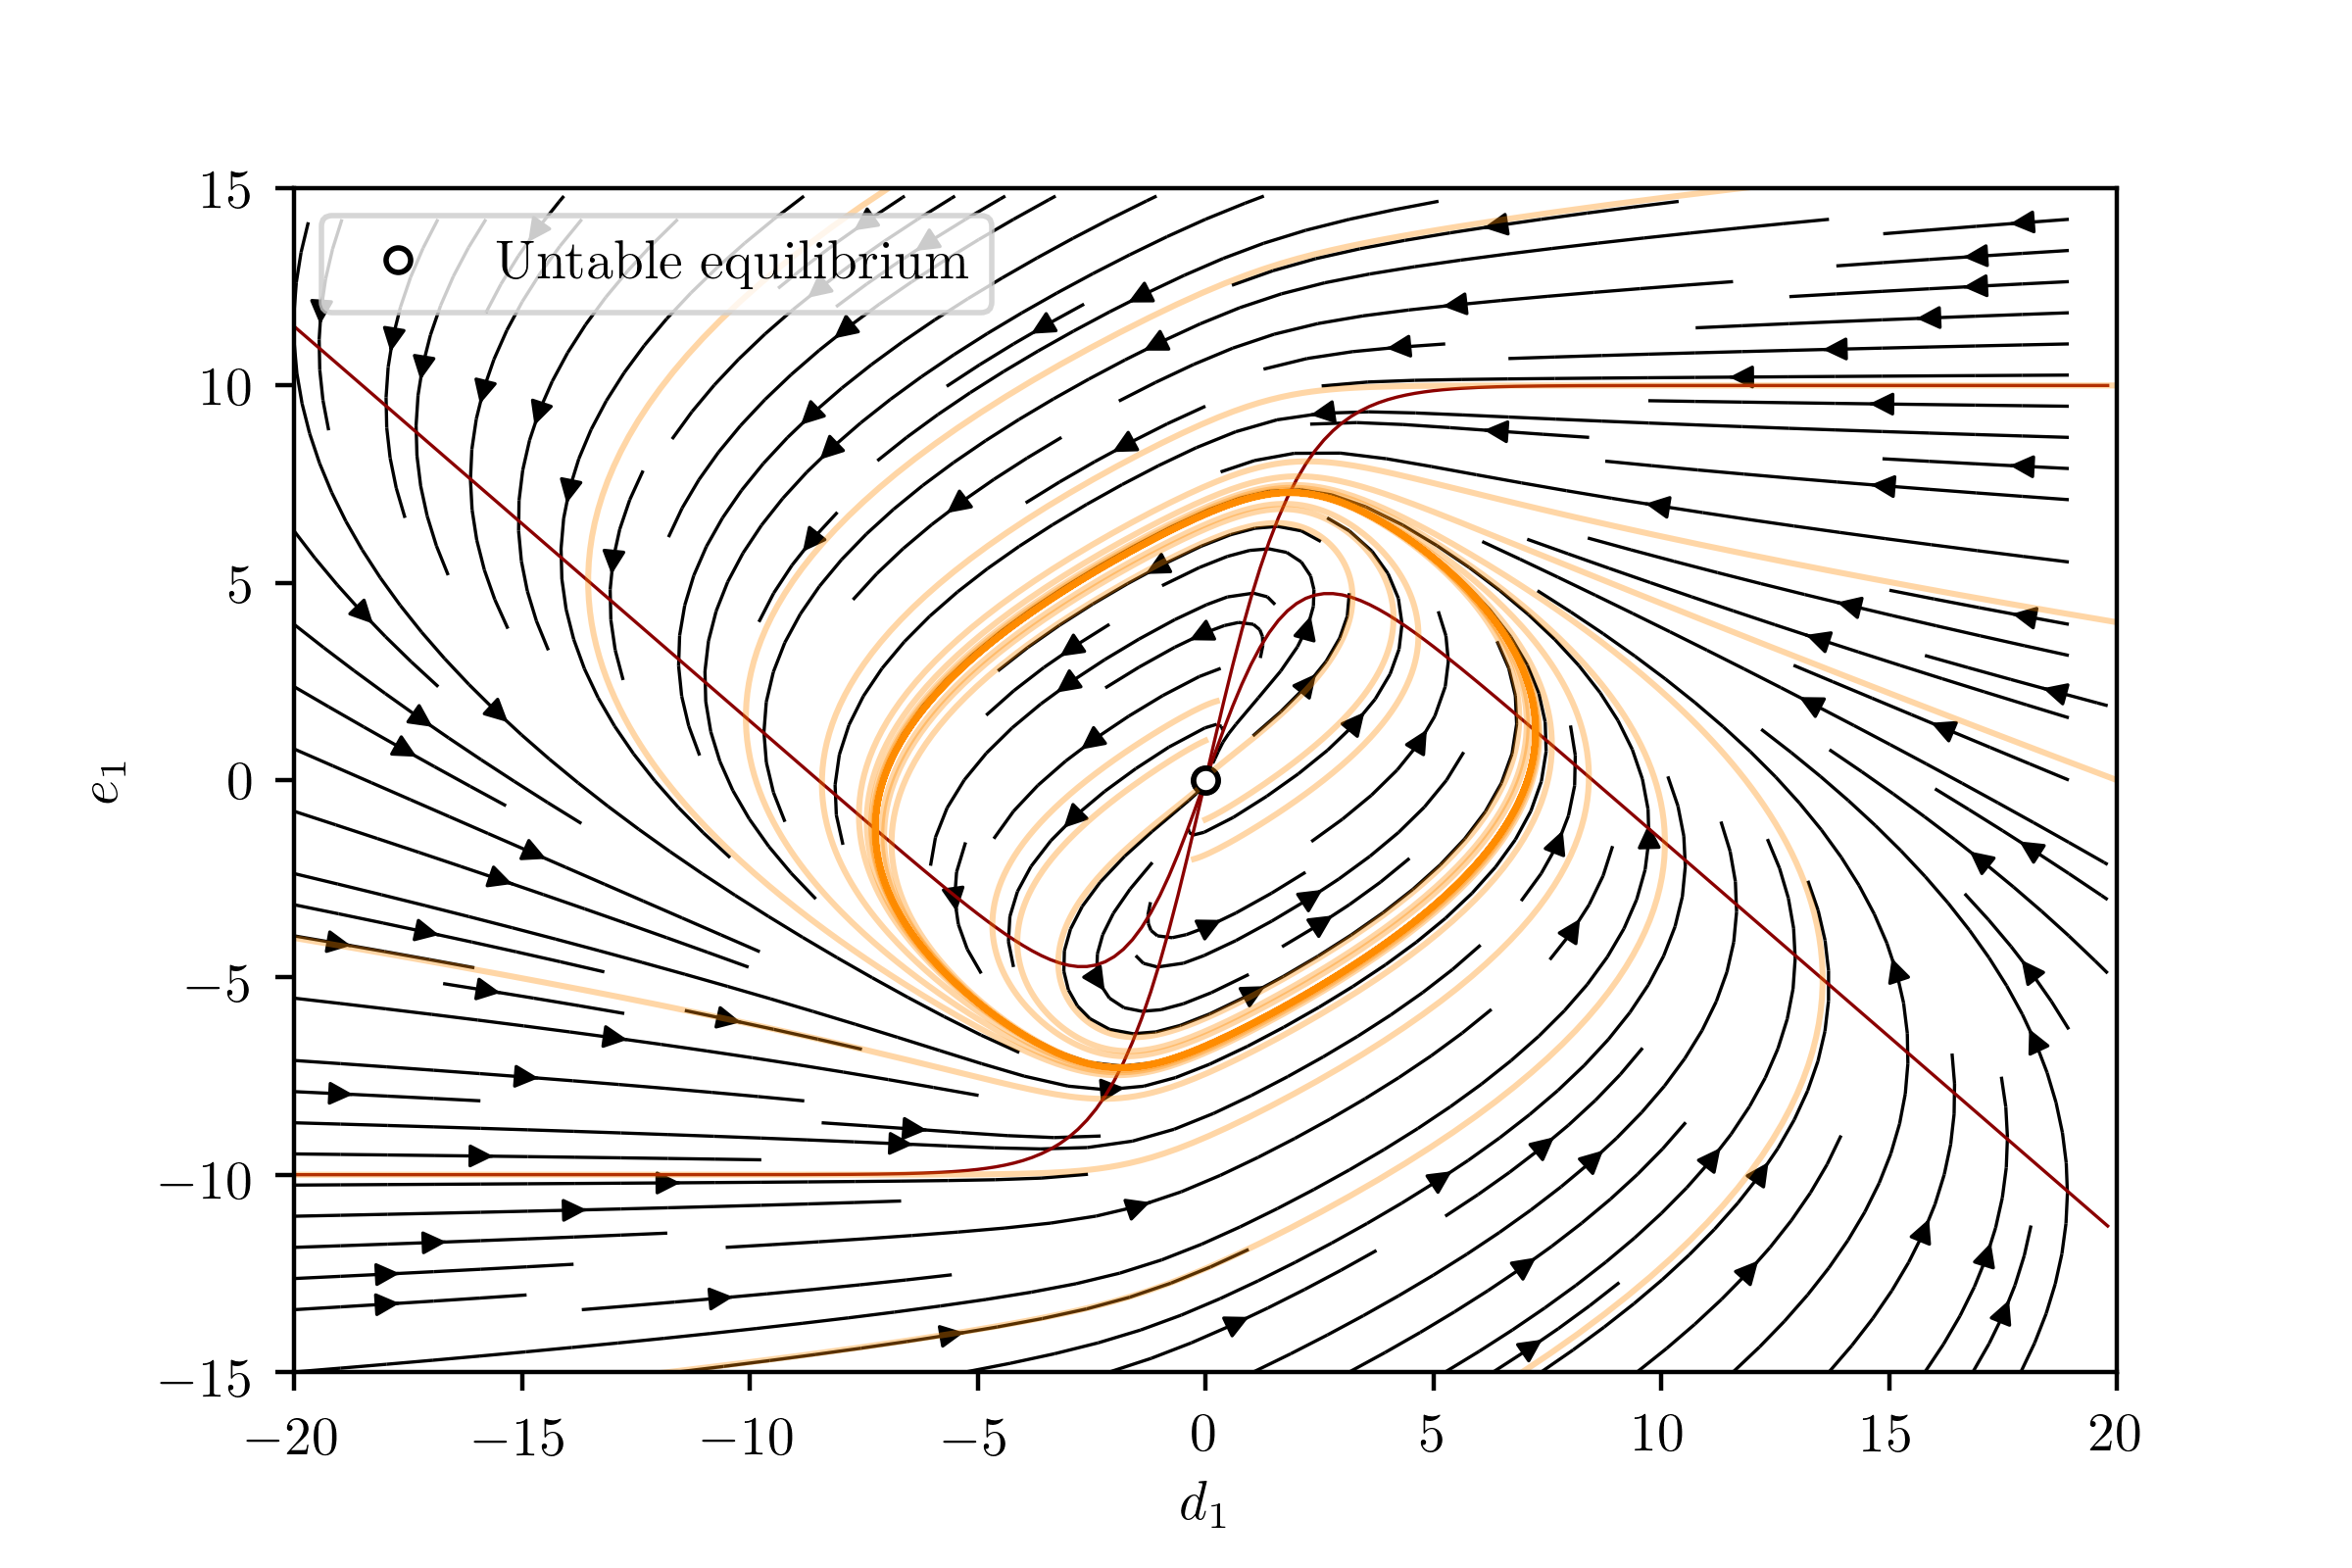
\includegraphics[width=\textwidth]{text/analysis/fig/2by2adapt/streamline_cycle.png}}
        \caption{\label{fig:eq2D_cycle} Phase portrait of system in \eqref{eq:diff_dynamics} for $\alpha=8.5,\ g_a=10,\ \tau_a=2$. The nullclines are shown in dark red; the streamline plot is shown in black; several trajectories of the system with different initial conditions are shown in orange.}
\end{figure}

But what happens when the coupling factor $\alpha$ increases? The next interesting bifurcation phenomenon occurs at the critical value $\alpha^o = g_a + 2$ when a \textbf{supercritical pitchfork bifurcation} occurs. In fact, the origin spawns two unstable equilibria and changes from unstable node to saddle. While the parameter $\alpha > \alpha^o$ keeps increasing the additional two equilibria moves far away from the origin and additional bifurcations occur.

In the analysis that follows, for the sake of simplicity we choose two fixed values for the parameters $\tau_a=2$ and $g_a=10$ and keep studying the effect of the parameter $\alpha$.
In particular, by numerically analising the stability of the Jacbobian matrix at the two off-origin equilibria, a \textbf{subcritical Hopf bifurcation} occurs at the critical value $\alpha^{oo} \approx 13.11$. As discussed in the preliminaries section [cite the right section], in a specular way with respect to what happens in the supercritical case, each off origin equilibria changes its stability and a unique unstable limit cycle bifurcates from each of them as shown in \cref{fig:adapt_zoom_tri_limt}. As the parameter $\alpha$ increases the unstable limit cycles increase their size until they collide on the saddle equlibria at the origin. After this homoclinic bifurcation occurs \footnote{This is a particular type of global bifurcation that requires further analysis},
 an interesting phenomenon occurs: the two unstable limit cycles merge into a bigger limit cycle as shown in \cref{fig:eq2D_cycle_before_collapse}. The last important bifurcation consists in the mutual annihilation of the inner (unstable) and outer (stable) limit cycles after which the only attractors in the system are the two off-origin equilibria (stable) and the origin (unstable) (\cref{fig:eq2D_cycle_after_collapse}).

\begin{figure}[H]
        \center{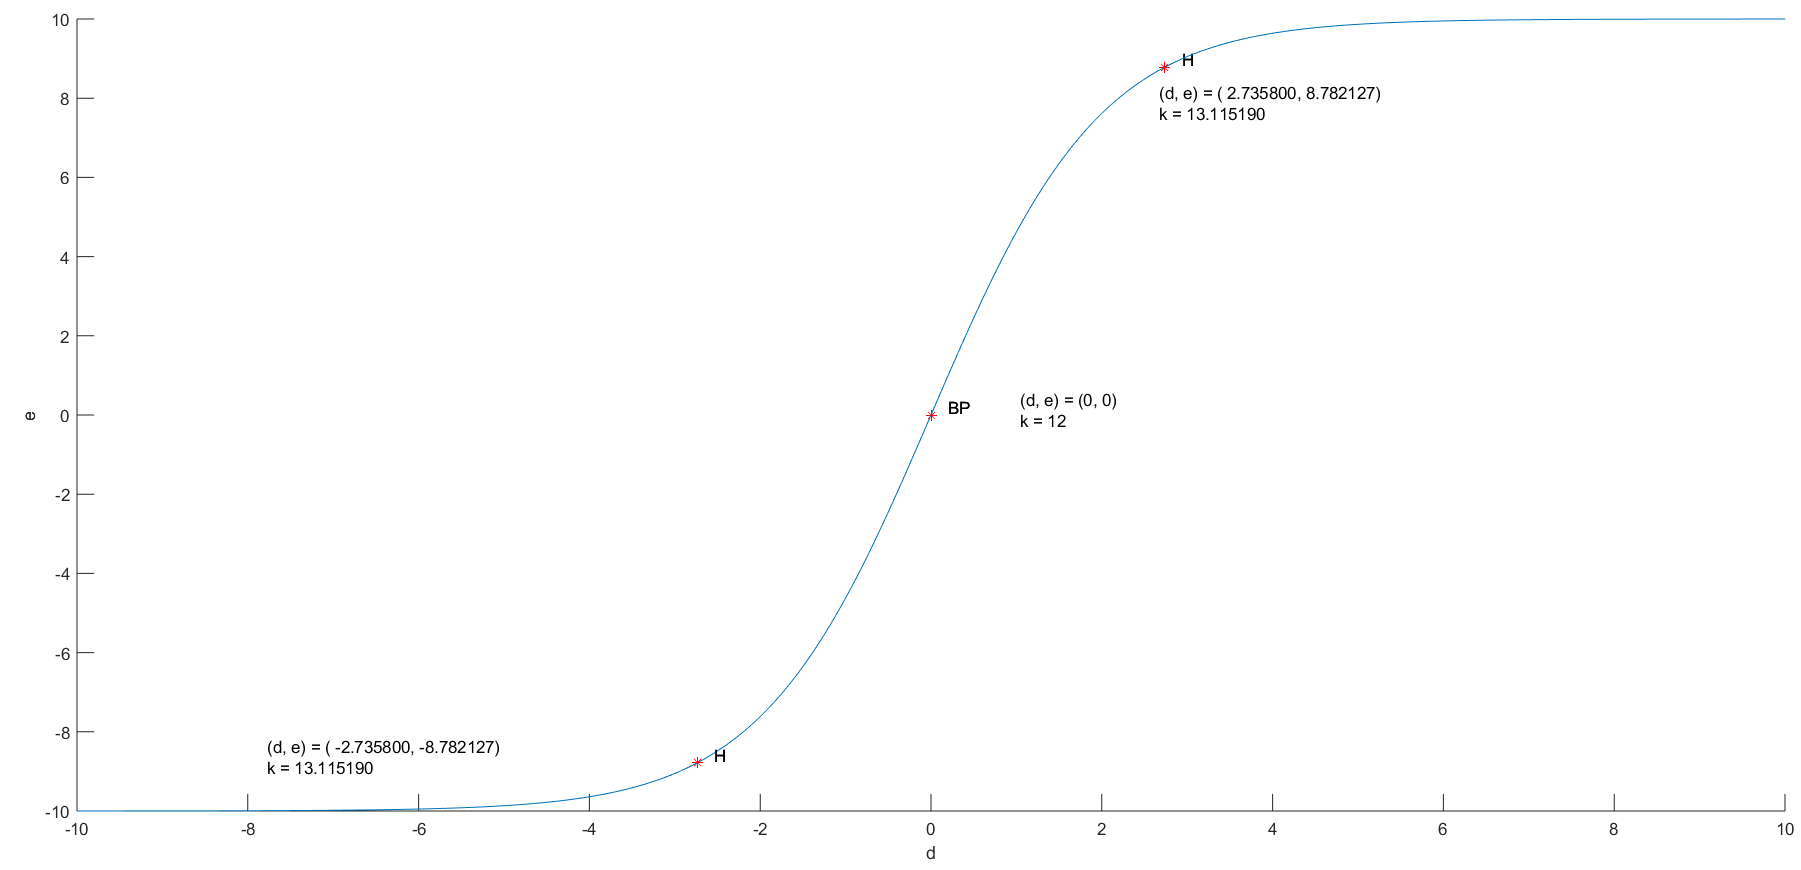
\includegraphics[width=\textwidth]{text/analysis/fig/2by2adapt/bif_hopf.png}}
        \caption{\label{fig:bif_hopf_matcont} Bifurcation diagram for the system in \eqref{eq:diff_dynamics} for  for $g_a=10,\ \tau_a=2$. A saddle node bifurcation occurs at $\alpha = g_a + 2 = 12$ in the origin and Hopf bifurcations at the two off-origin equilibria for $\alpha=13.11590$.}
\end{figure}


\iftrue
   \begin{figure*}[!h]
        \centering
        \begin{subfigure}[b]{1\textwidth}
            \centering
            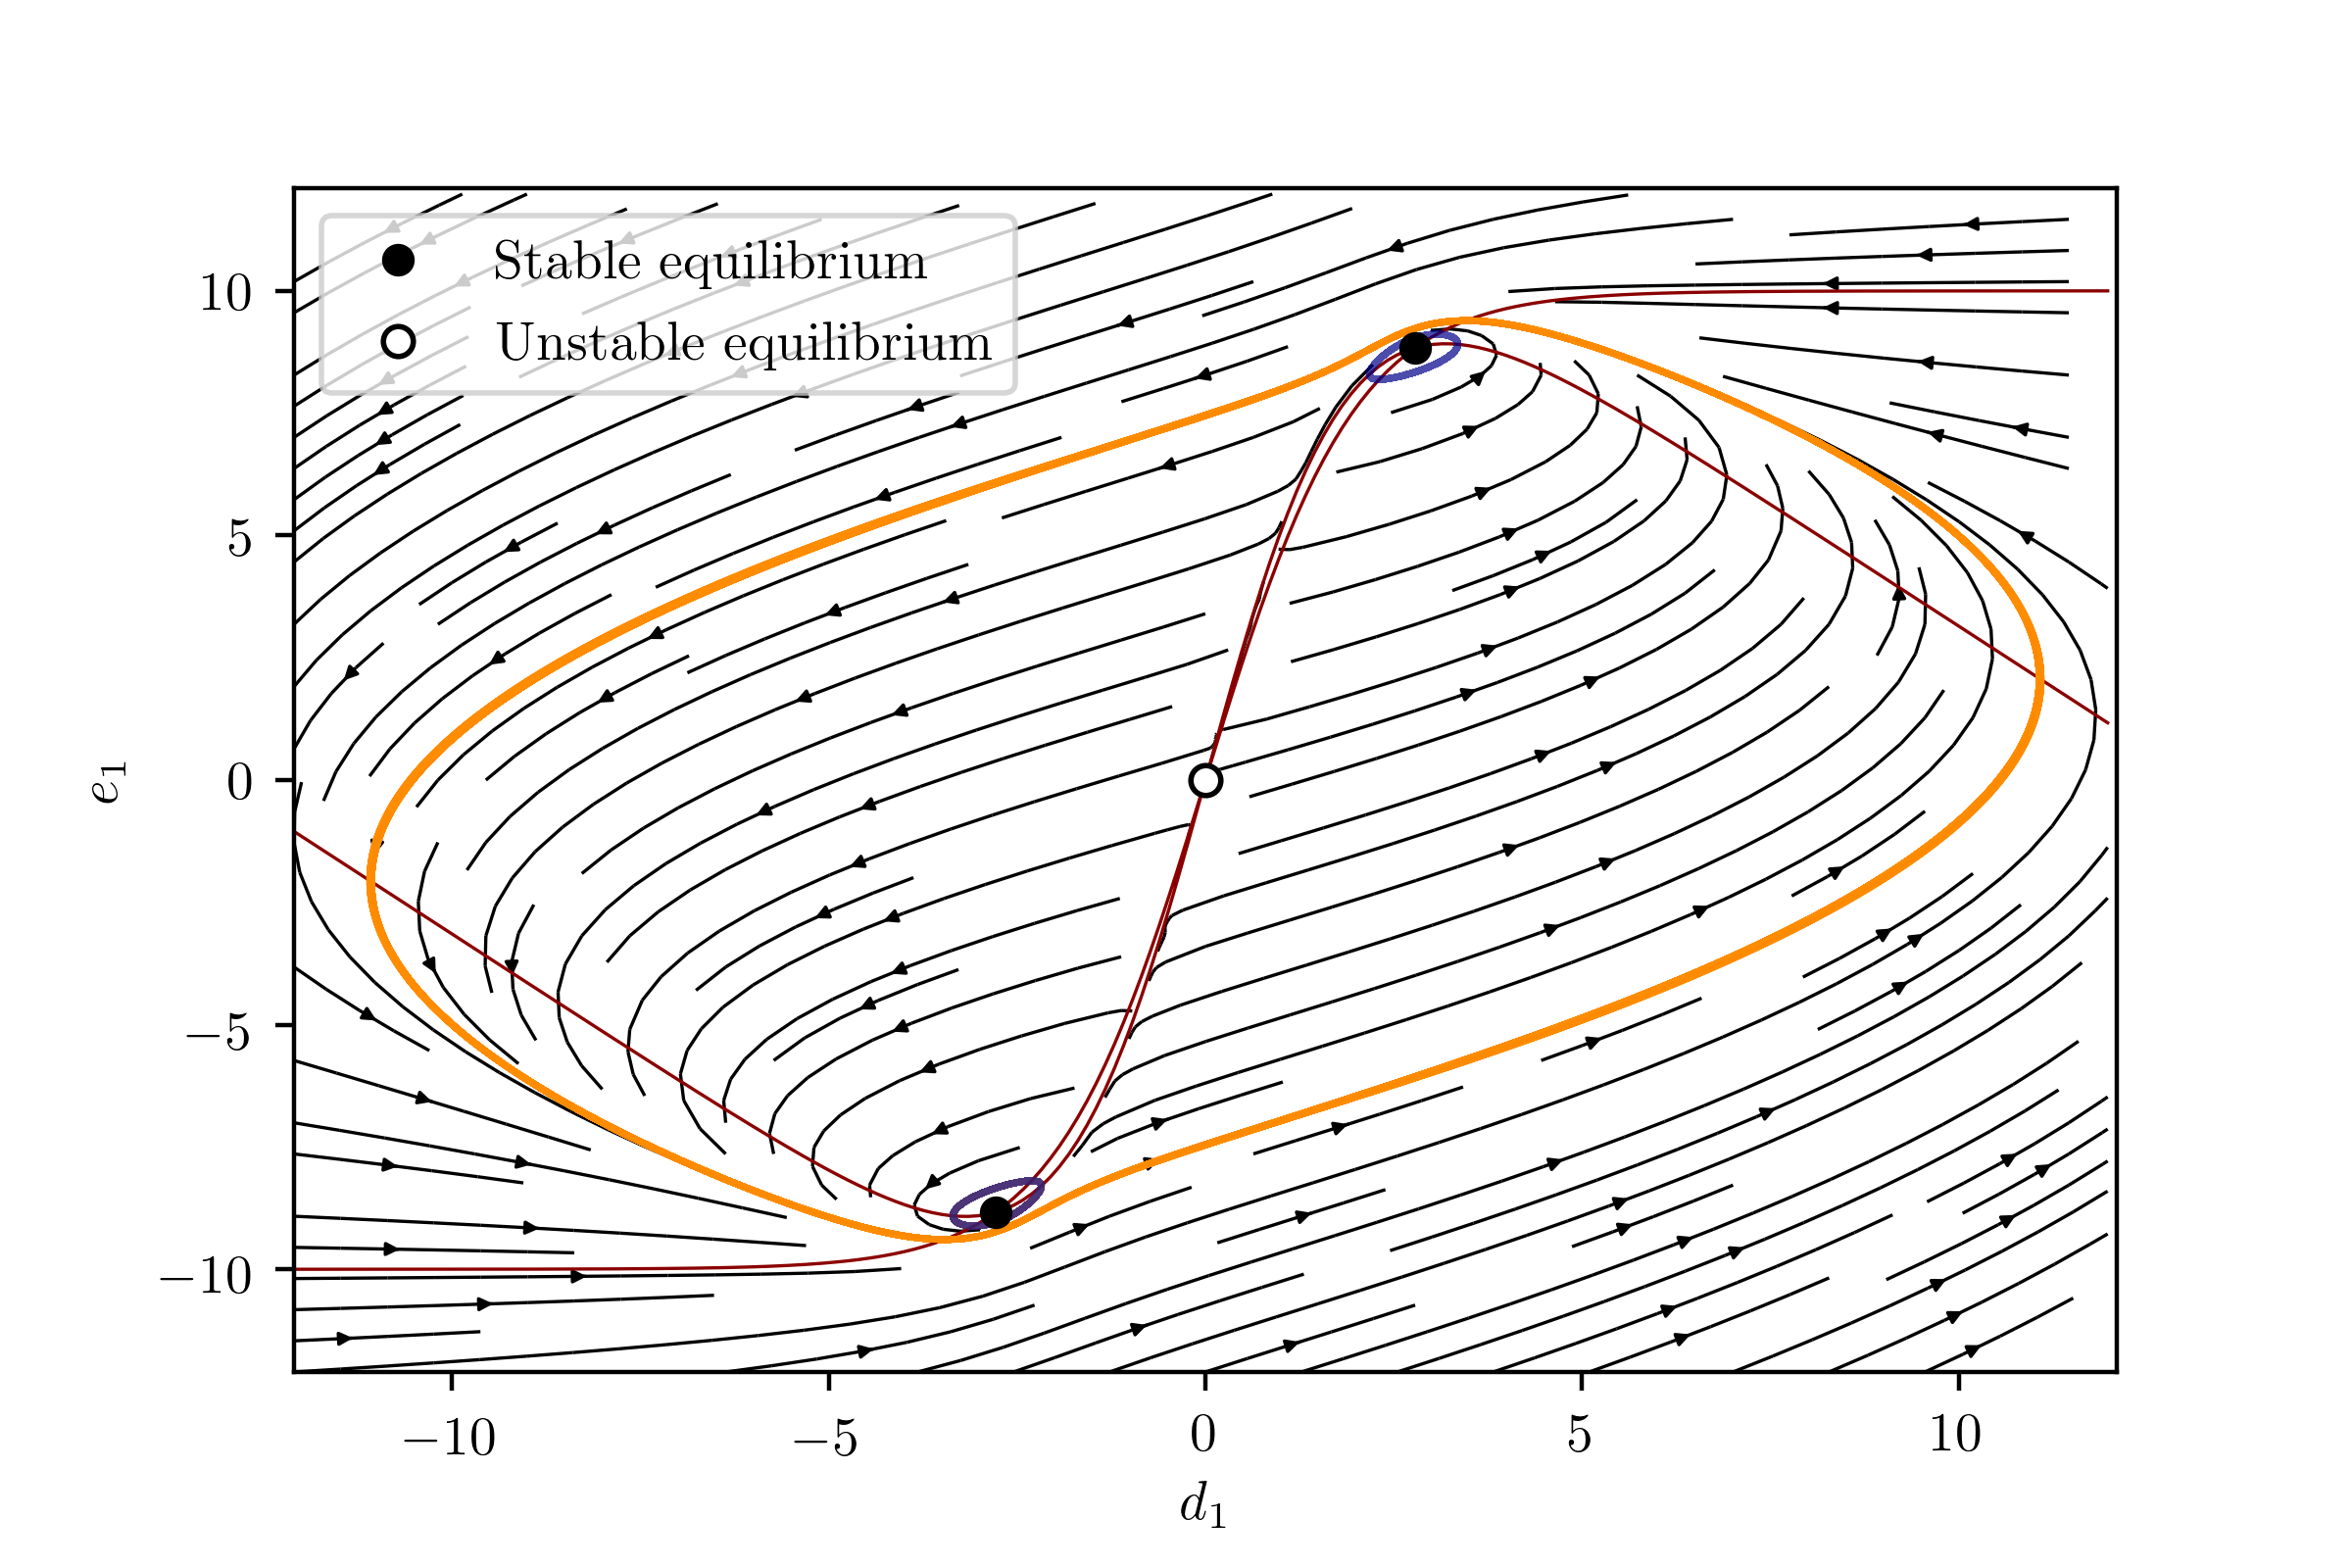
\includegraphics[width=\textwidth]{text/analysis/fig/2by2adapt/streamline_triple_limit.png}
        \end{subfigure}
        \vskip\baselineskip
        \begin{subfigure}[b]{1\textwidth}  
            \centering 
            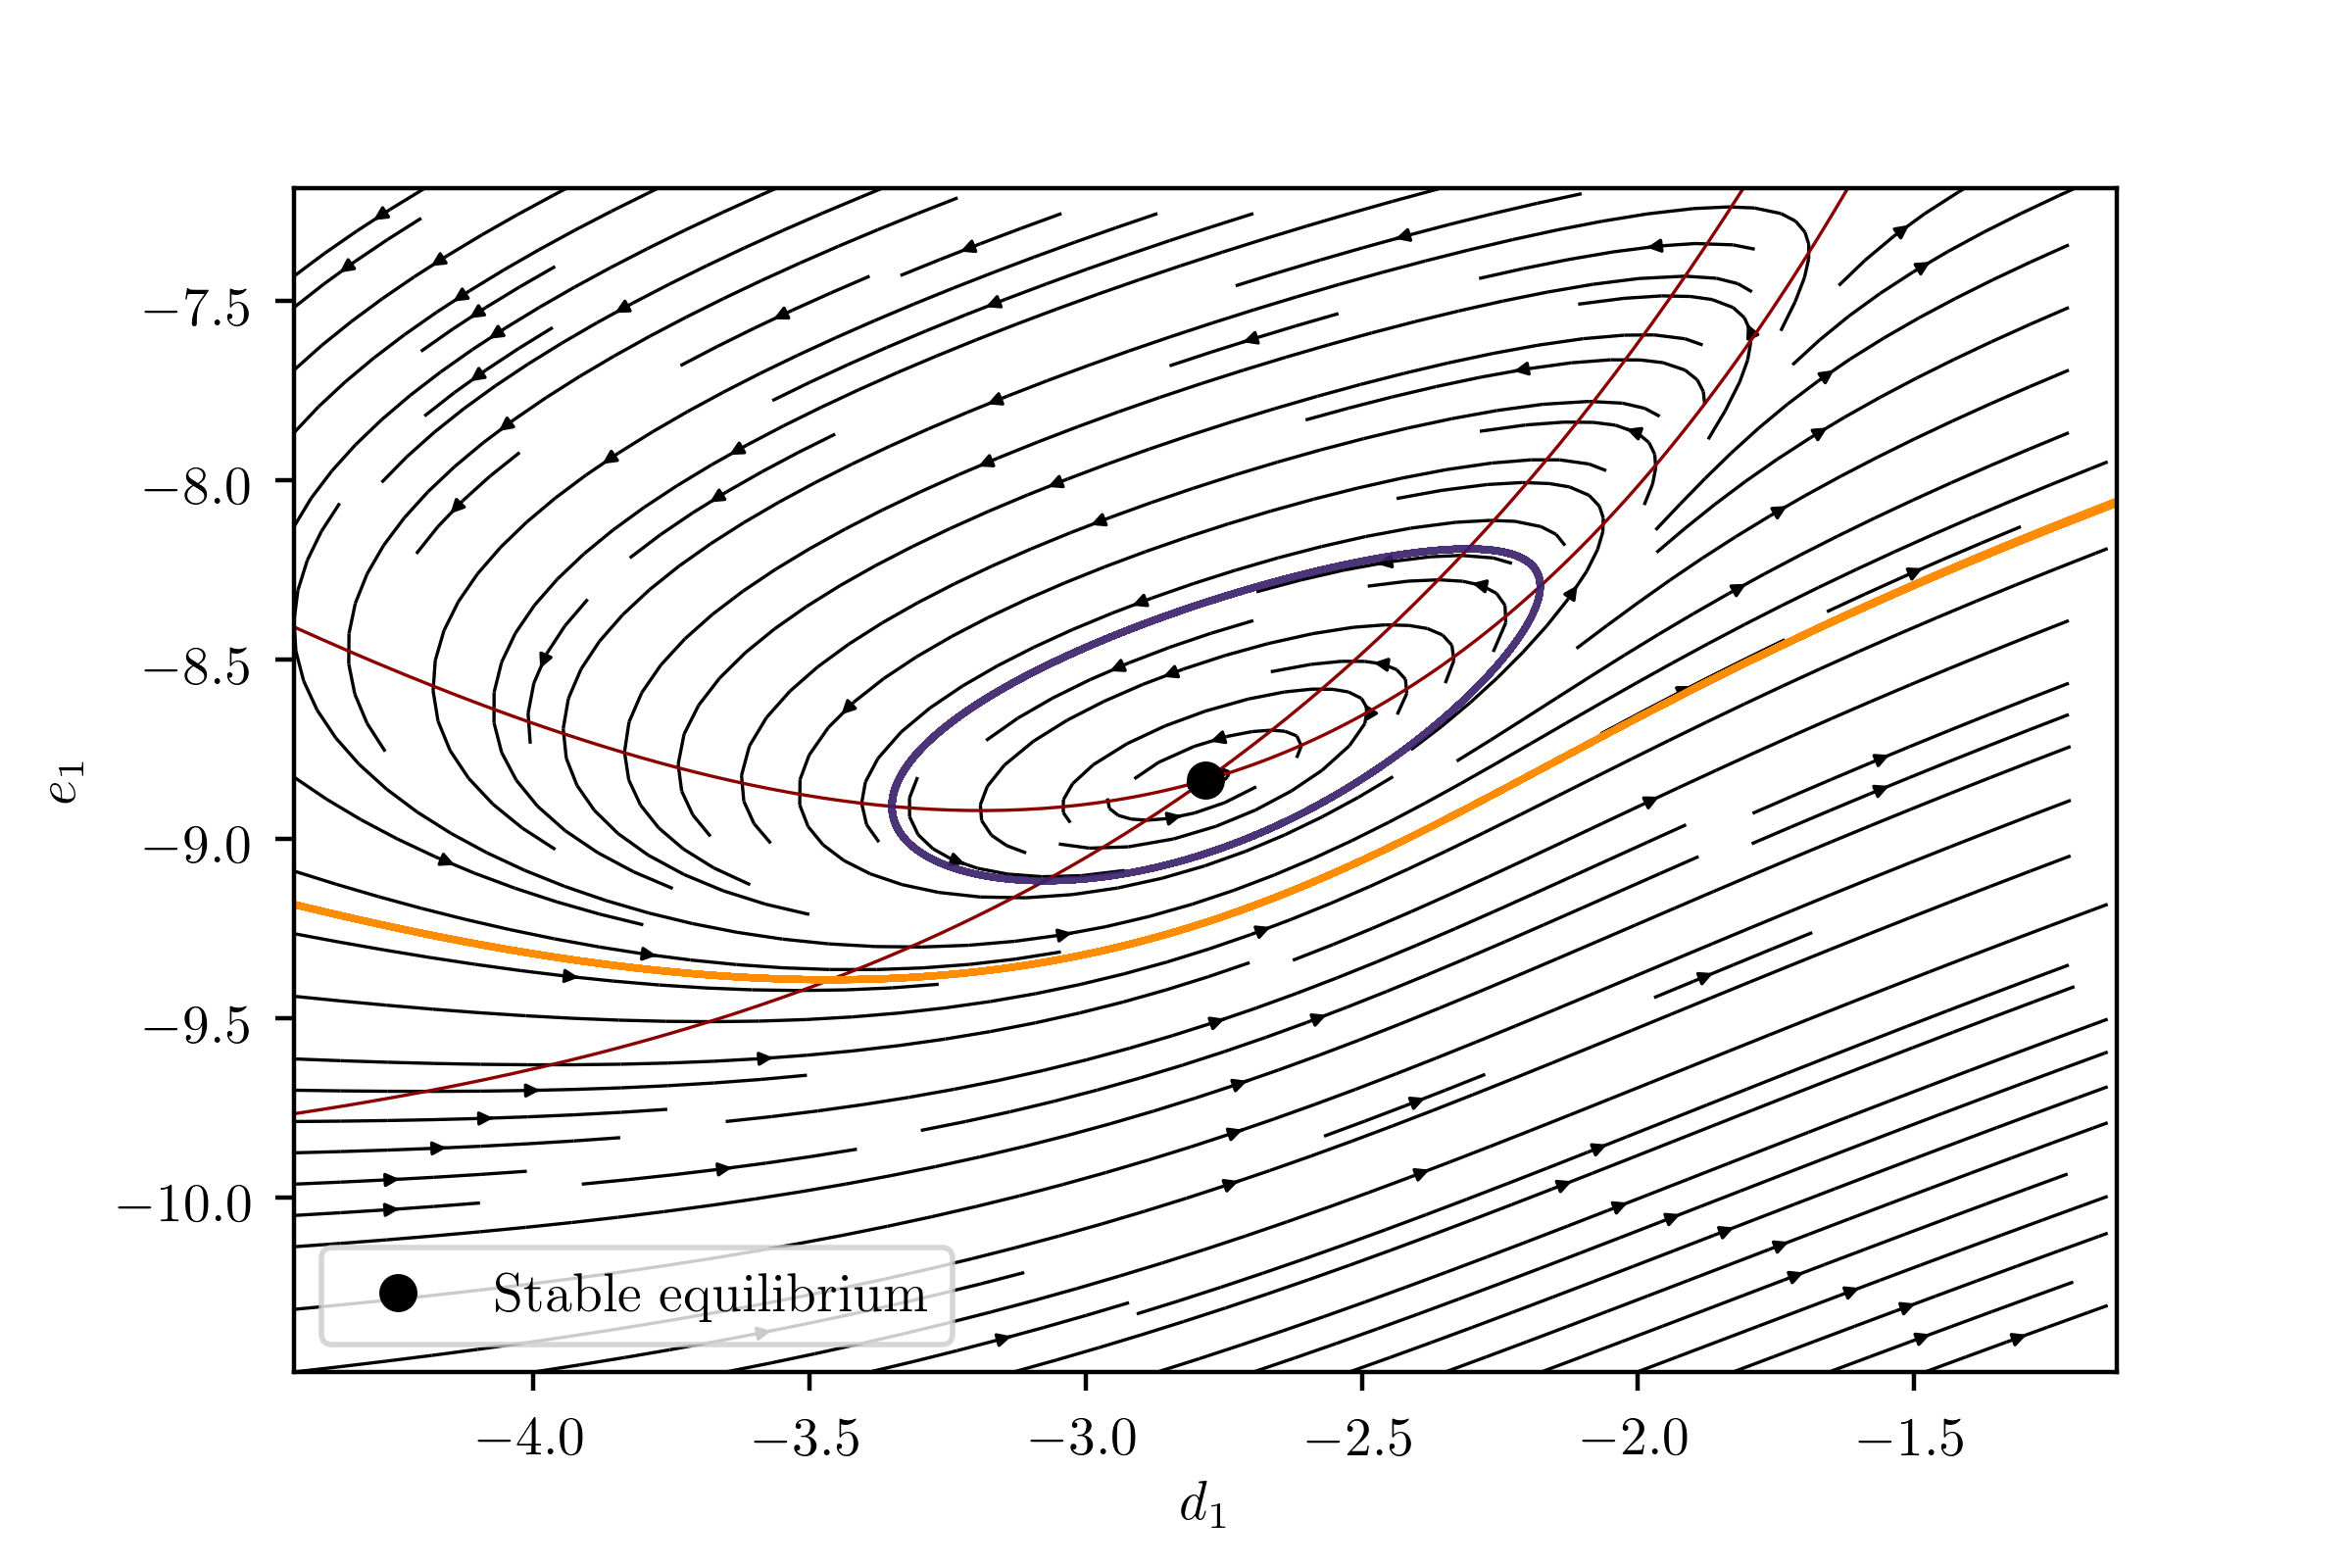
\includegraphics[width=\textwidth]{text/analysis/fig/2by2adapt/streamline_fixed_zoom.png}
        \end{subfigure}
        \caption{Phase portrait of system in \eqref{eq:diff_dynamics} for $\alpha=13.15,\ g_a=10,\ \tau_a=2$. The nullclines are shown in dark red; the streamline plot is shown in black; the outer stable limit cycle is shown in orange; the inner unstable limit cycles (obtained by backward integration in time) are shown in blue. The two pictures show respectively the overall phase portrait (upper) and a zoom on the unstable limit cycle (lower).} 
        \label{fig:adapt_zoom_tri_limt}
    \end{figure*}
\fi


\begin{figure}[!h]
        \center{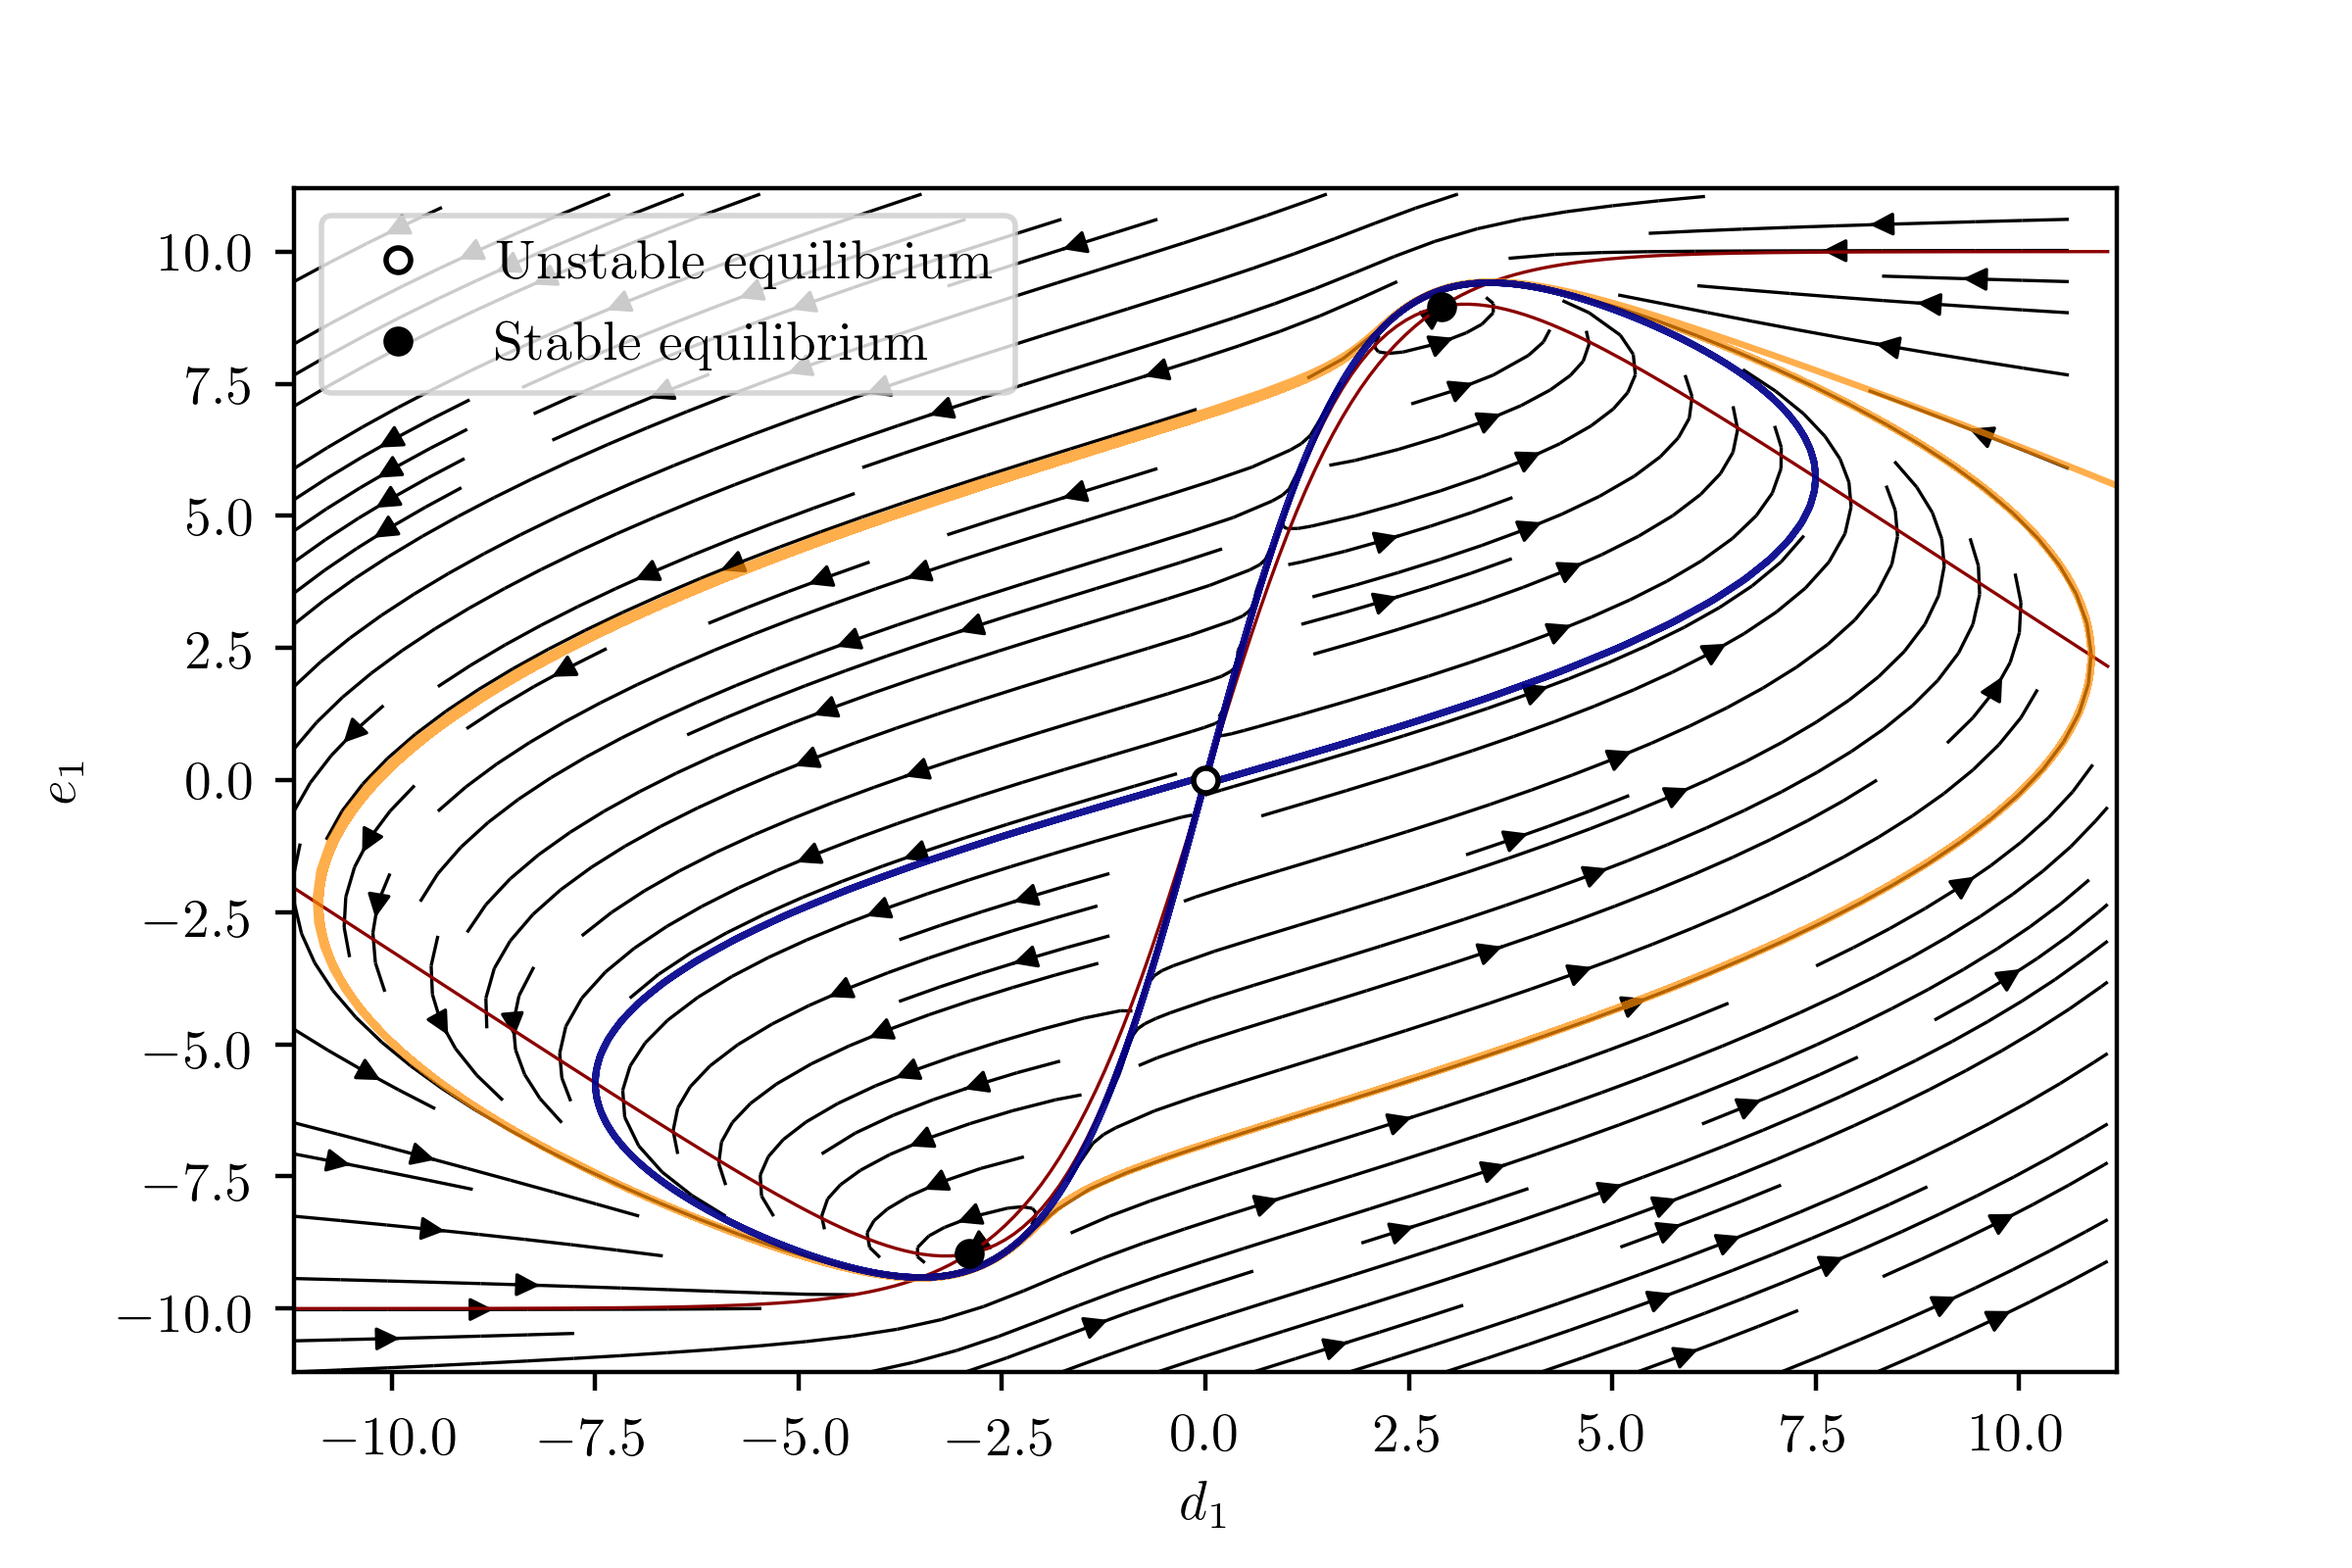
\includegraphics[width=\textwidth]{text/analysis/fig/2by2adapt/streamline_homoclinic.png}}
        \caption{\label{fig:eq2D_cycle_homoclinic} Phase portrait of system in \eqref{eq:diff_dynamics} for $\alpha=13.2422,\ g_a=10,\ \tau_a=2$. The nullclines are shown in dark red; the streamline plot is shown in black; the outer stable limit cycle is shown in orange; the inner unstable limit cycles (obtained by backward integration in time) are shown in blue.}
\end{figure}

\begin{figure}[!h]
        \center{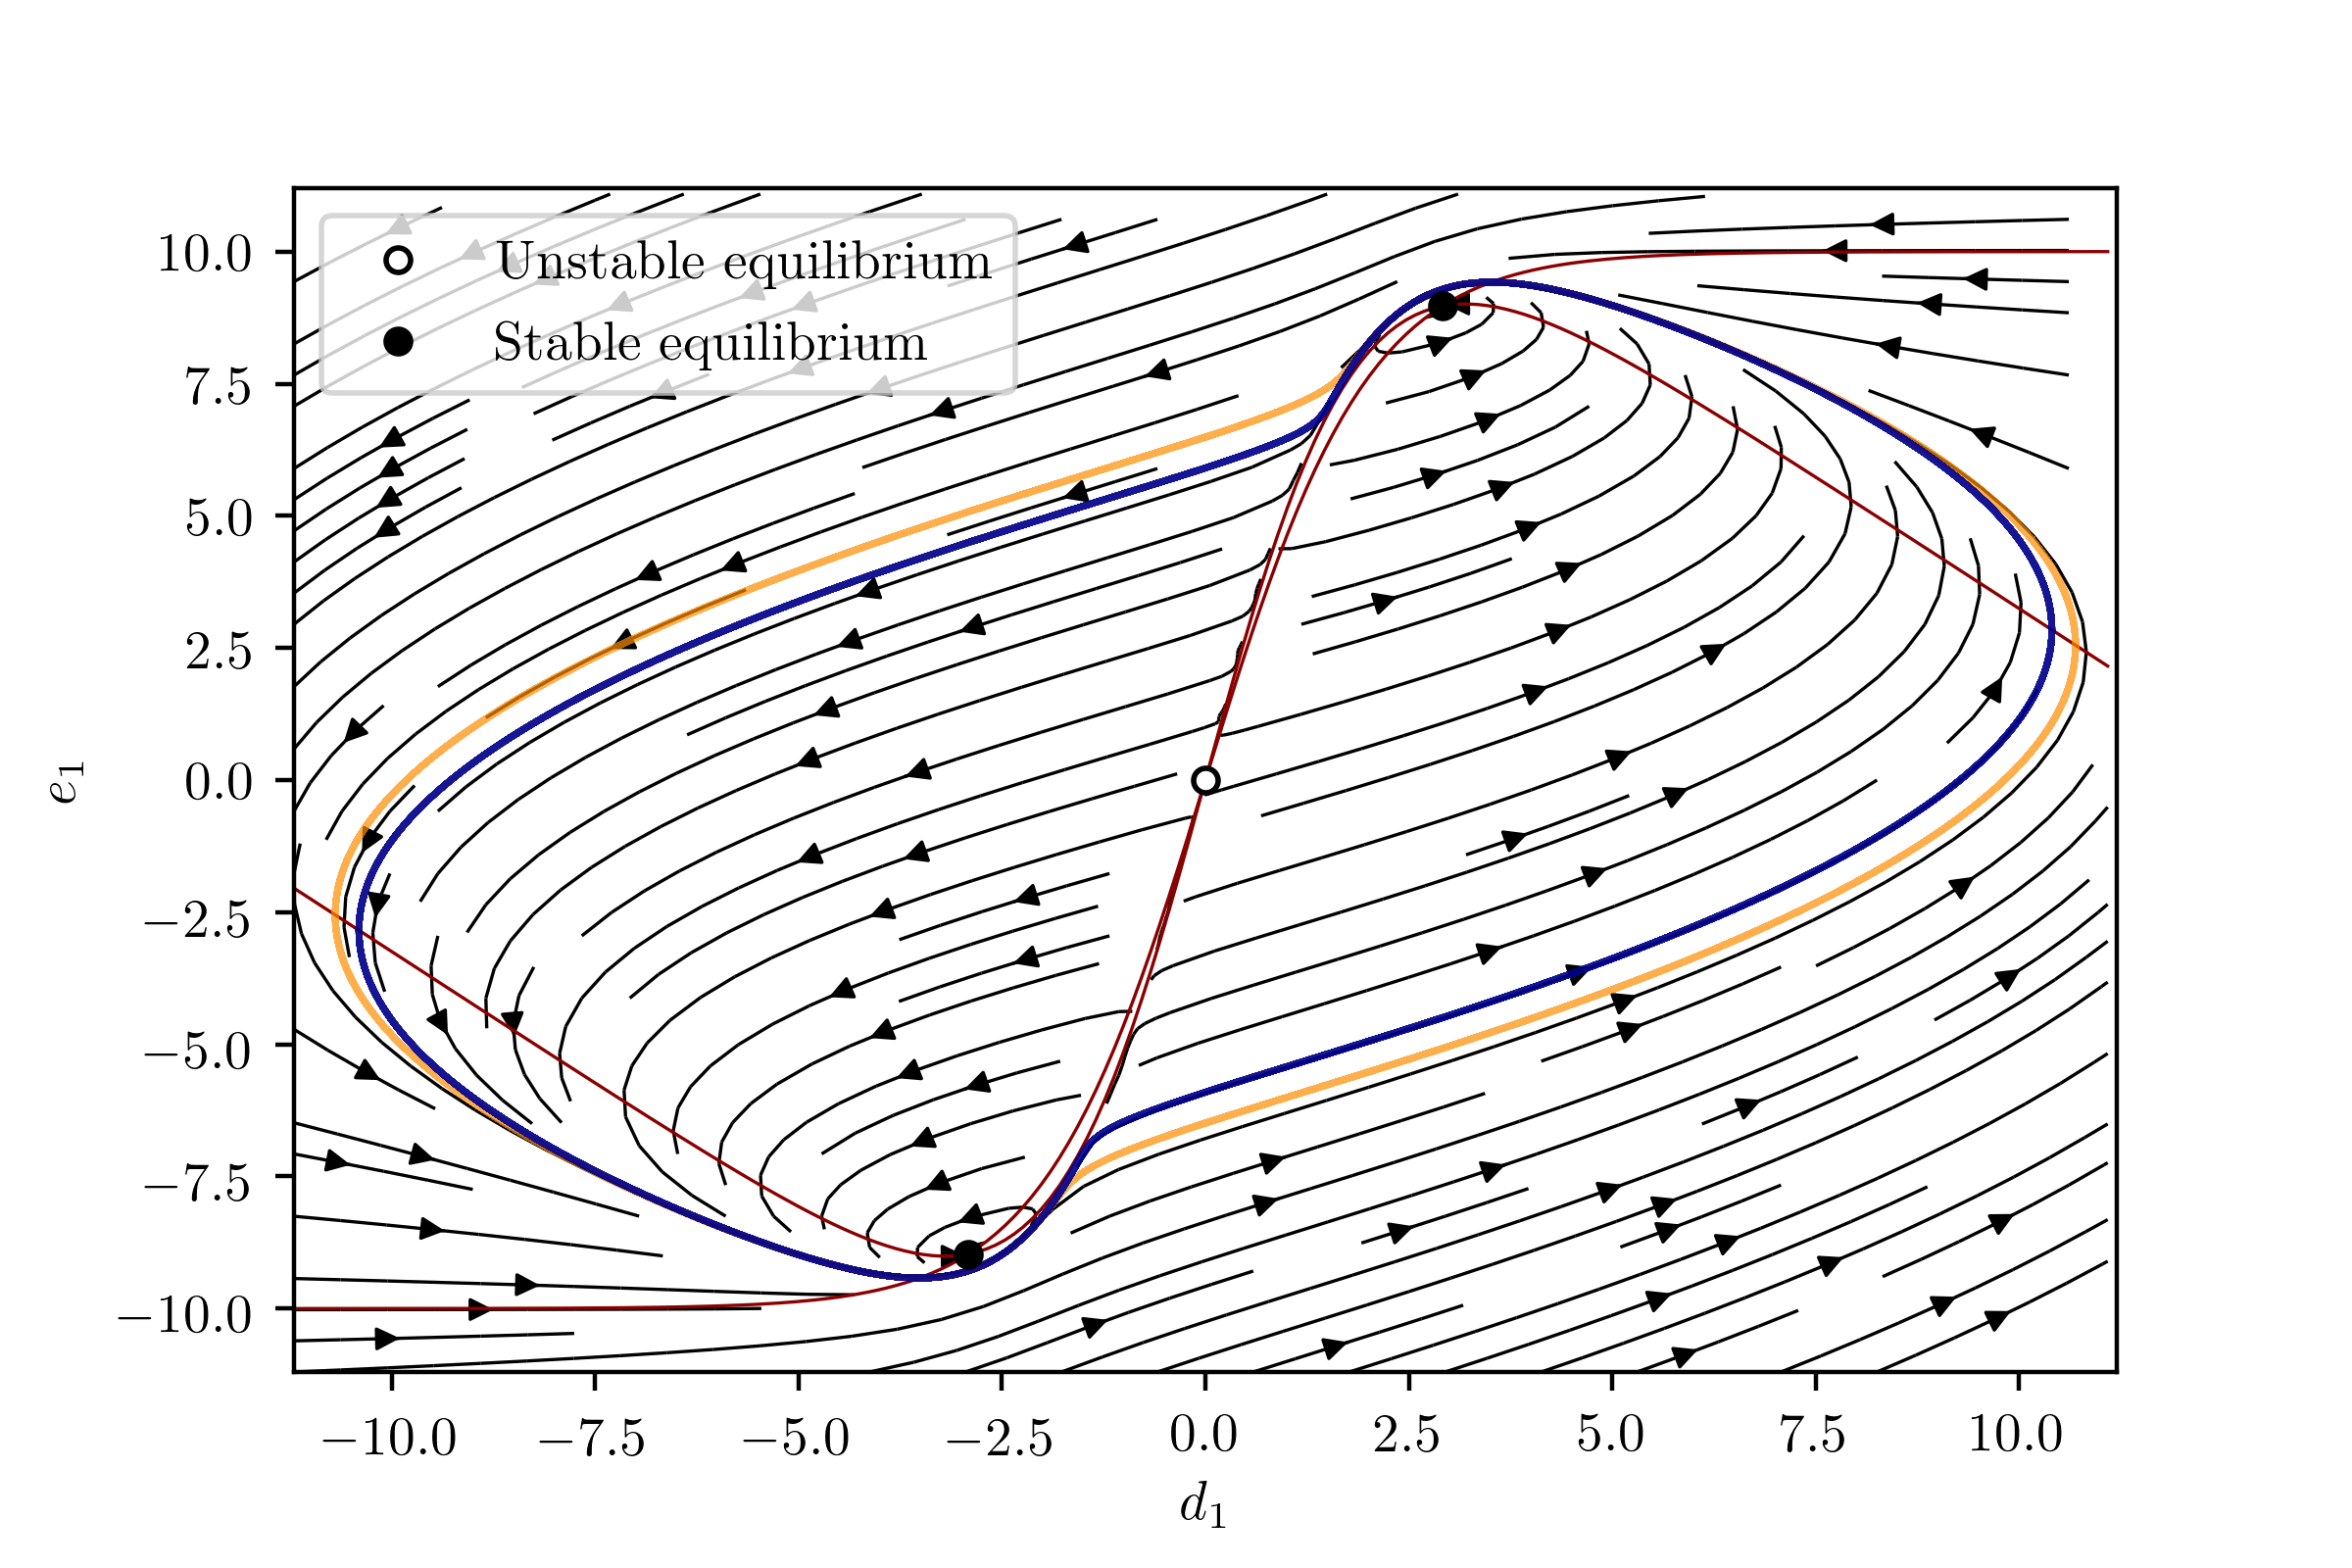
\includegraphics[width=\textwidth]{text/analysis/fig/2by2adapt/streamline_before_collapse.png}}
        \caption{\label{fig:eq2D_cycle_before_collapse} Phase portrait of system in \eqref{eq:diff_dynamics} for $\alpha=13.24605,\ g_a=10,\ \tau_a=2$. The nullclines are shown in dark red; the streamline plot is shown in black; the outer stable limit cycle is shown in orange; the inner unstable limit cycle (obtained by backward integration in time) is shown in blue.}
\end{figure}


\begin{figure}[!h]
        \center{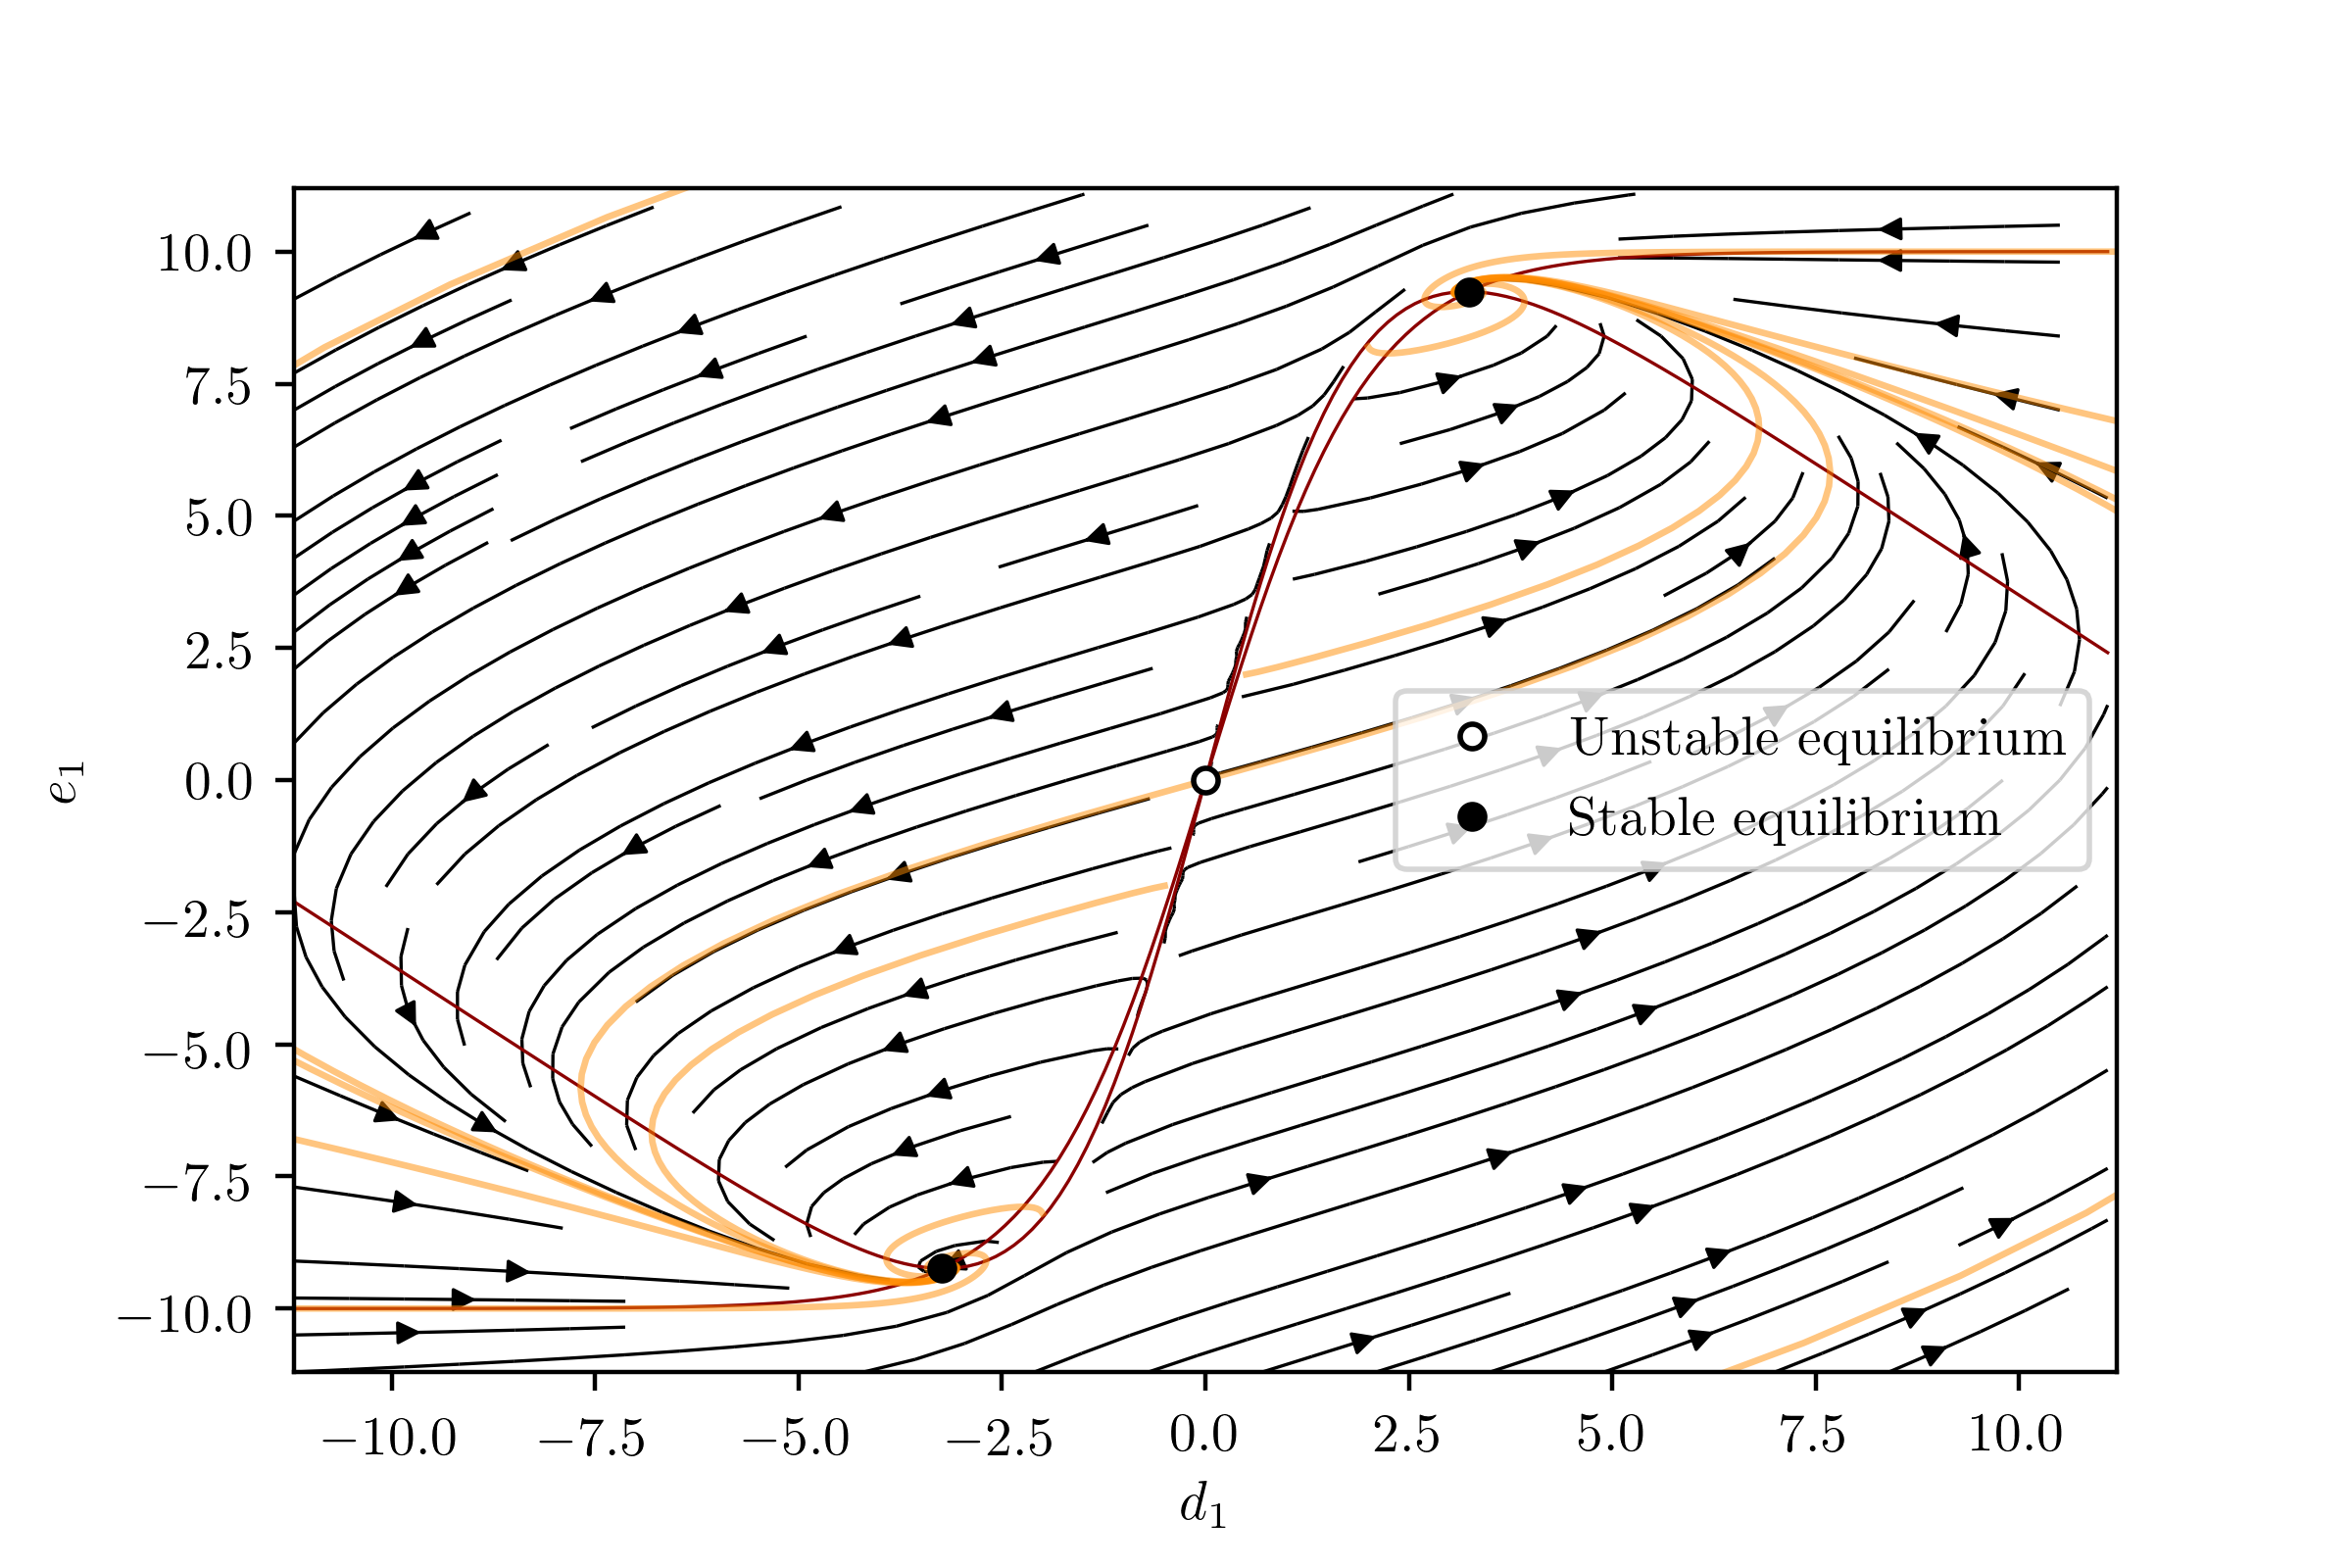
\includegraphics[width=\textwidth]{text/analysis/fig/2by2adapt/streamline_after_collapse.png}}
        \caption{\label{fig:eq2D_cycle_after_collapse} Phase portrait of system in \eqref{eq:diff_dynamics} for $\alpha=13.5,\ g_a=10,\ \tau_a=2$. The nullclines are shown in dark red; the streamline plot is shown in black; several trajectories of the system with different initial conditions are shown in orange. }
\end{figure}

\paragraph{Bifurcation results discussion}
Even for a simple 4-dimensional oscillator, the dynamics of the system is quite rich and it qualitatively varies according to the variation of the parameter $\alpha$. In order to verify the bifurcation analysis performed on the \cref{eq:diff_dynamics} we simulate the original system in \cref{eq:complete_dynamics}.
We chose as an explanatory example the system with $\tau=2,\ g_a=10$. The system's behaviour above can be resumed as follows:
\begin{itemize}
    \item One globally stable equilibrium point with $\alpha<2(1+\frac{1}{\tau_a})=3$ (\cref{fig:eq2D_focus})
    \item One globally stable limit cycle with $2(1+\frac{1}{\tau_a}) < \alpha <\alpha^{oo}$, $ g_a + 2 < \alpha^{oo} \approx 13.11$. (\cref{fig:eq2D_cycle}). 
    \item One stable limit cycle and two stable equilibria with $13.11 \lessapprox \alpha \lessapprox 13.24605$ (\cref{fig:adapt_zoom_tri_limt}). 
    \item Two stable equilibria with $\alpha \gtrapprox 13.24605$ (\cref{fig:eq2D_cycle_after_collapse})
\end{itemize}
